% BEGIN SETUP

% ============================ new frame ==========================================>
% END
% BEGIN ANALYSIS
\subsection{Analysis}
% ============================ FRAME 19 ==========================================>
\begin{frame}
	\frametitle{Waveforms}
	\vspace*{-20pt}
	\begin{center}
		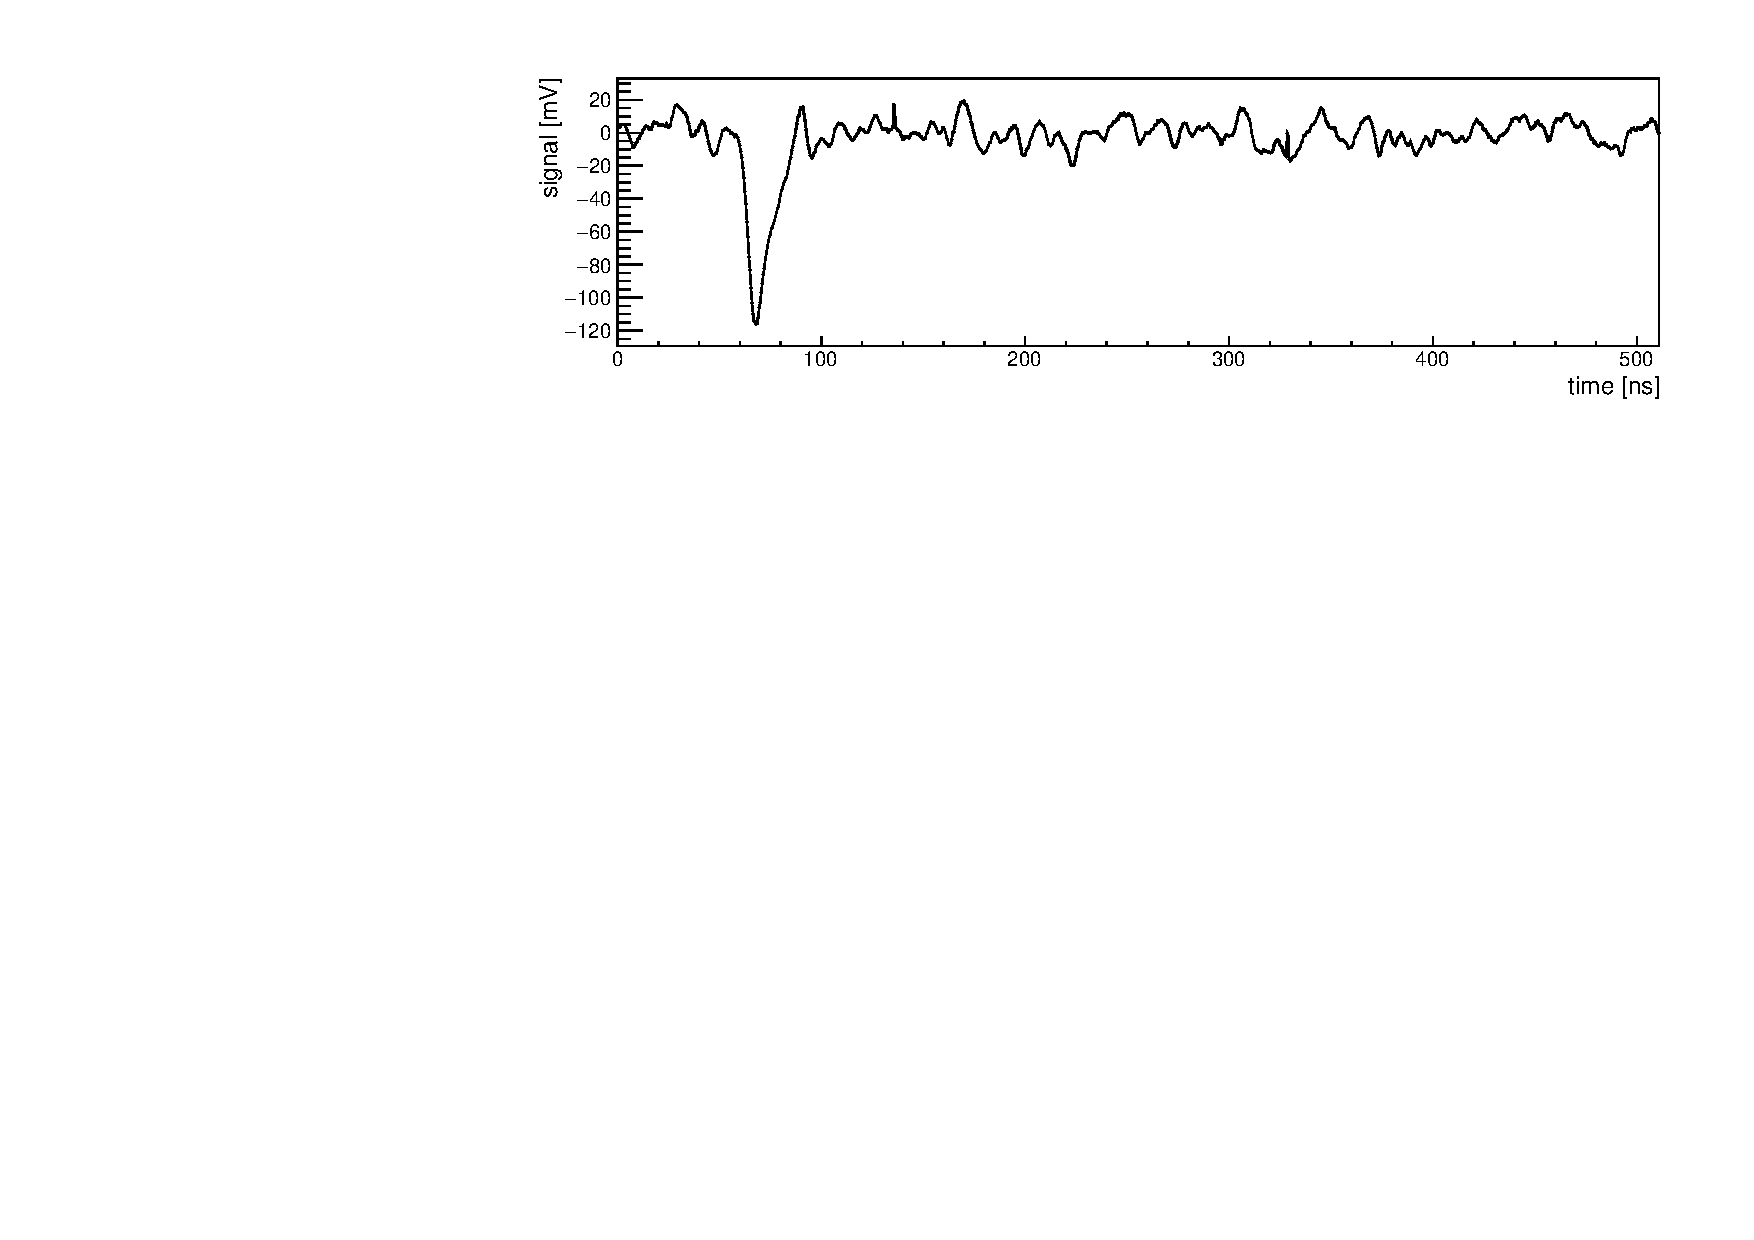
\includegraphics[angle=270, width=.7\textwidth]{SignalWaveform}\\
		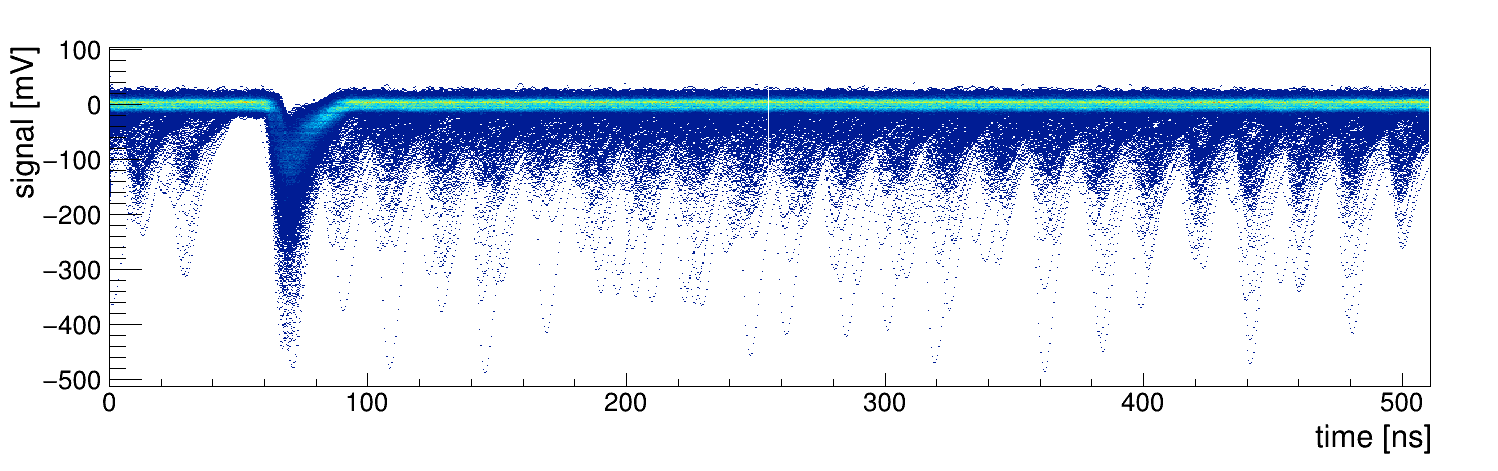
\includegraphics[width=.7\textwidth]{SignalWaveforms5000}
	\end{center}
	\begin{itemize}
		\item most frequented peak (\SI{\sim70}{ns}): triggered signal
		\item other peaks originate from other buckets ($\rightarrow$ resolve beam structure of \SI{\approx19.7}{ns})
		\item system does not allow signals in pre-signal bucket due to fastOR trigger deadtime
	\end{itemize}
\end{frame}
% ============================ FRAME 20 ==========================================>
\begin{frame}
	\frametitle{Pulse Height Calculation}
	\vspace*{-5pt}
	\begin{center}
		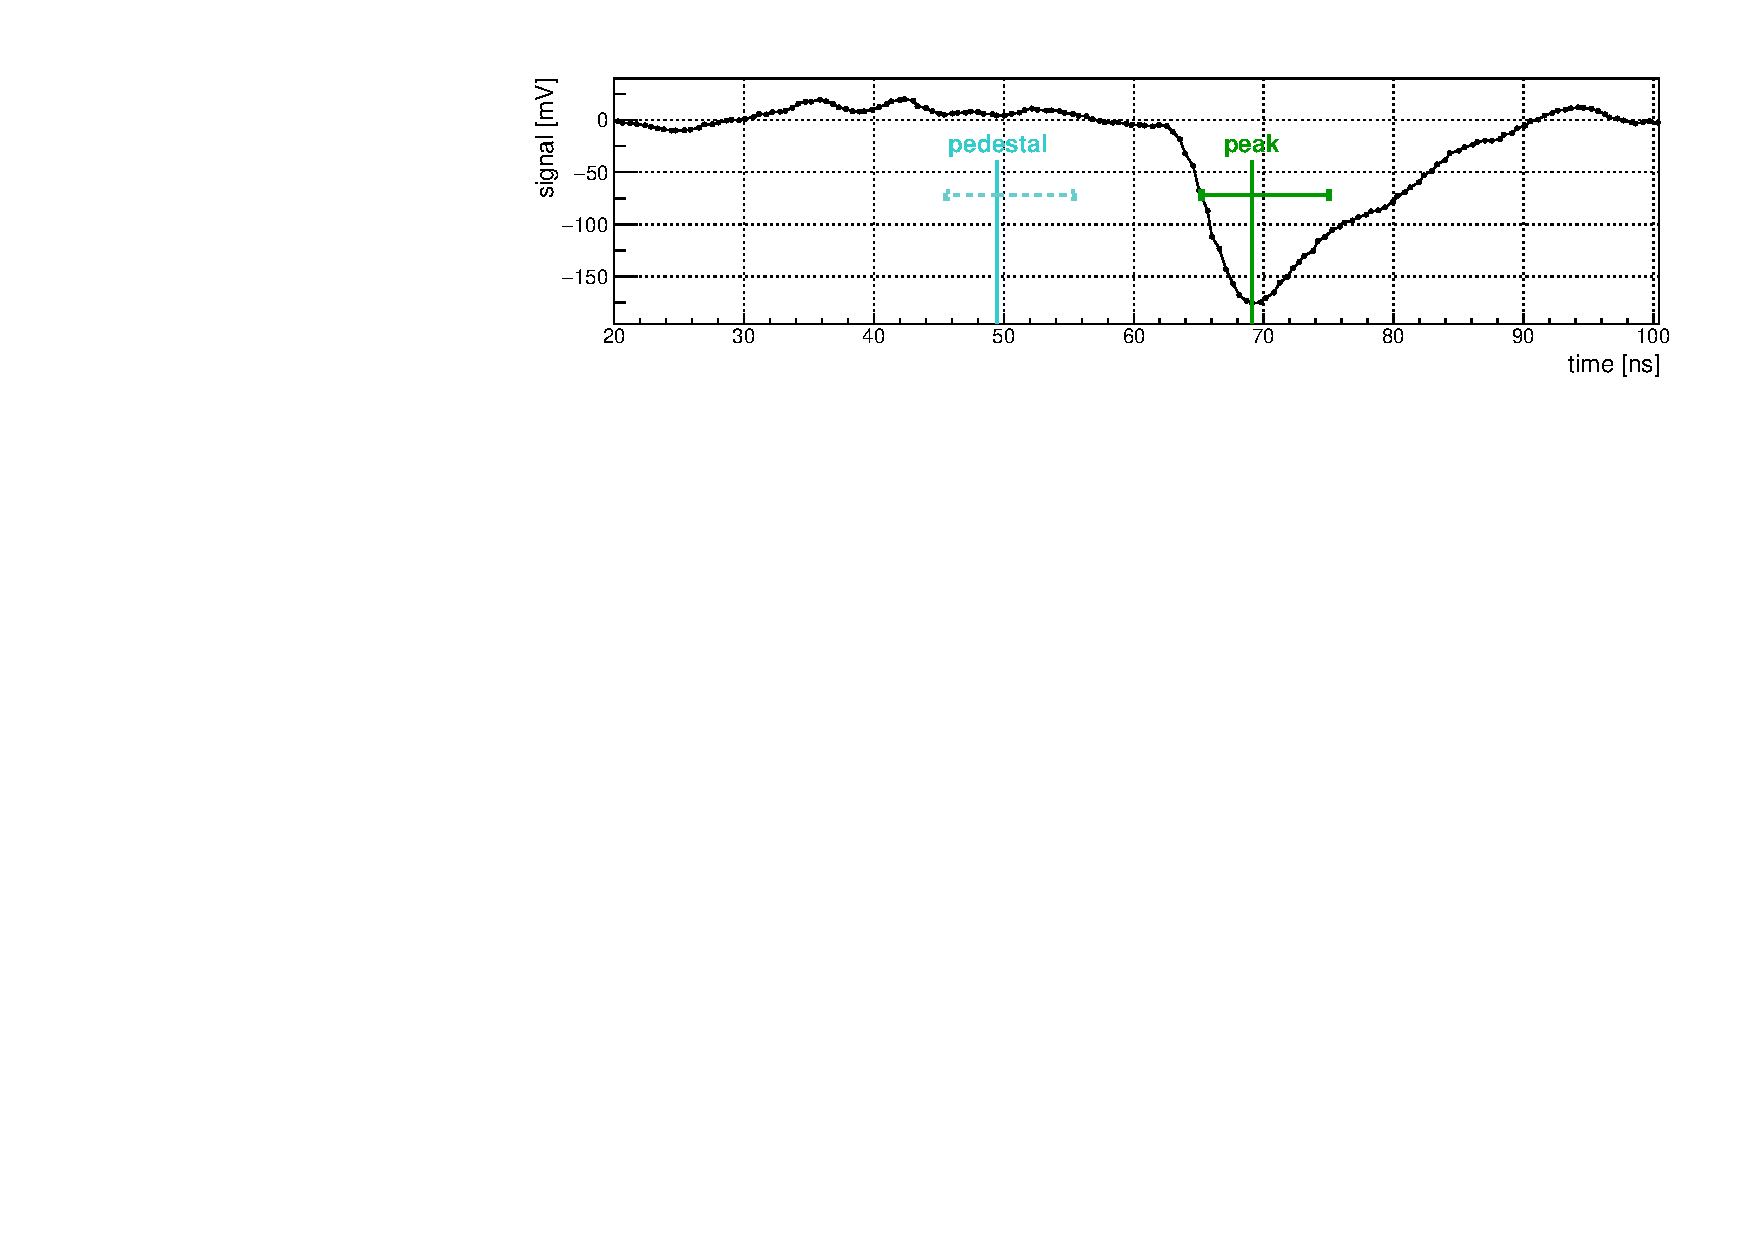
\includegraphics[angle=270, width=.8\textwidth]{intpeaks}\\
	\end{center}
	\vspace*{-5pt}
	\begin{itemize}
		\setlength{\itemsep}{\fill}
		\item finding the peak in the signal region
		\item integrating the signal in time fixed asymmetric integral around peak
		\item time averaging
		\item same procedure for pedestal (base line $\rightarrow$ noise)
		\item optimising the integral width by highest SNR (Integral / Pedestal Sigma)
		\item subtracting the pedestal from the signal integral on event-wise basis 
	\end{itemize}
\end{frame}
% ============================ FRAME 21 ==========================================>
\begin{frame}
	\frametitle{Event based cuts}
	\vspace*{-7pt}
	\begin{figure} 
		\begin{center}
			\begin{subfigure}{0.45\textwidth}  
				\centering 
				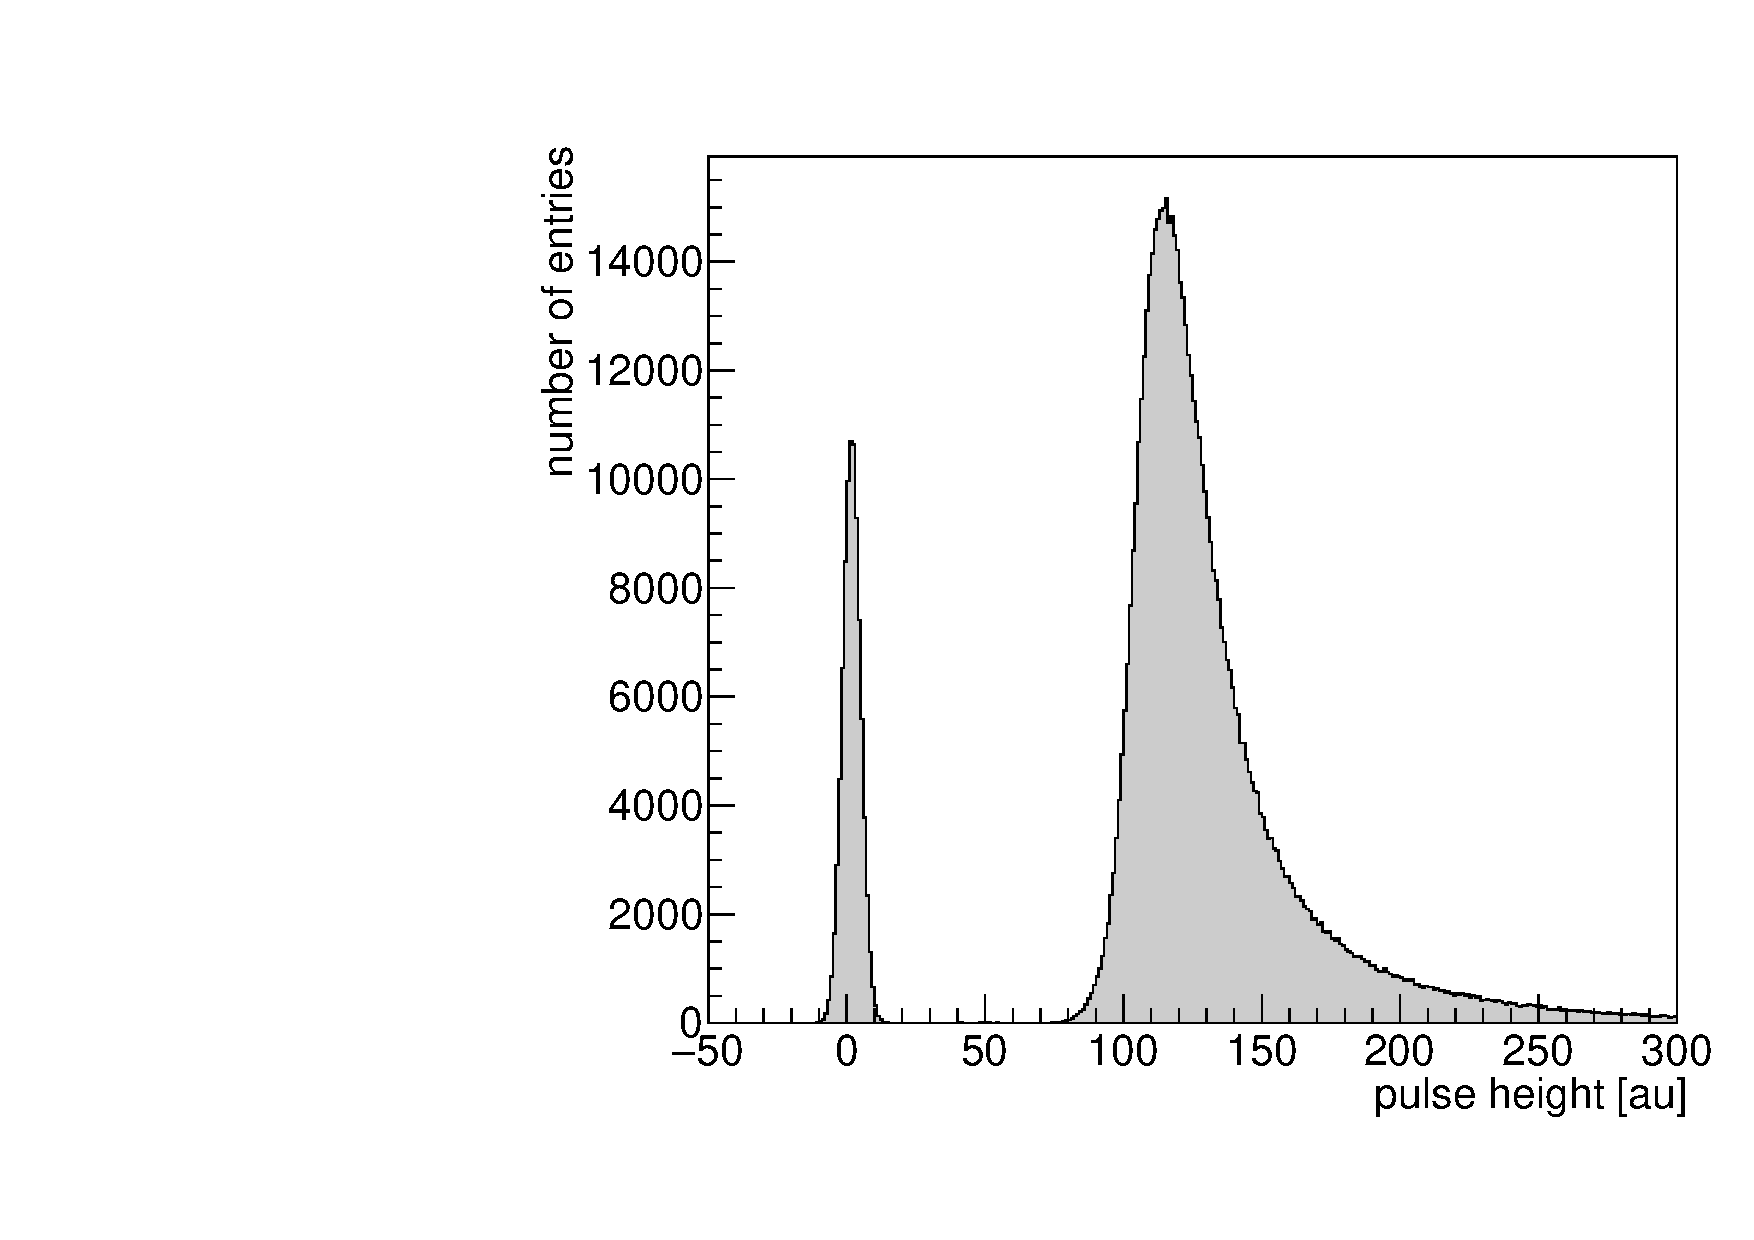
\includegraphics[angle=270, width=.85\textwidth]{DistoNoCuts}
				\caption{no cuts}
			\end{subfigure}
			\ra
			\begin{subfigure}{0.45\textwidth} 
				\centering 
				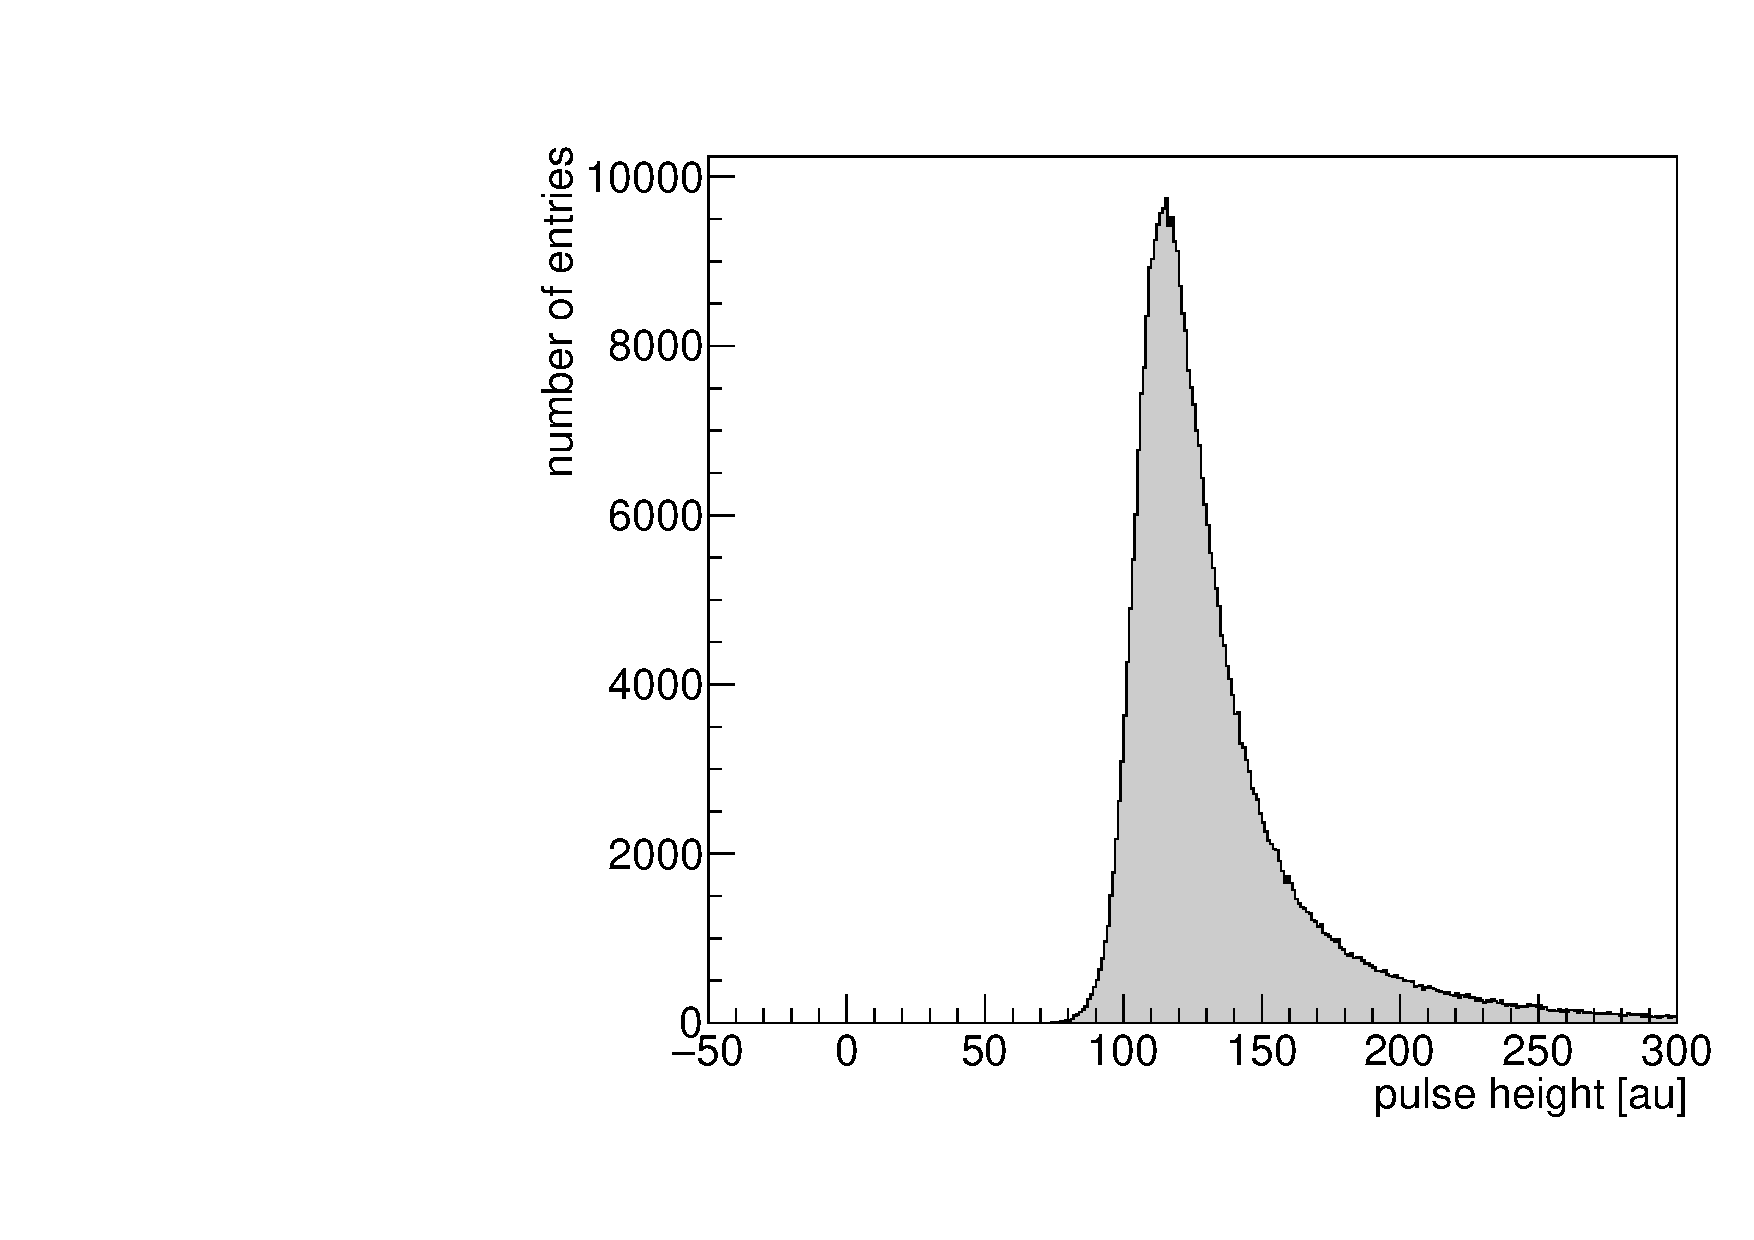
\includegraphics[angle=270, width=.85\textwidth]{DistoCuts}
				\caption{all cuts} 	
			\end{subfigure} 
		\end{center}
	\end{figure}
	\vspace*{-7pt}
	\begin{itemize}
		\setlength{\itemsep}{\fill}
		\item many undesirable events in the full data (no signal, pulser, multiple hits, $\hdots$)
		\item apply cuts to select only signal events (diamond hit by a single pion)
	\end{itemize}
\end{frame}
% ============================ FRAME 22 ==========================================>
\begin{frame}
	\frametitle{Cuts (1)}
	\begin{minipage}{8cm}
		\textbf{\underline{saturated:}}
		\begin{itemize}
			\setlength{\itemsep}{\fill}
			\item saturated waveforms
			\item most likely protons
		\end{itemize}
		\vspace*{1cm}
		\textbf{\underline{pulser:}}
		\begin{itemize}
			\setlength{\itemsep}{\fill}
			\item reference events with different timing
			\item no signal in signal region
		\end{itemize}
		\vspace*{1cm}
		\textbf{\underline{tracks:}}
		\begin{itemize}
			\setlength{\itemsep}{\fill}
			\item only take events with exactly one cluster in each tracking plane
		\end{itemize}
	\end{minipage}
	\begin{minipage}{4cm}
		\vspace*{-5pt}
		\begin{figure}
			\centering
			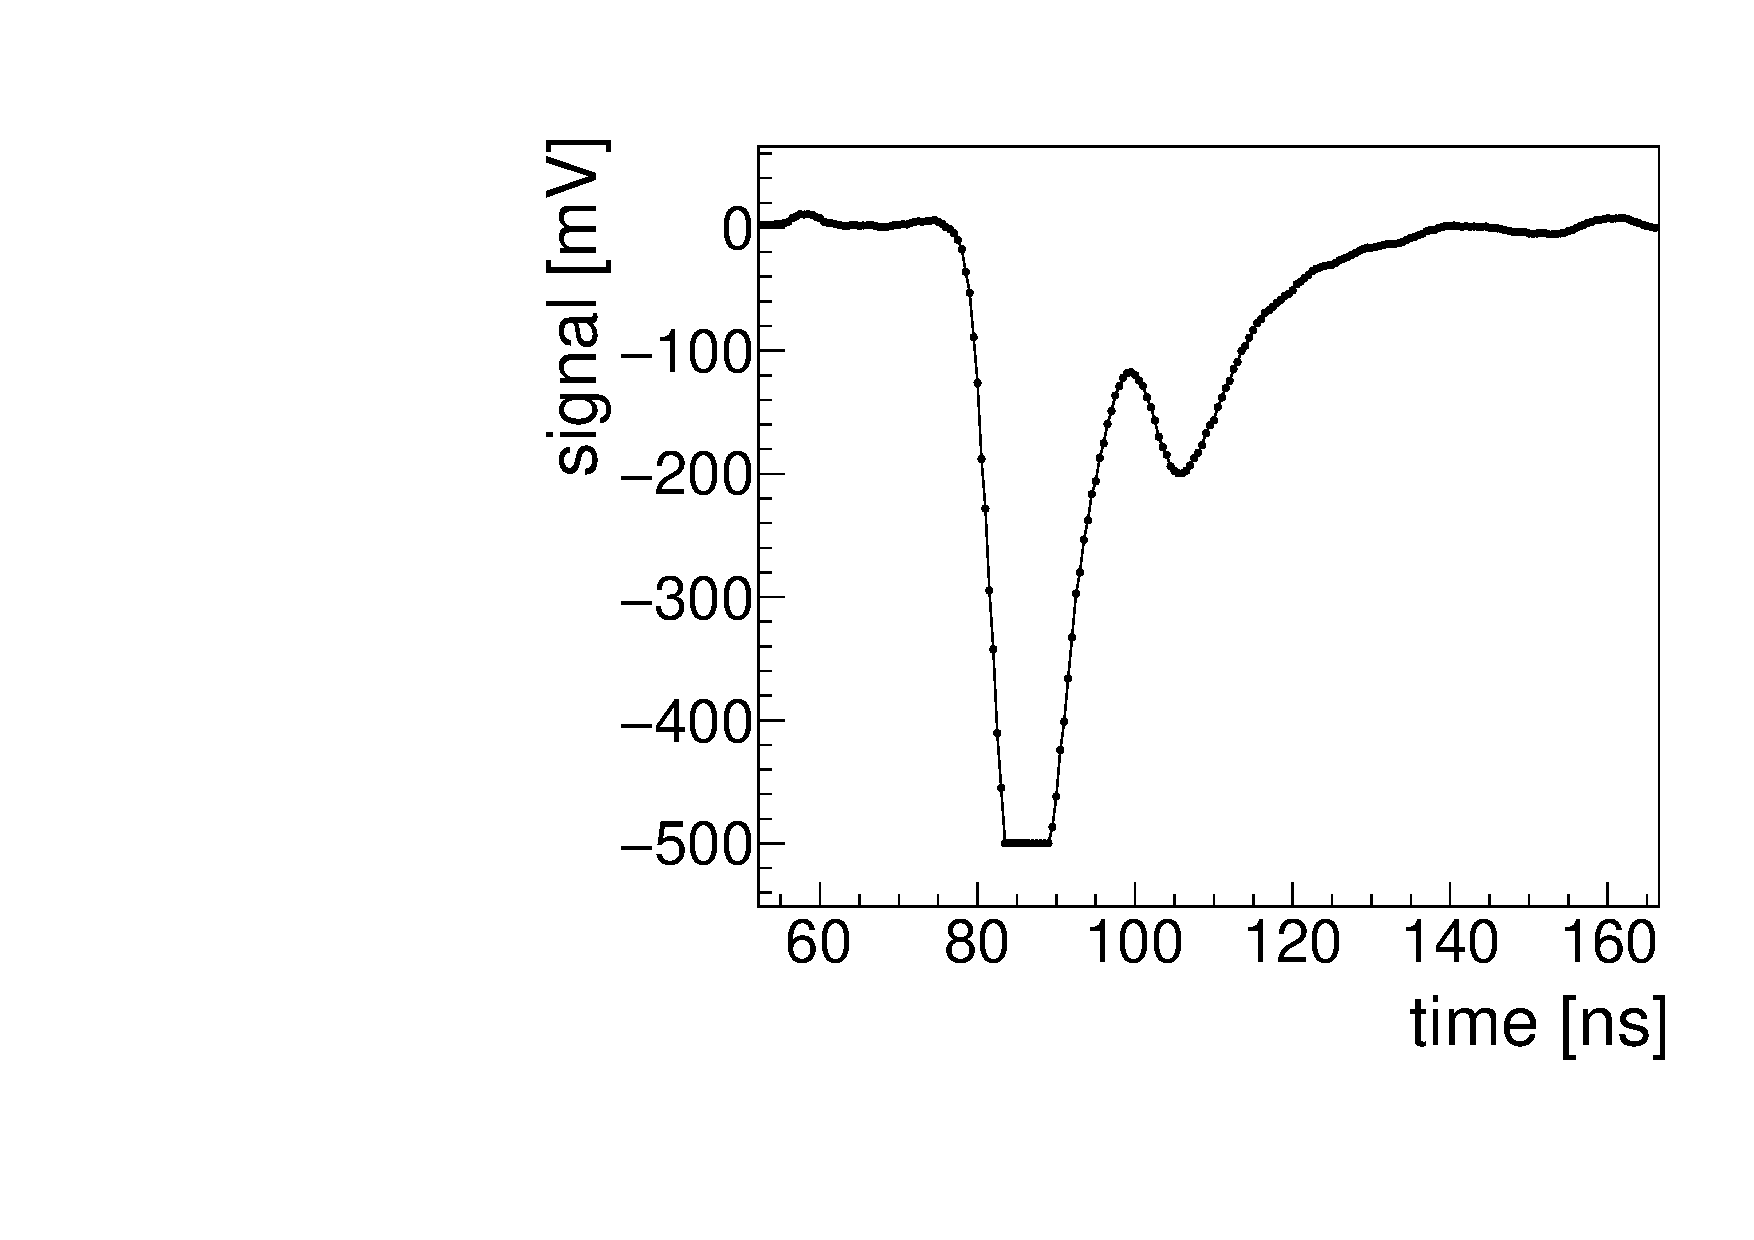
\includegraphics[angle=270, width=3.5cm]{Sat}
			\vspace*{-8pt}
			\caption{saturated waveform}
		\end{figure}
		\vspace*{-25pt}
		\begin{figure}
			\centering
			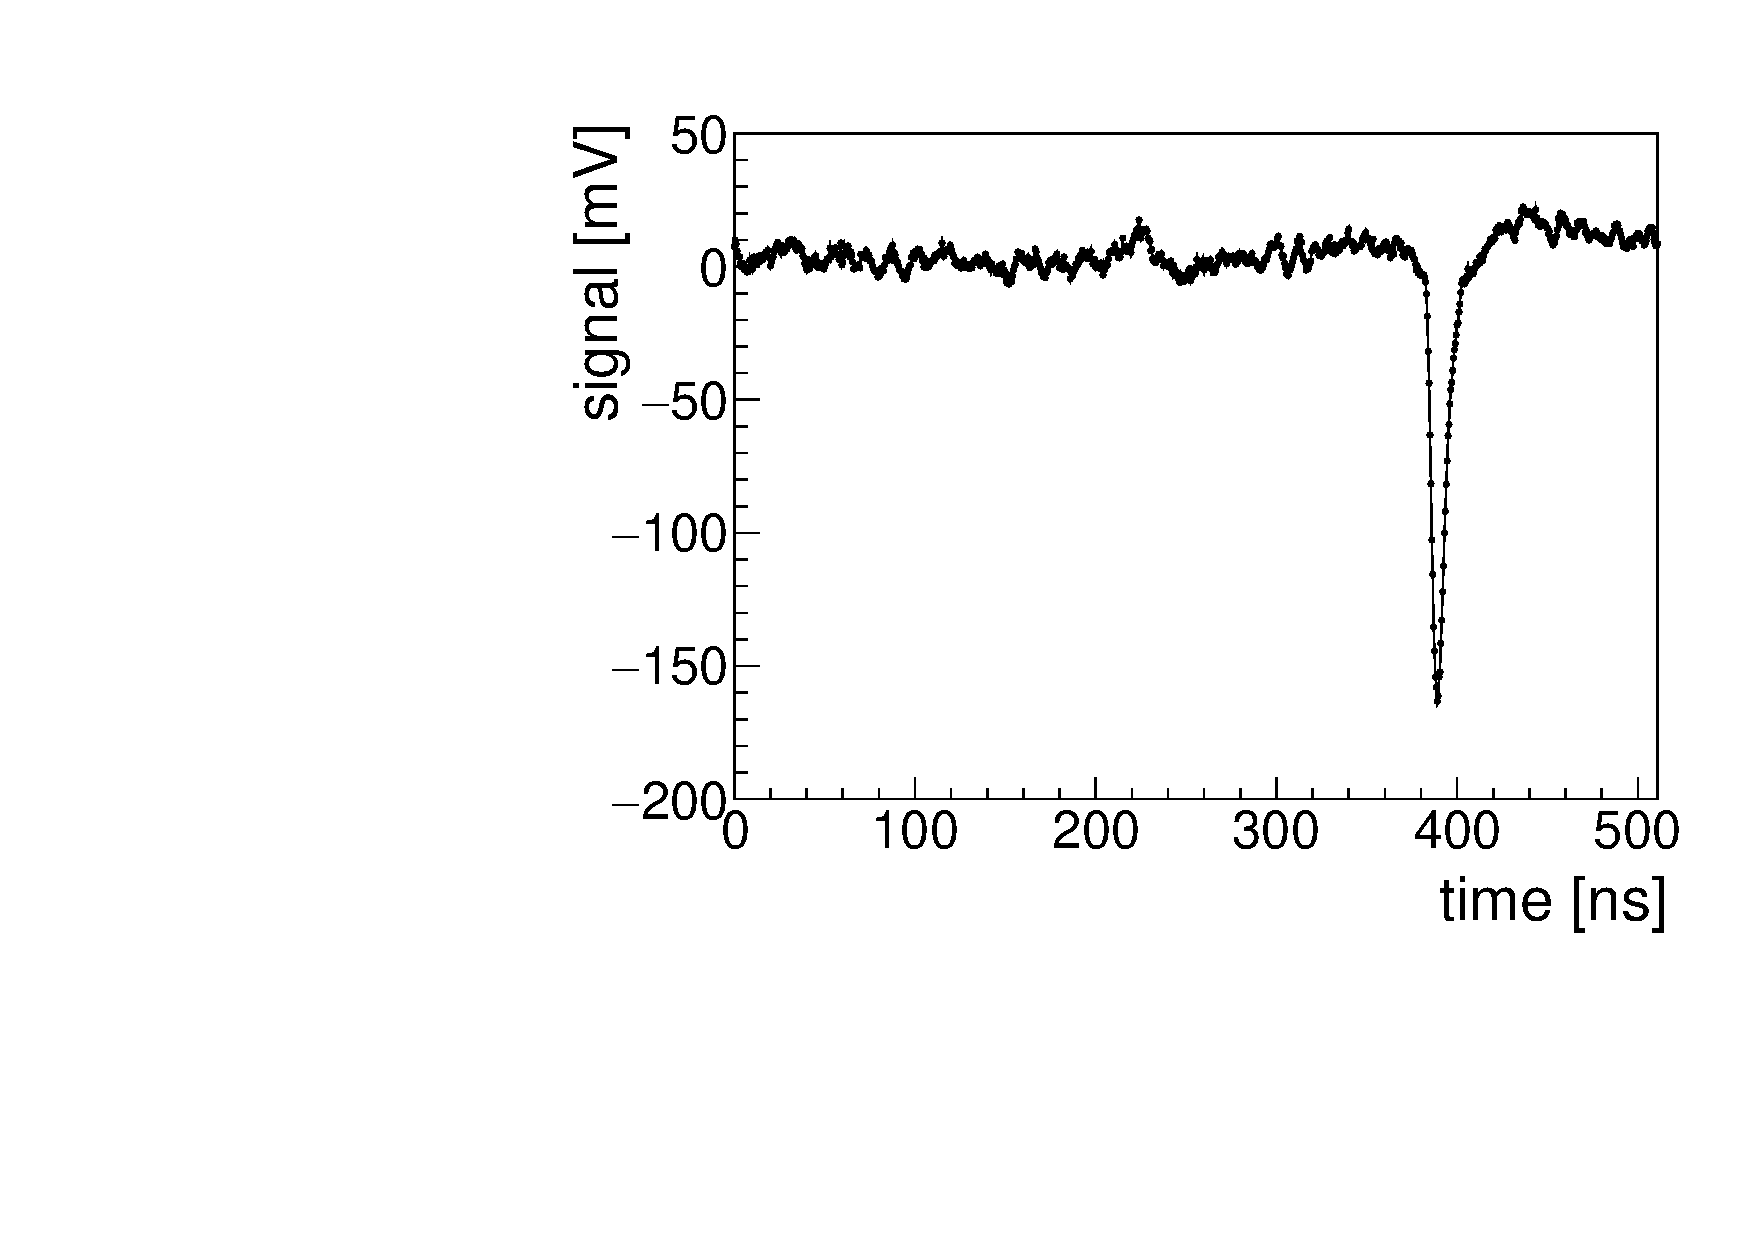
\includegraphics[angle=270, width=3.5cm]{Pul}
			\vspace*{-8pt}
			\caption{pulser waveform}
		\end{figure}
	\end{minipage}
\end{frame}
% ============================ FRAME 23 ==========================================>
\begin{frame}
	\frametitle{Cuts (2)}
	\begin{minipage}{8cm}
		\textbf{\underline{timing:}}
		\begin{itemize}
			\setlength{\itemsep}{\fill}
			\item signal peak timing follows Gaussian distribution
			\item discard events with wrong timing (more than \SI{3}{\upsigma})
			\begin{itemize}
				\item overlay from waveforms of different buckets
				\item other particles (electrons, muons)
			\end{itemize}
		\end{itemize}
		\vspace*{1cm}
		\textbf{\underline{bucket:}}
		\begin{itemize}
			\setlength{\itemsep}{\fill}
			\item two particles in consecutive buckets 
			\item first one hits the scintillator but not the diamond
			\item wrong trigger timing (\SI[retain-explicit-plus]{20}{ns})
			\item no signal in signal region
		\end{itemize}
	\end{minipage}
	\begin{minipage}{4cm}
		\vspace*{-2pt}
		\begin{figure}
			\centering
			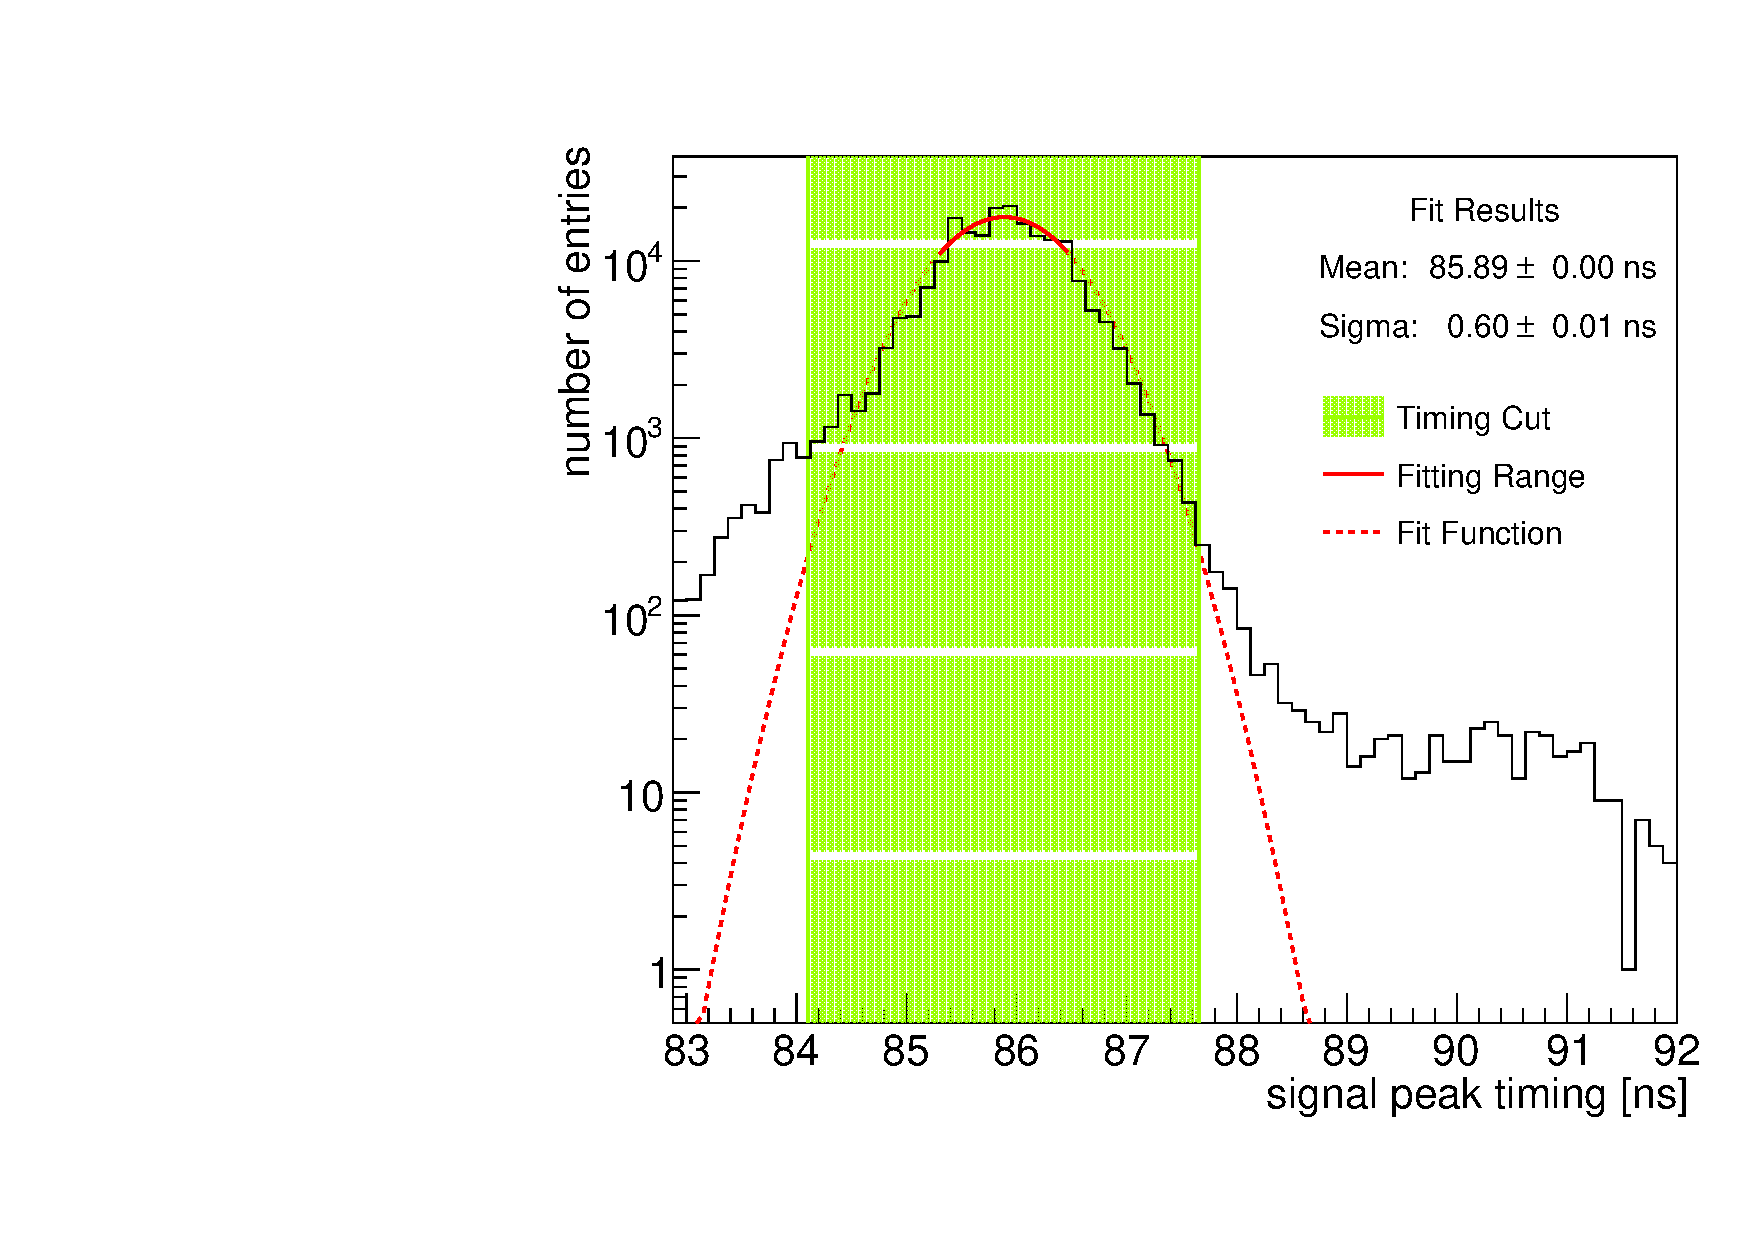
\includegraphics[angle=270, width=3.2cm]{Timing}
			\vspace*{-8pt}
			\caption{signal peak timing}
		\end{figure}
		\vspace*{-25pt}
		\begin{figure}
			\centering
			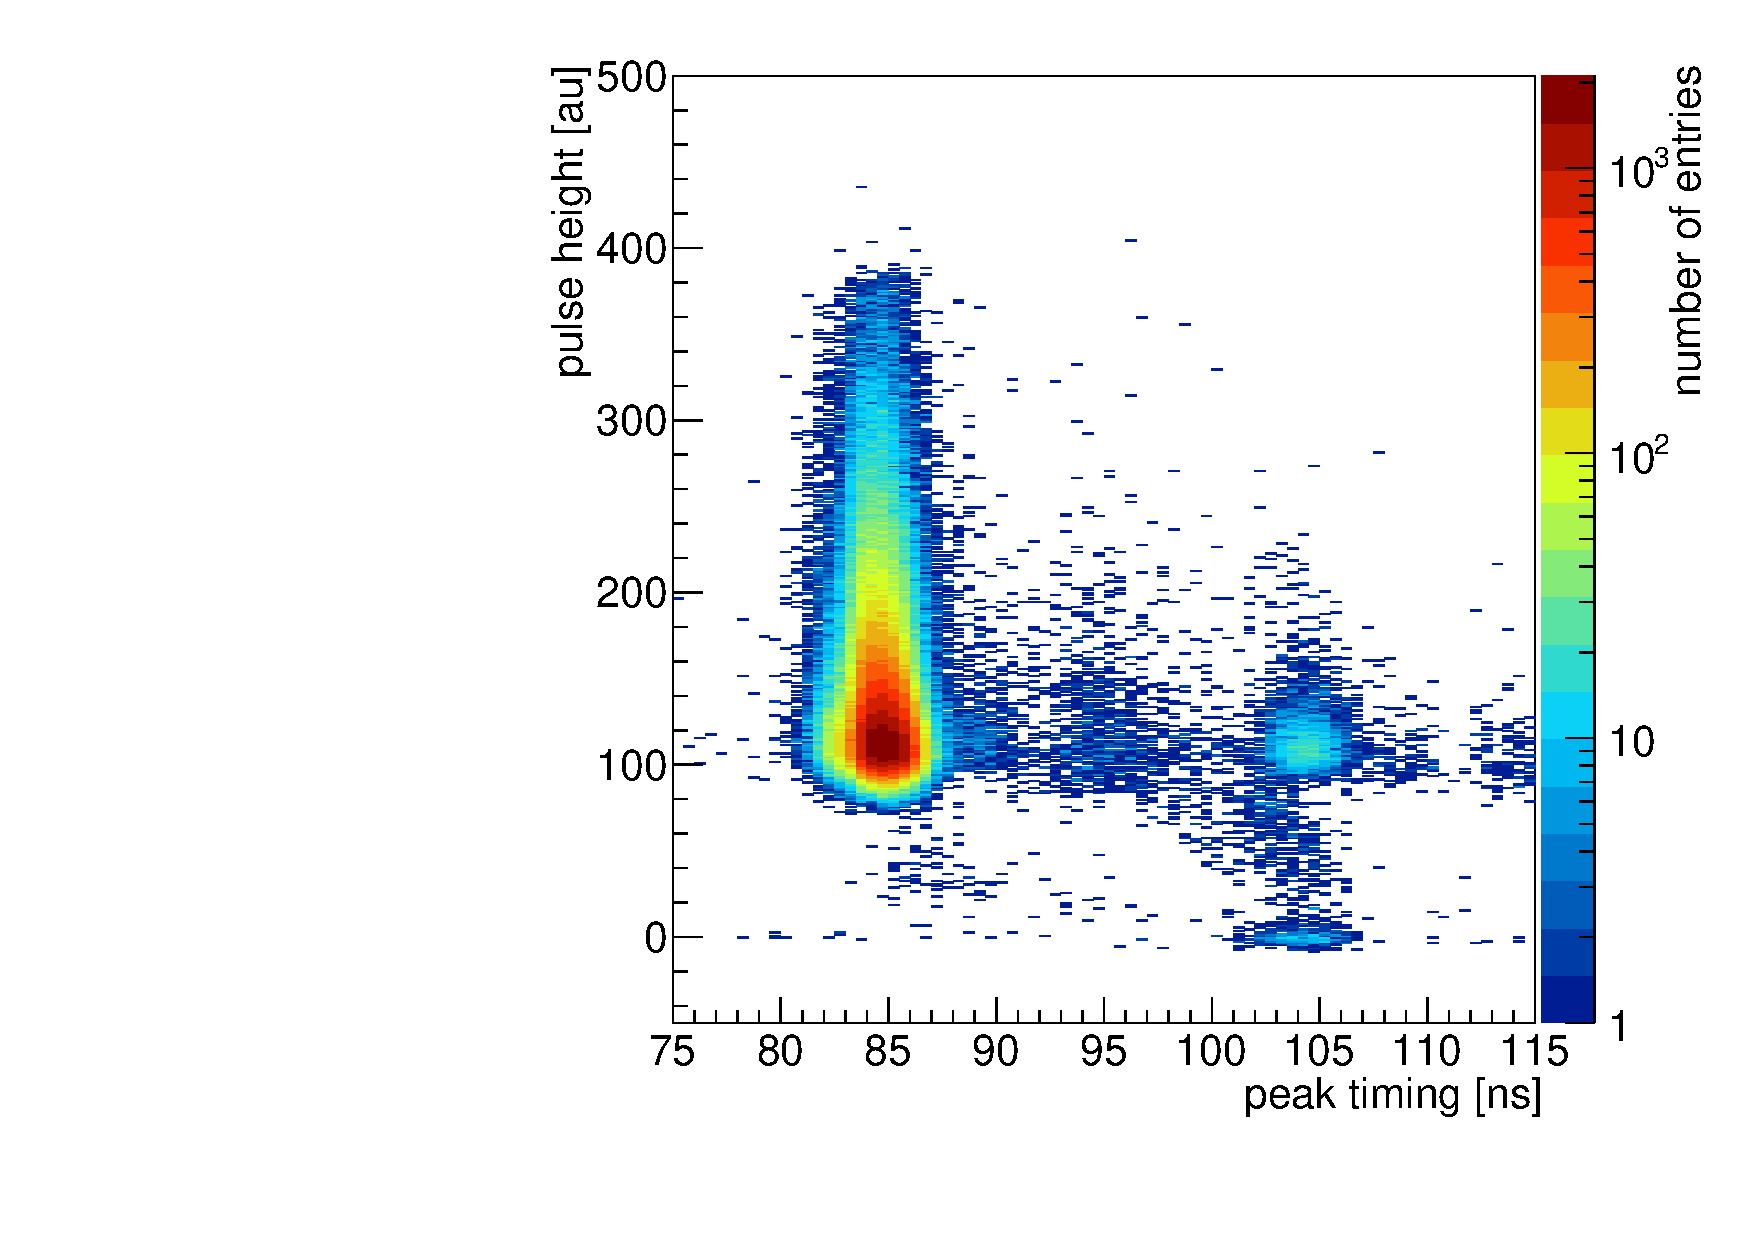
\includegraphics[angle=270, width=3.2cm]{Bucket}
			\vspace*{-8pt}
			\caption{bucket pedestal}
		\end{figure}
	\end{minipage}
\end{frame}
% ============================ FRAME 24 ==========================================>
\begin{frame}
	\frametitle{Cuts (3)}
	\begin{minipage}{8cm}
		\textbf{\underline{fiducial:}}
		\begin{itemize}
			\setlength{\itemsep}{\fill}
			\item only select uniform physical center area of the diamond 
			\item exclude edges and guard ring 
		\end{itemize}
		\vspace*{1cm}
		\textbf{\underline{other:}}
		\begin{itemize}
			\setlength{\itemsep}{\fill}
			\item $\upchi^{2}$ in $x$ and $y$ of the track fit
			\item track angle in $x$ and $y$
			\item event range
			\item beam interruptions
			\item pedestal sigma
		\end{itemize}
	\end{minipage}
	\begin{minipage}{4cm}
		\vspace*{-2pt}
		\begin{figure}
			\centering
			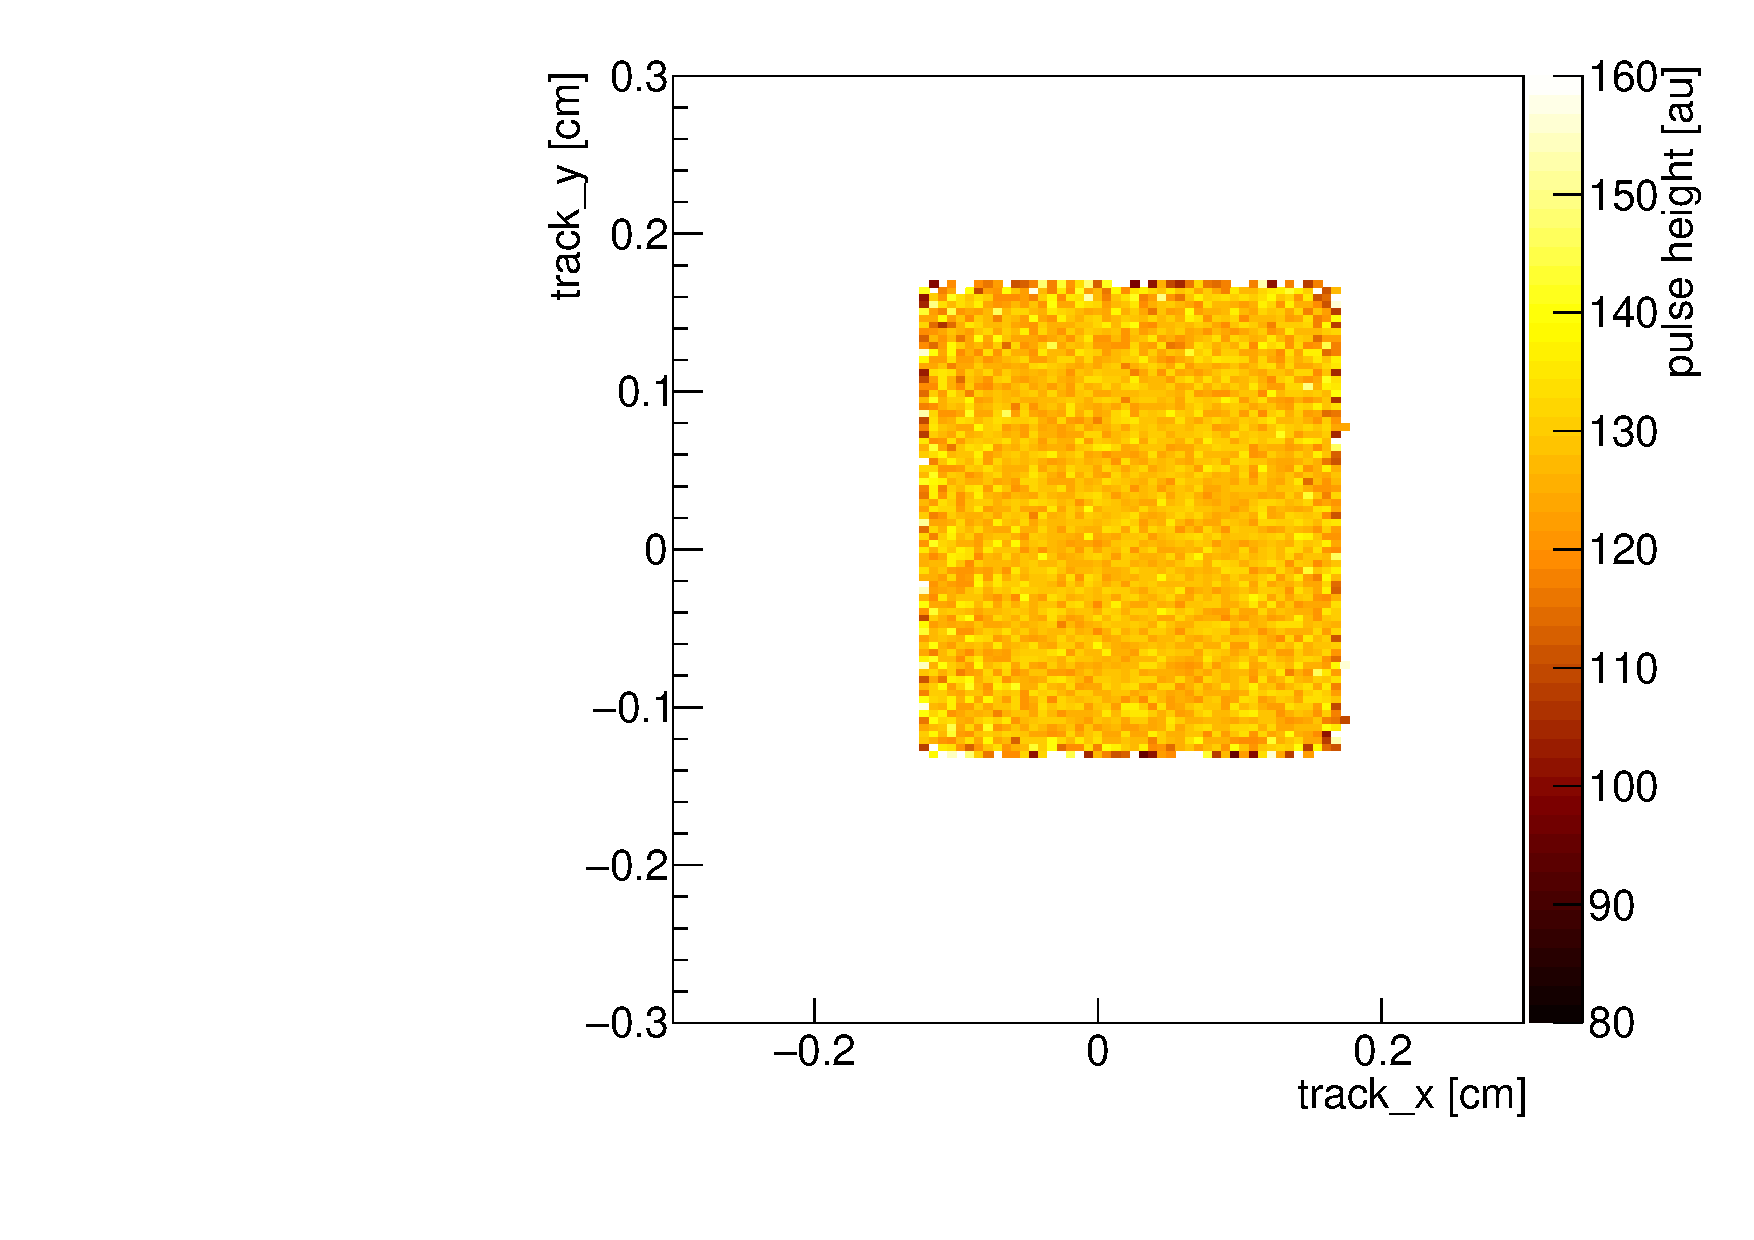
\includegraphics[angle=270, width=3.2cm]{FidNo}
			\vspace*{-8pt}
			\caption{signal map}
		\end{figure}
		\vspace*{-25pt}
		\begin{figure}
			\centering
			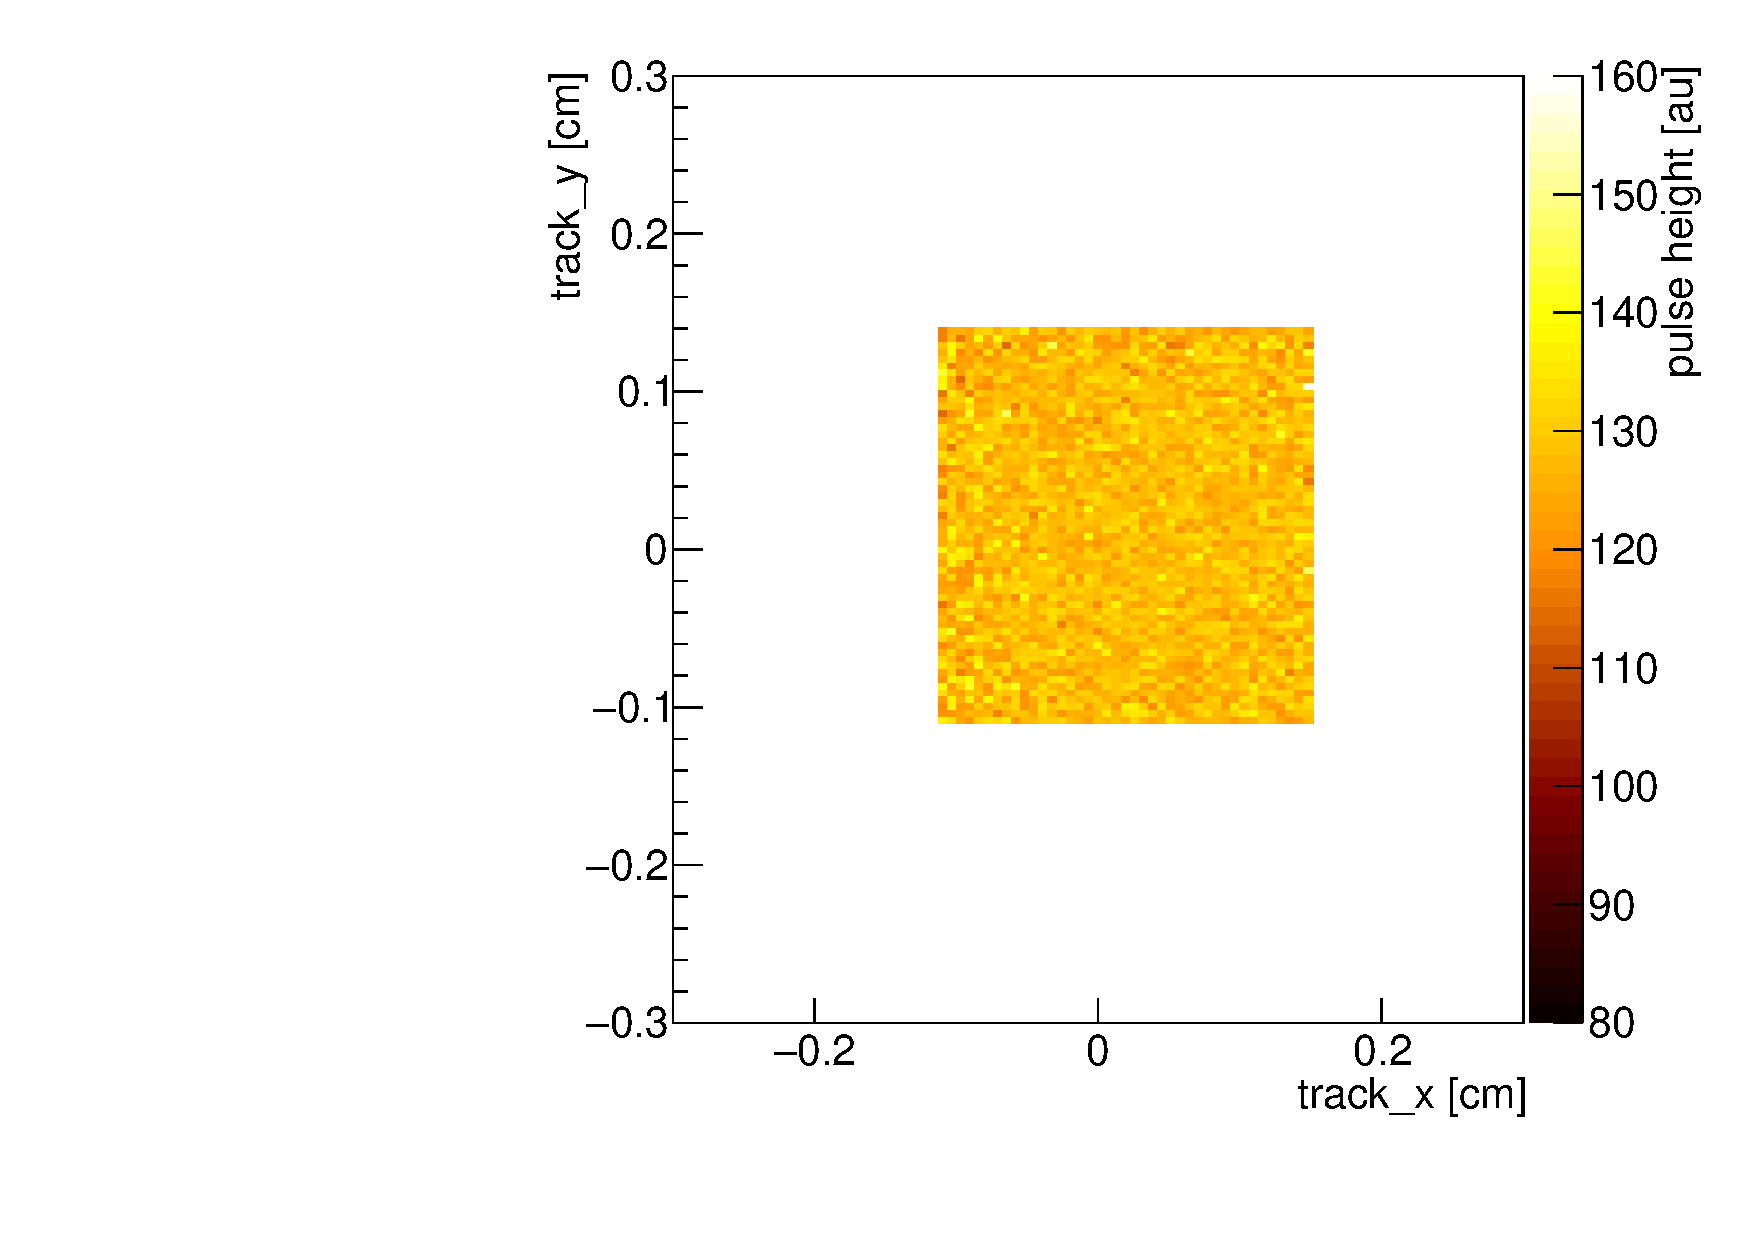
\includegraphics[angle=270, width=3.2cm]{Fid}
			\vspace*{-8pt}
			\caption{with fiducial cut}
		\end{figure}
	\end{minipage}
\end{frame}
% ============================ FRAME 25 ==========================================>
\begin{frame}
	\vspace*{-5pt}
	\begin{figure} 
		\begin{center}
			\begin{subfigure}{0.45\textwidth}  
				\centering 
				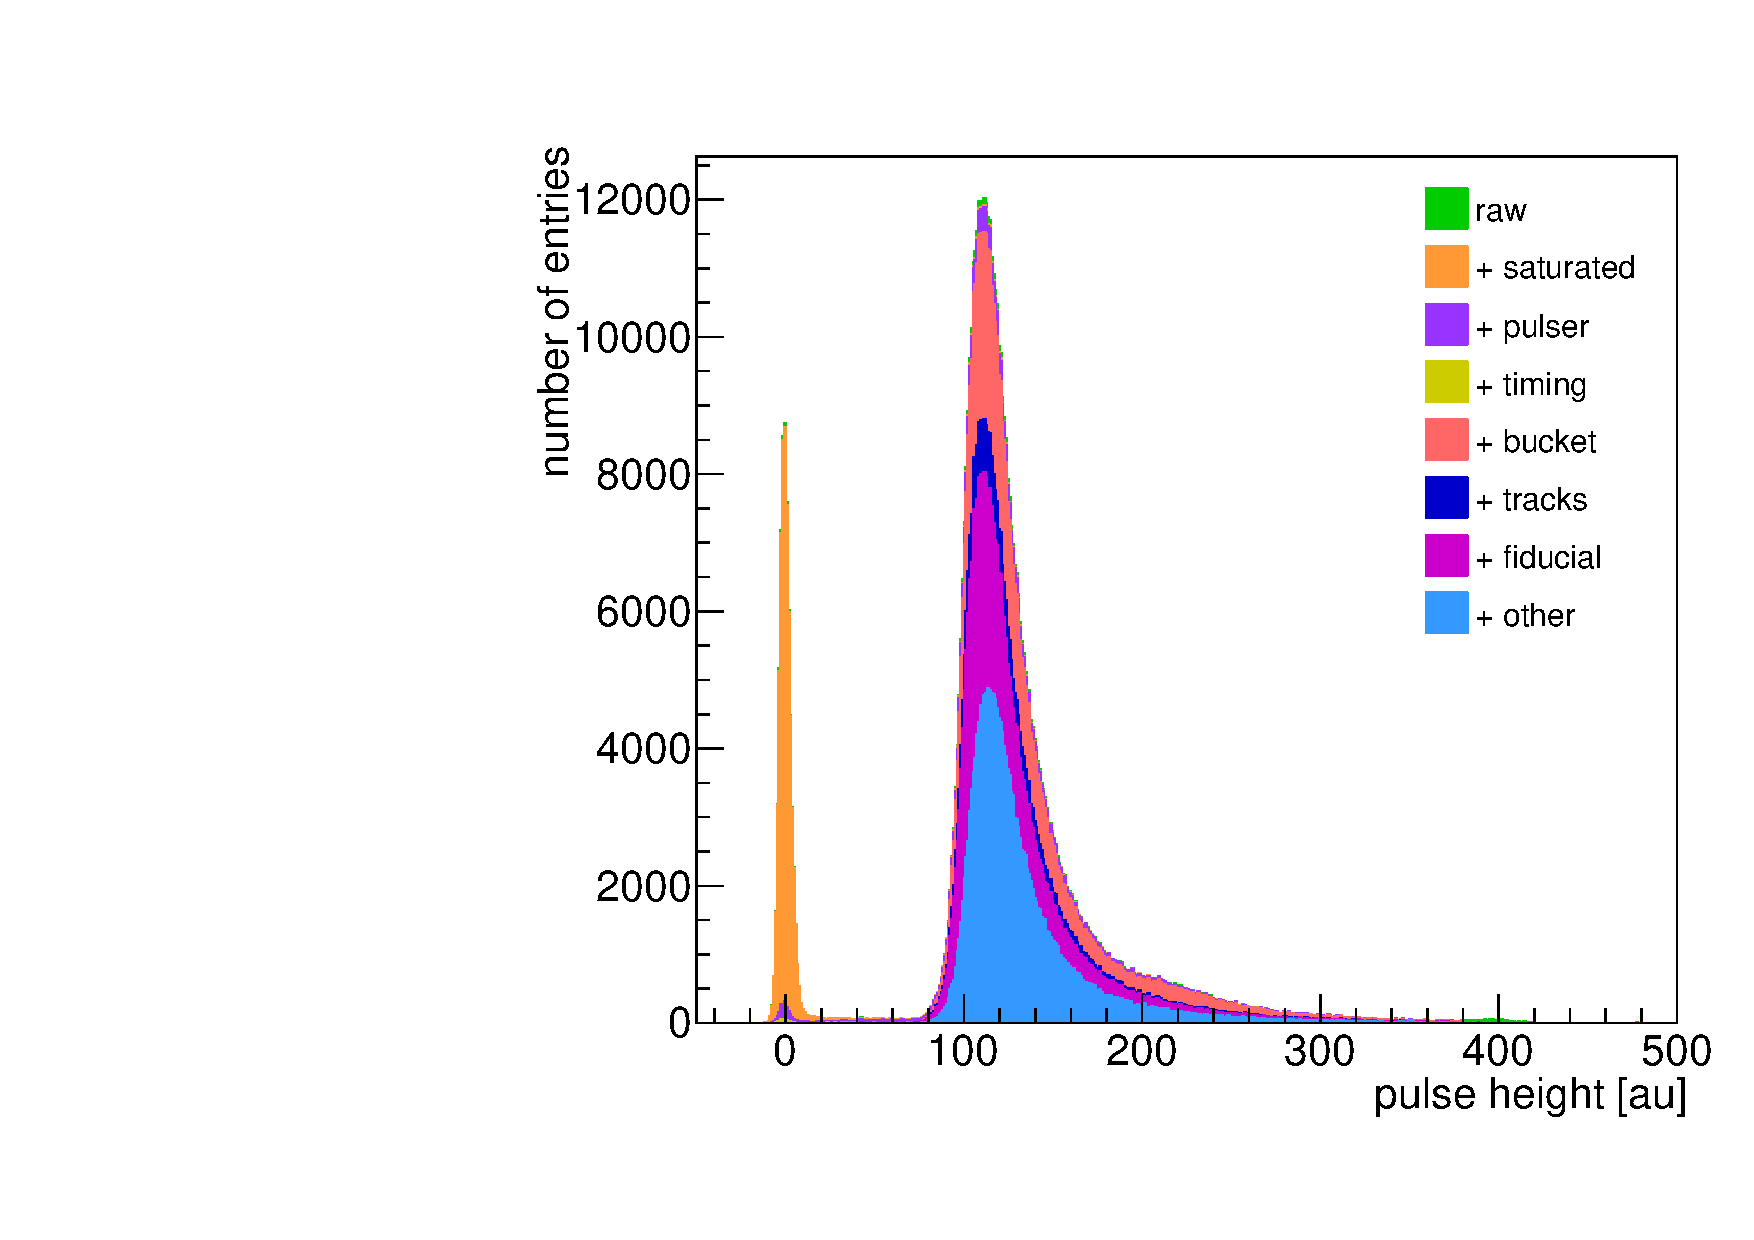
\includegraphics[angle=270, width=.85\textwidth]{Cuts}
% 				\caption{no cuts}
			\end{subfigure}
			\begin{subfigure}{0.45\textwidth} 
				\centering 
				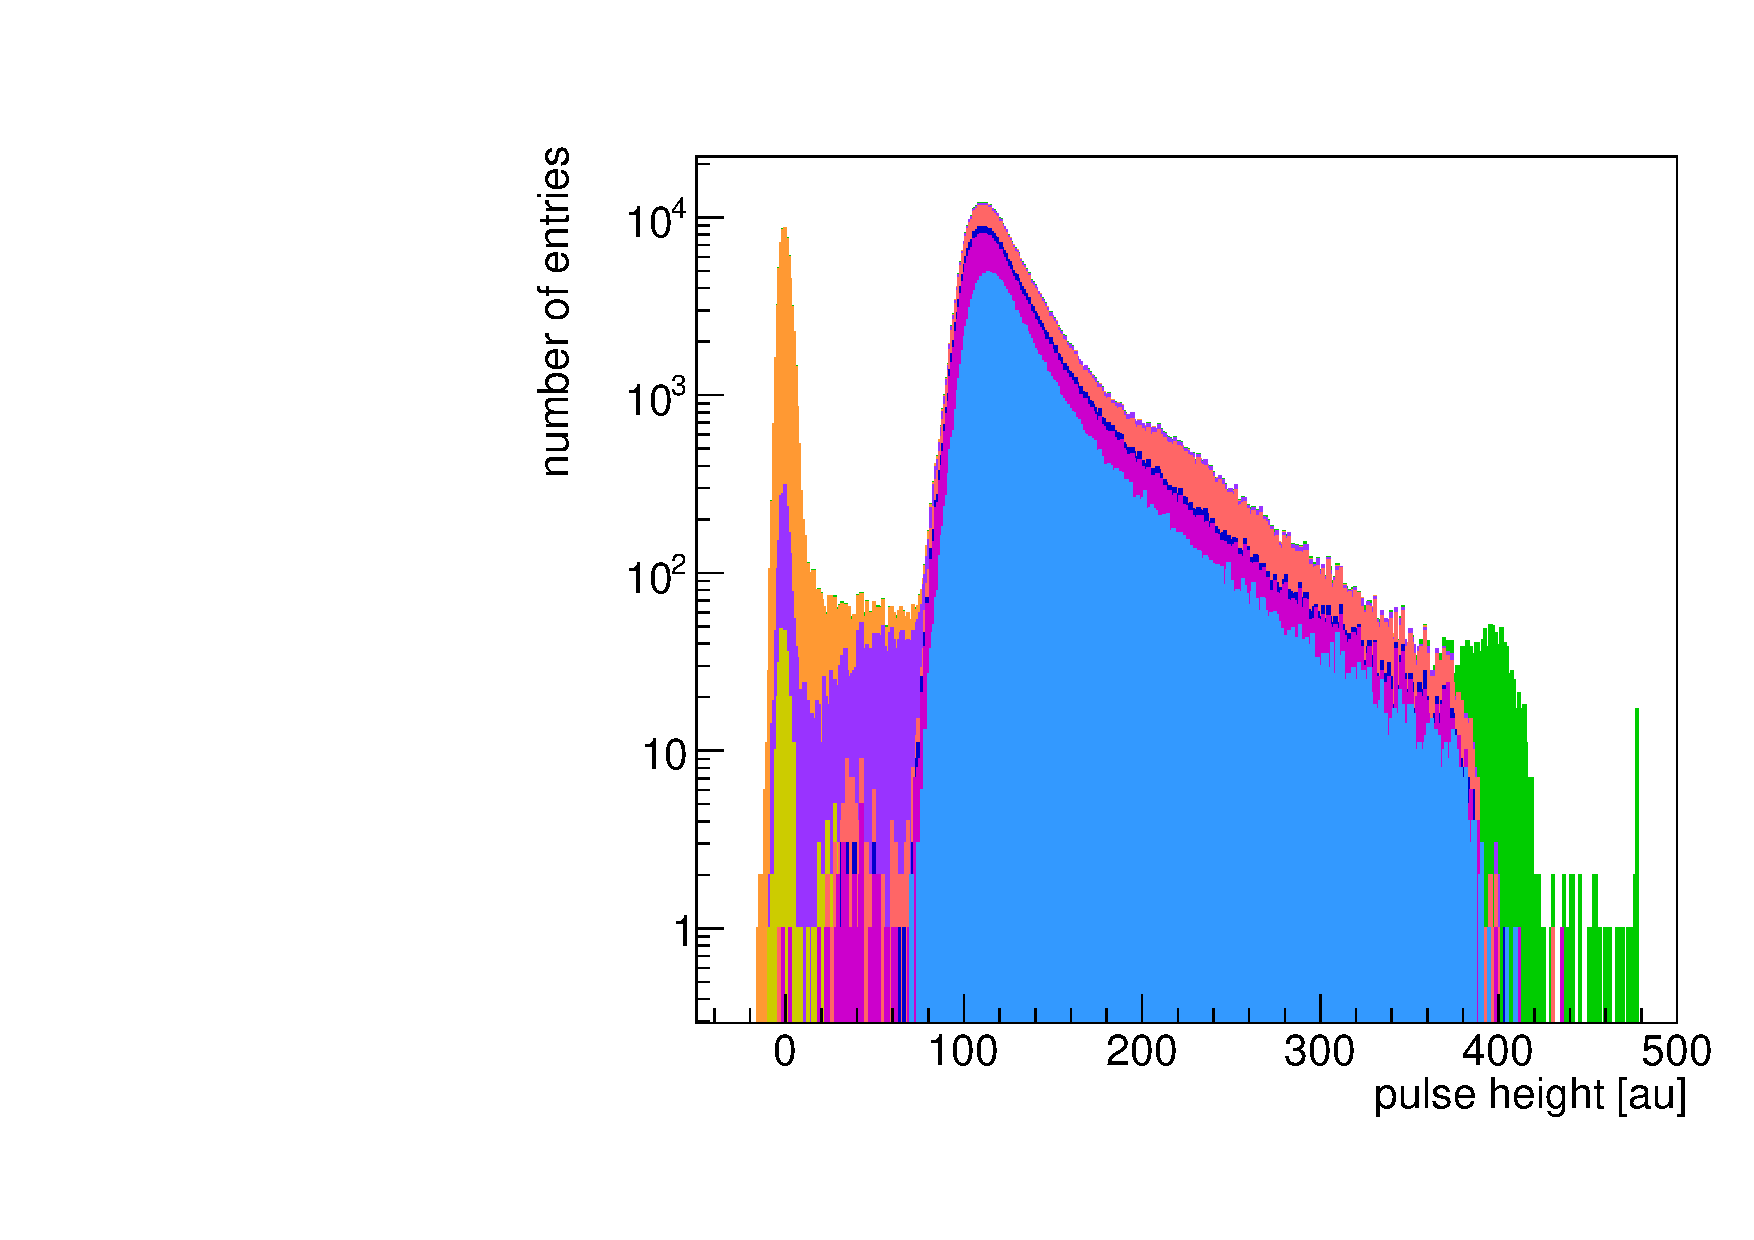
\includegraphics[angle=270, width=.85\textwidth]{CutsLog}
% 				\caption{all cuts} 	
			\end{subfigure} 
		\end{center}
	\end{figure}
	\textbf{\underline{Taken out:}}
	\begin{itemize}
		\item saturated events
		\item pedestal events (no signal)
		\item multiple hits ($\sim2$ times the signal)
		\item low signal events (guard ring, edge hits)
	\end{itemize}
\end{frame}
% ============================ FRAME 27 ==========================================>
\begin{frame}
	\frametitle{Cut Contributions}
	\begin{minipage}{4cm}
		\begin{itemize}
			\item stable pulser rate around \SIrange{10}{20}{\%}
			\item many events with incomplete or multiple tracks
			\item \SIrange{30}{40}{\%} good events after cuts
		\end{itemize}
	\end{minipage}
	\begin{minipage}{8cm}
% 		\vspace*{-17pt}
		\begin{figure}
			\centering
			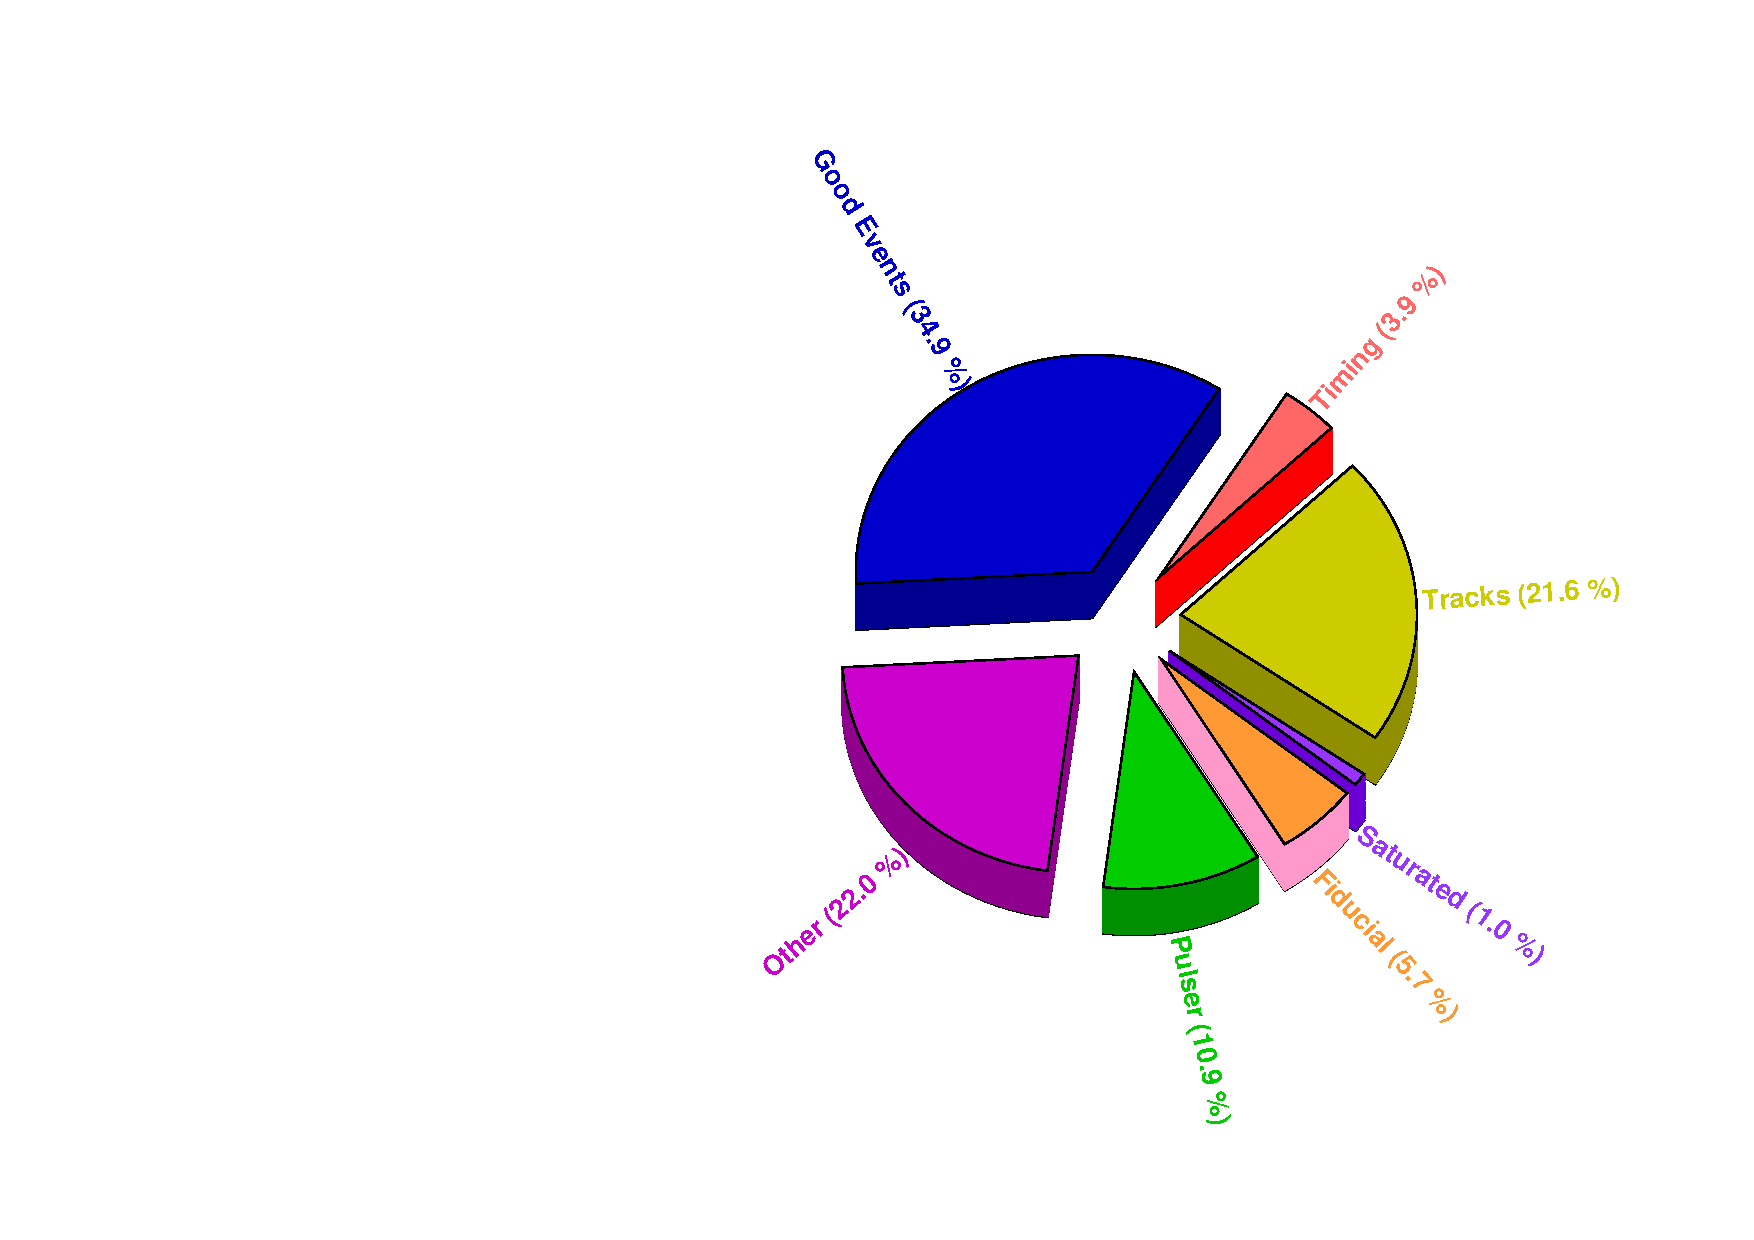
\includegraphics[angle=270, width=.9\textwidth]{CutContribution}
		\end{figure}
	\end{minipage}
\end{frame}
% ============================ FRAME 26 ==========================================>
\begin{frame}
	\frametitle{Cut Influence on the Mean Pulse Height}
	\begin{minipage}{4cm}
		\begin{itemize}
			\item very few saturated events
			\item pulser takes out pedestal events
			\item tracks discard multiple hits
		\end{itemize}
	\end{minipage}
	\begin{minipage}{8cm}
		\begin{figure}
			\centering
			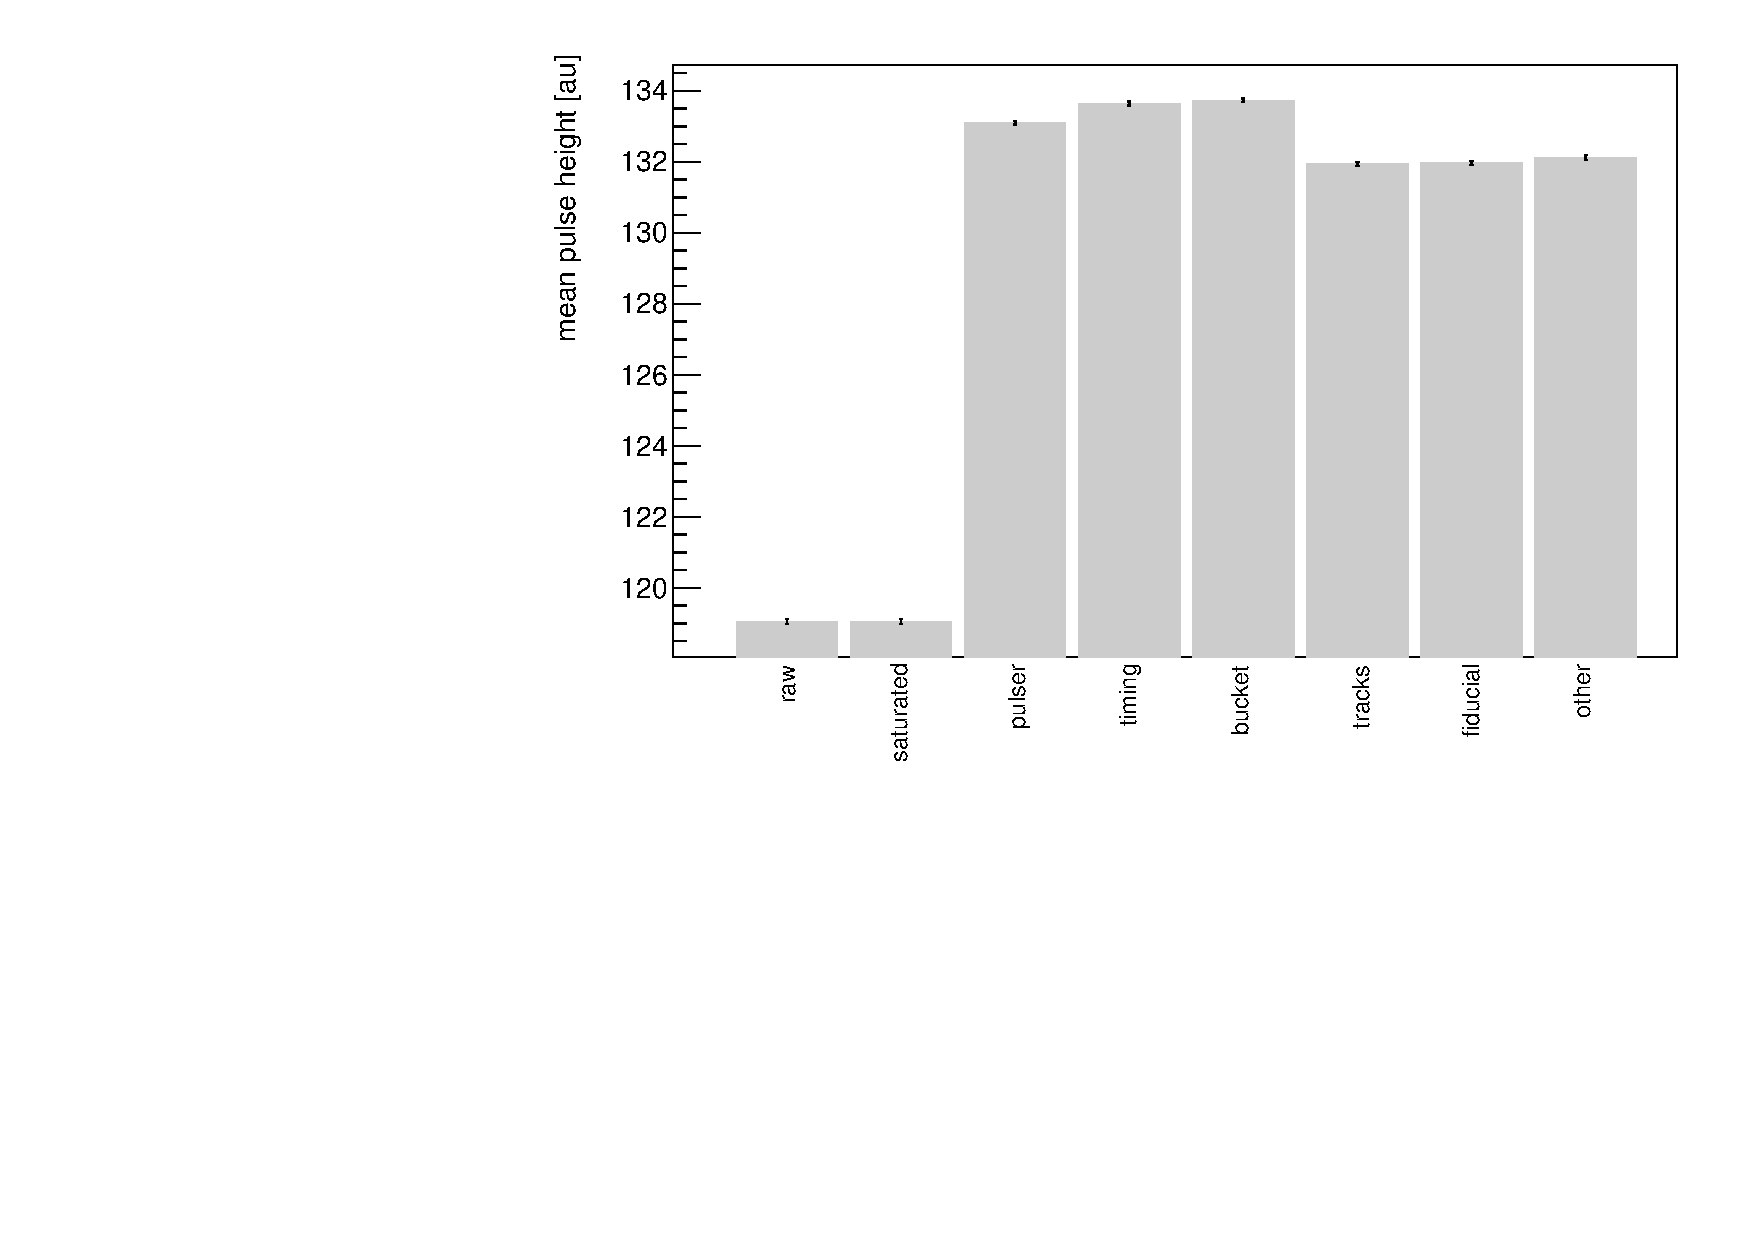
\includegraphics[angle=270, width=.9\textwidth]{CutMeans}
		\end{figure}
	\end{minipage}
\end{frame}

% END 
% BEGIN RESULTS
\subsection{Results}
% ============================ new frame ==========================================>
\begin{frame}
	\frametitle{Signal vs. Particle Flux}
	\begin{minipage}[c][.75\textheight]{.5\textwidth}
		\begin{itemize}
			\setlength{\itemsep}{\fill}
			\item after all analysis steps: look for rate dependence of pCVD diamonds
			\item found diamond pad detectors that show no or very little dependence on rate
			\item no dependence up to \SI{2e15}{neq\per cm^2}
			\item large systematic errors due to reproducibility
		\end{itemize}
		\vspace*{3pt}
		\textbf{\underline{To do:}}
		\begin{itemize}
			\setlength{\itemsep}{\fill}
			\item test higher irradiated samples
			\item improve reproducibility
			\item check the same for pixel detectors
		\end{itemize}
	\end{minipage}
	\hspace*{5pt}
	\begin{minipage}{.45\textwidth}
		\begin{figure}
			\centering
			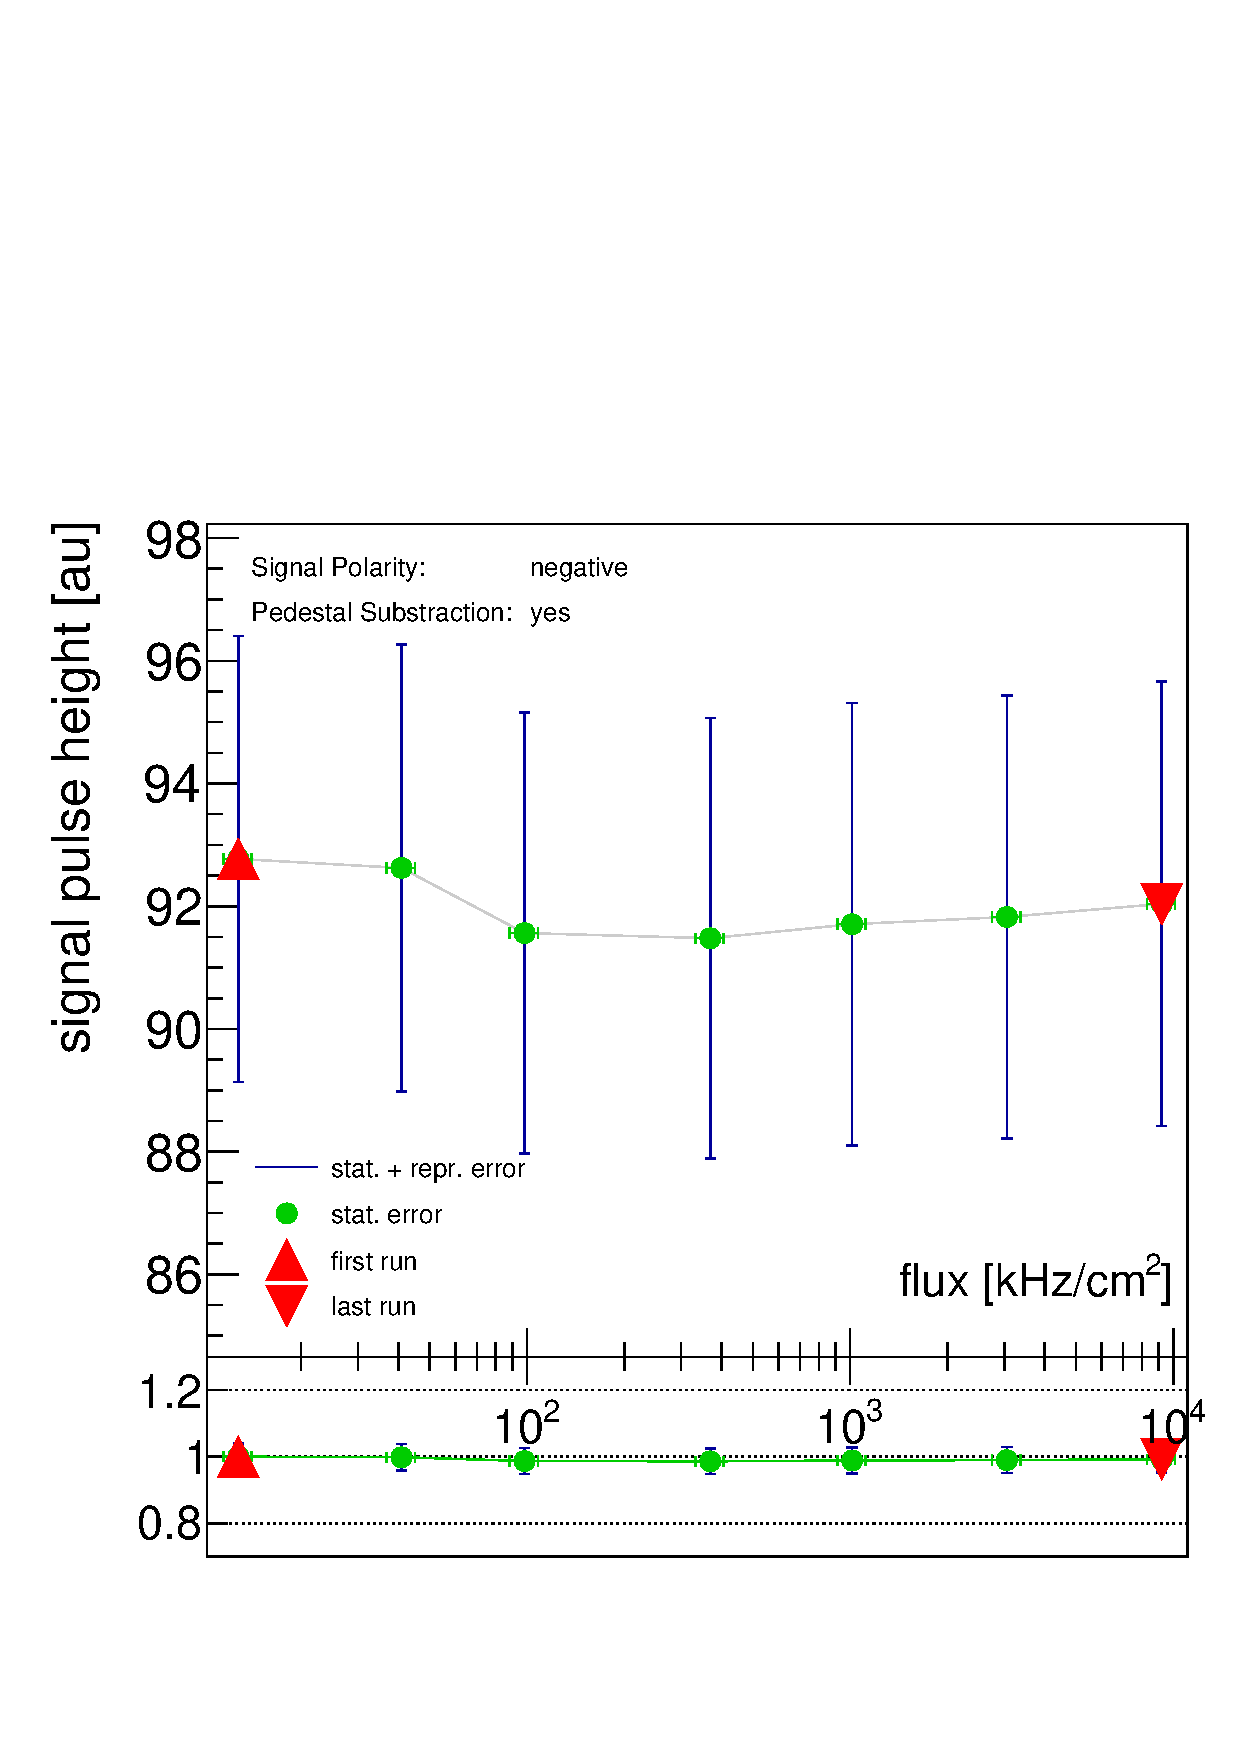
\includegraphics[width=\textwidth]{rateplot}
		\end{figure}
	\end{minipage}
\end{frame}
% ============================ new frame ==========================================>
\begin{frame}
	\frametitle{Non-Irradiated Single Crystalline Diamond}
	\def \sp {3.7cm}
	\begin{minipage}{\sp}
		\centering
		October 2015 
		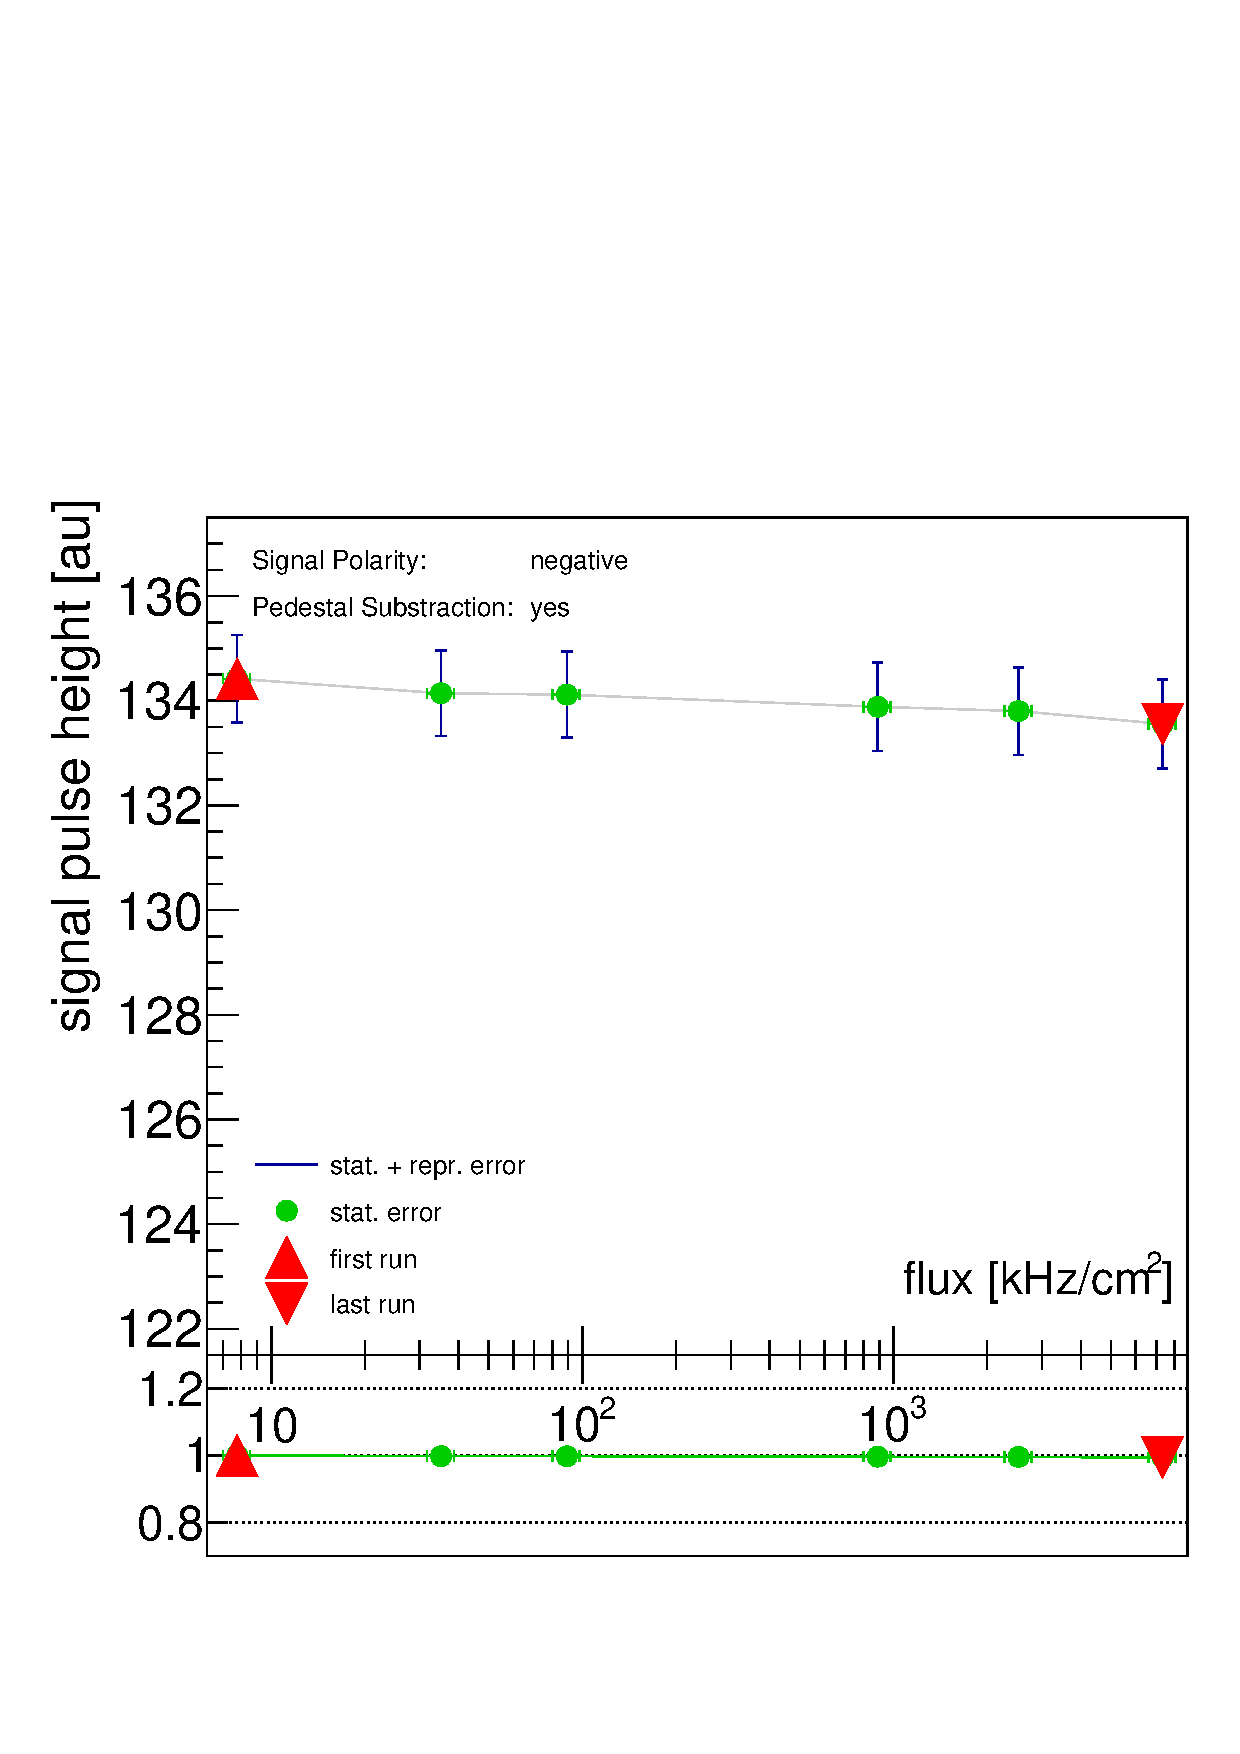
\includegraphics[width=\sp]{CPH1510_03}\\
		noise $\upsigma\approx$ \SI{2.6}{au}
	\end{minipage}
	\hspace*{2pt}
	\begin{minipage}{\sp}
		\centering
		August 2016
		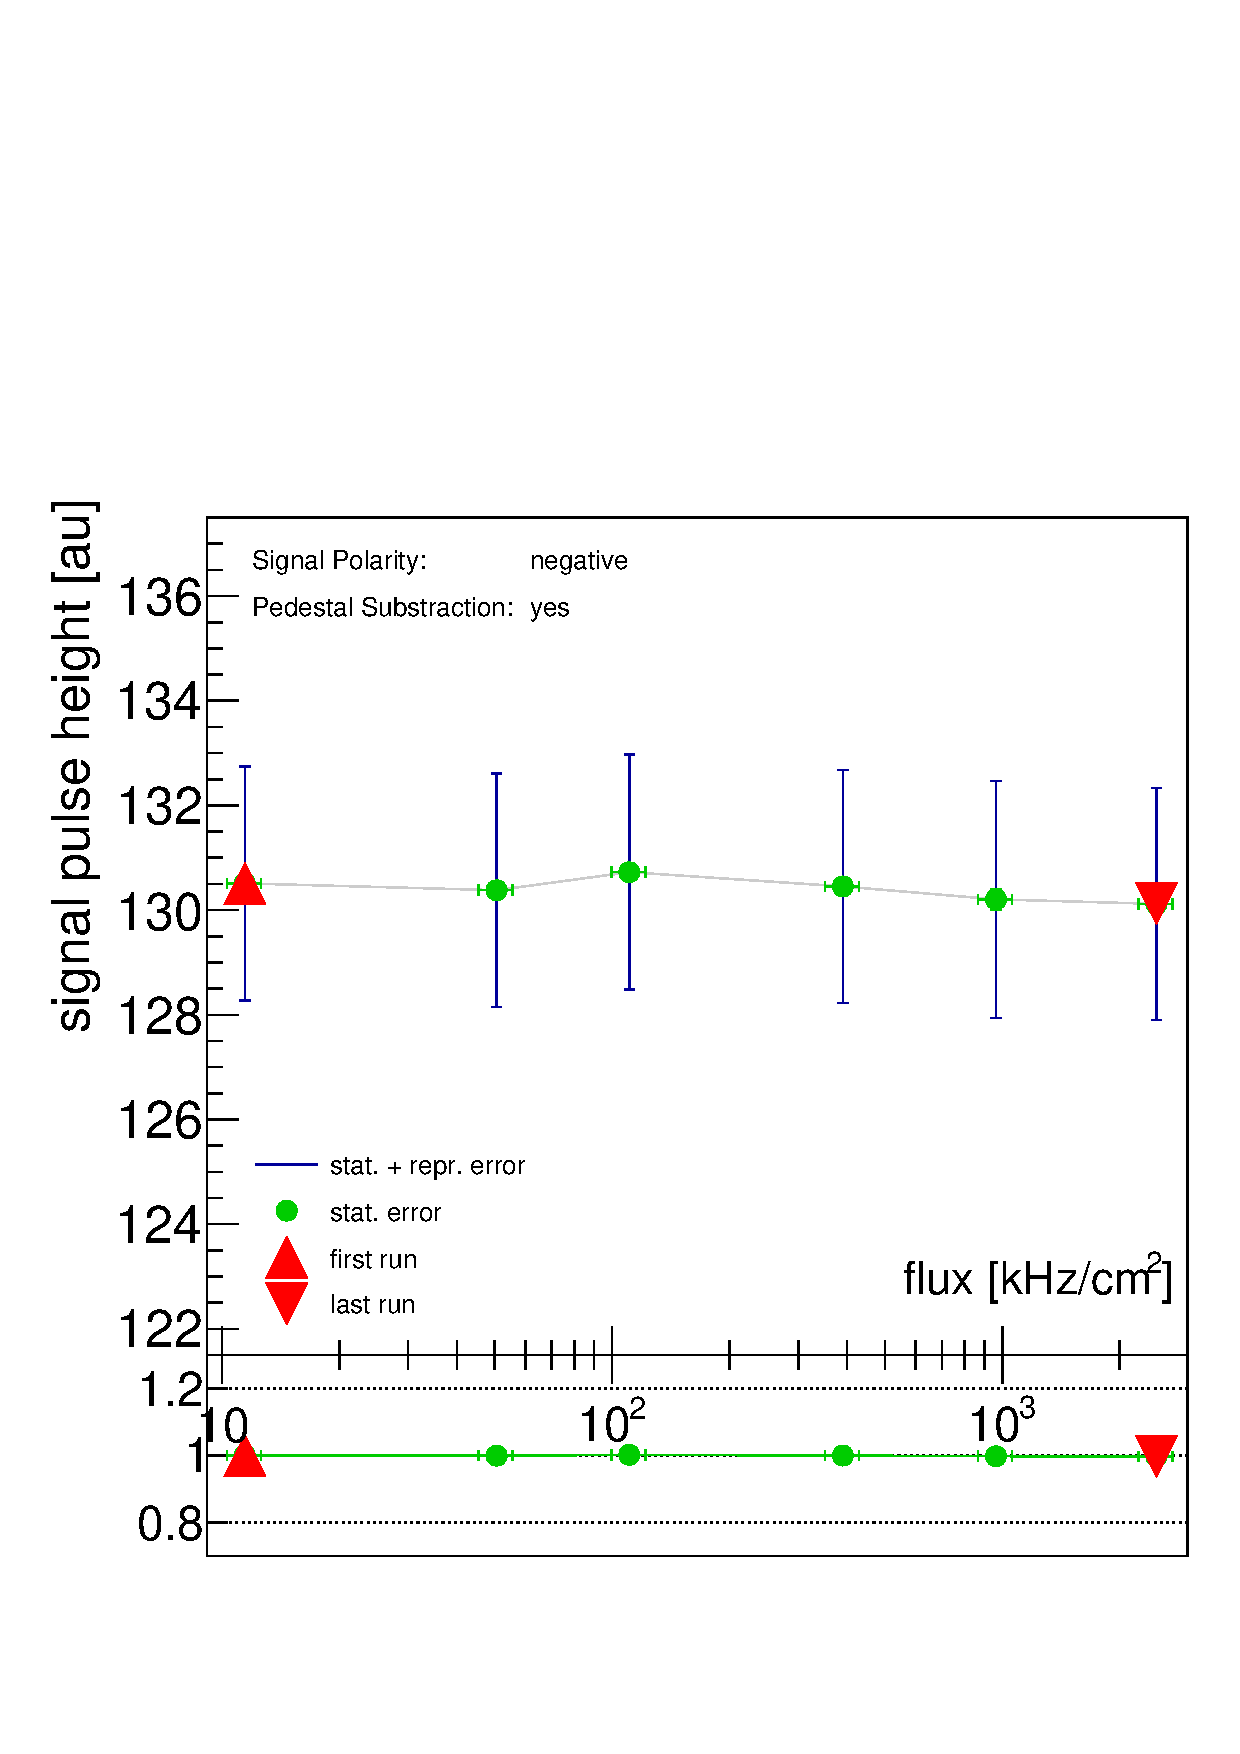
\includegraphics[width=\sp]{CPH1608_8_1}\\
		noise $\upsigma\approx$ \SI{2.6}{au}
	\end{minipage}
	\hspace*{2pt}
	\begin{minipage}{\sp}
		\centering
		October 2016
		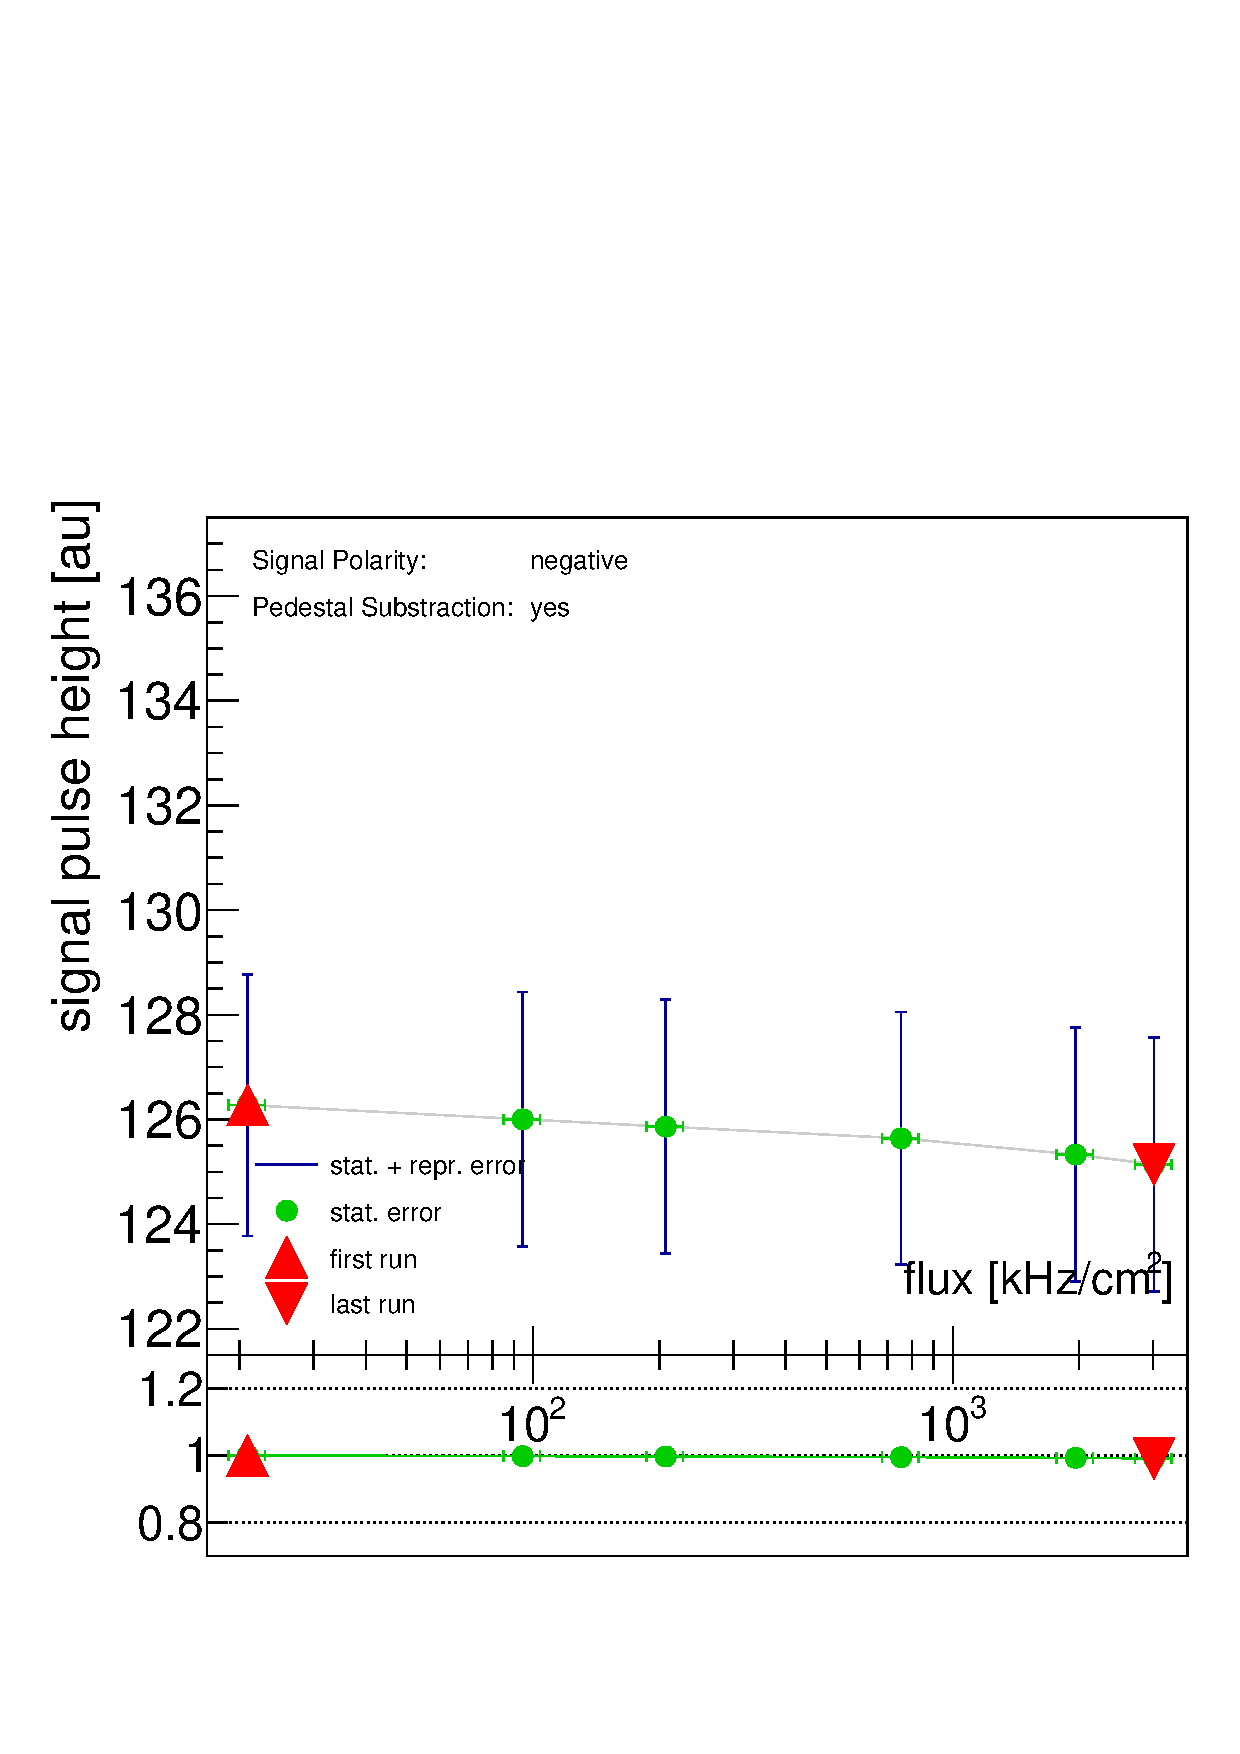
\includegraphics[width=\sp]{CPH1610_8_1}\\
		noise $\upsigma \approx$ \SI{2.6}{au}
	\end{minipage}\s
	\begin{itemize}
		\item measurements taken under the same conditions
		\item noise stays the same
		\item pulse height very stable
	\end{itemize}
\end{frame}
% ============================ new frame ==========================================>
\begin{frame}
	\frametitle{Poly crystalline diamond}
	\begin{minipage}{2.8cm}
		\centering
		August 2016 - \\unirradiated
		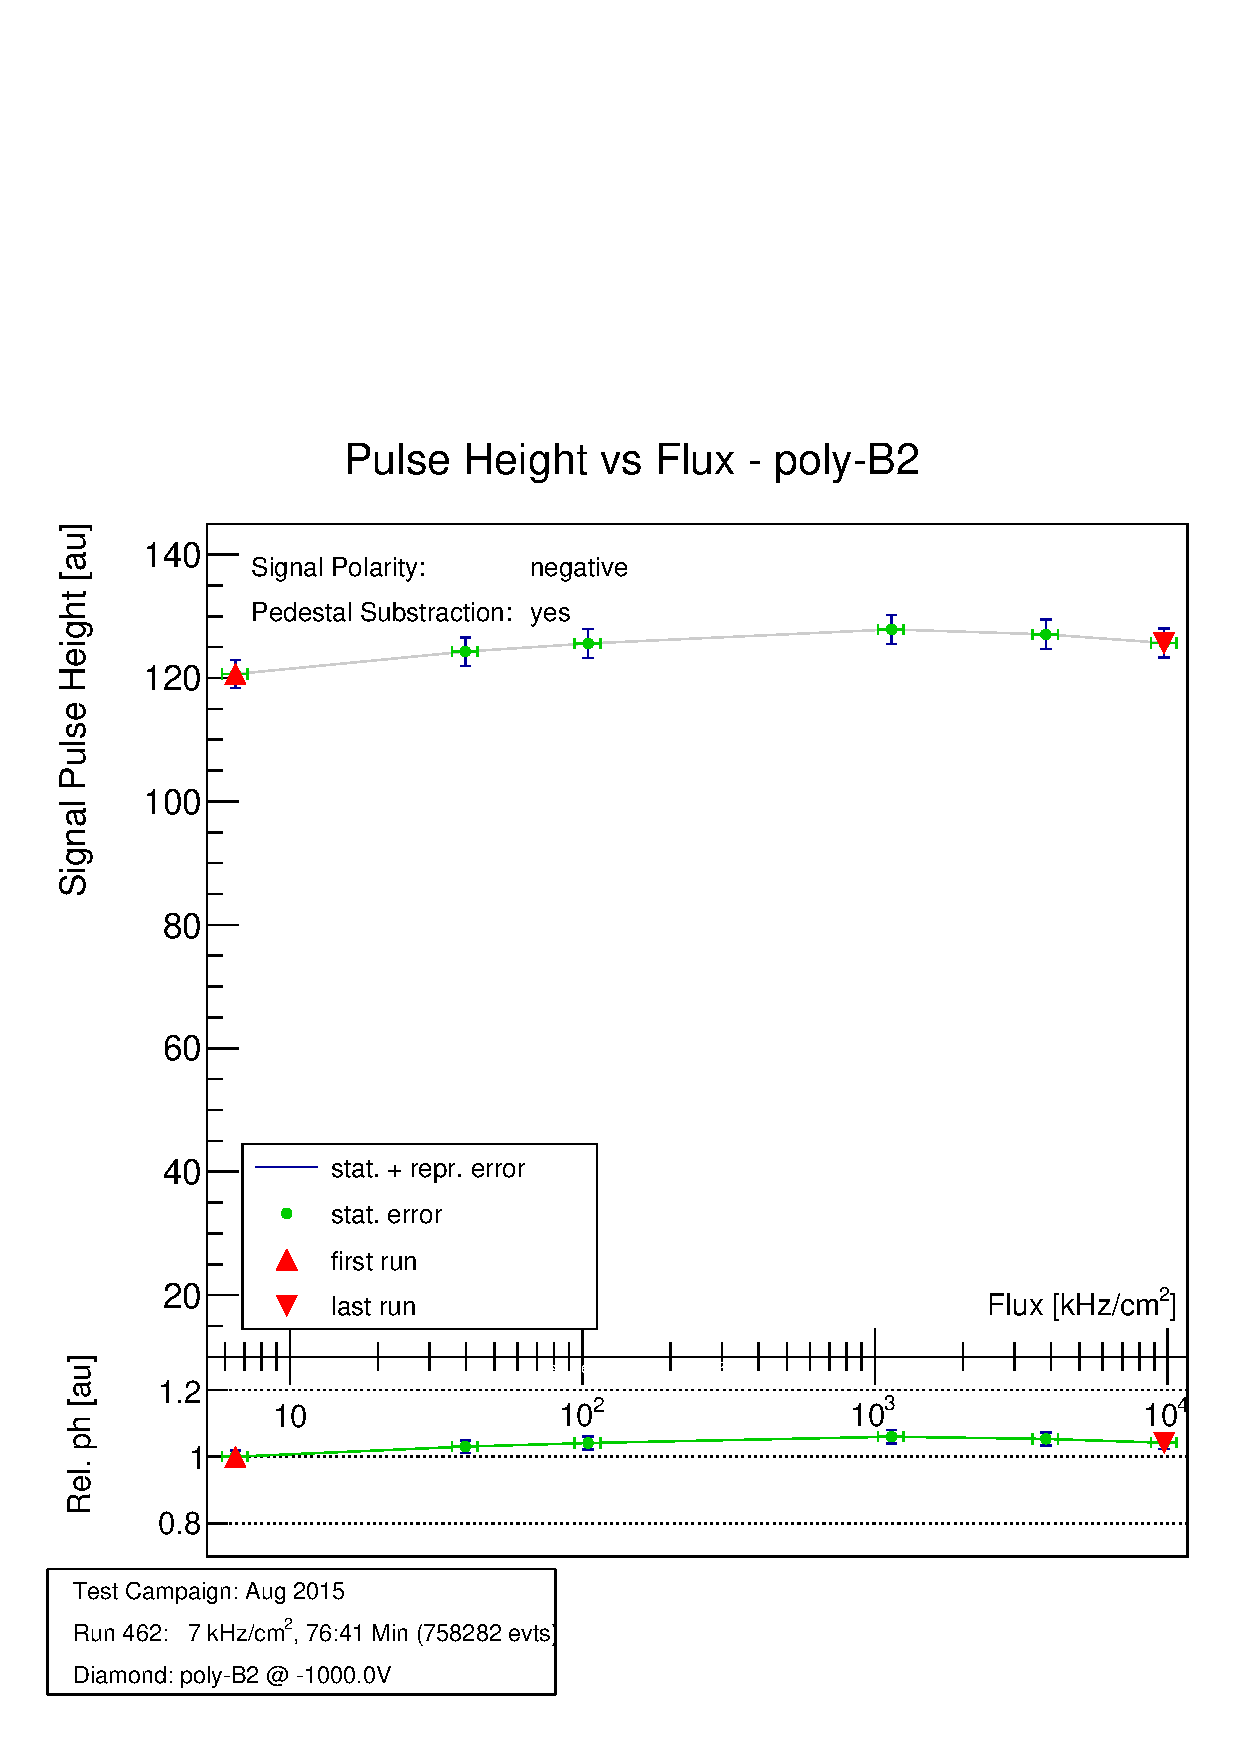
\includegraphics[width=3cm]{CPH1508_13_2.pdf}\\
		noise $\upsigma\approx$ \SI{4.9}{au}
	\end{minipage}
	\hspace*{2pt}
	\begin{minipage}{2.8cm}
		\centering
		October 2015 - \SI[exponent-product = \cdot]{5e14}{n/cm^{2}}
		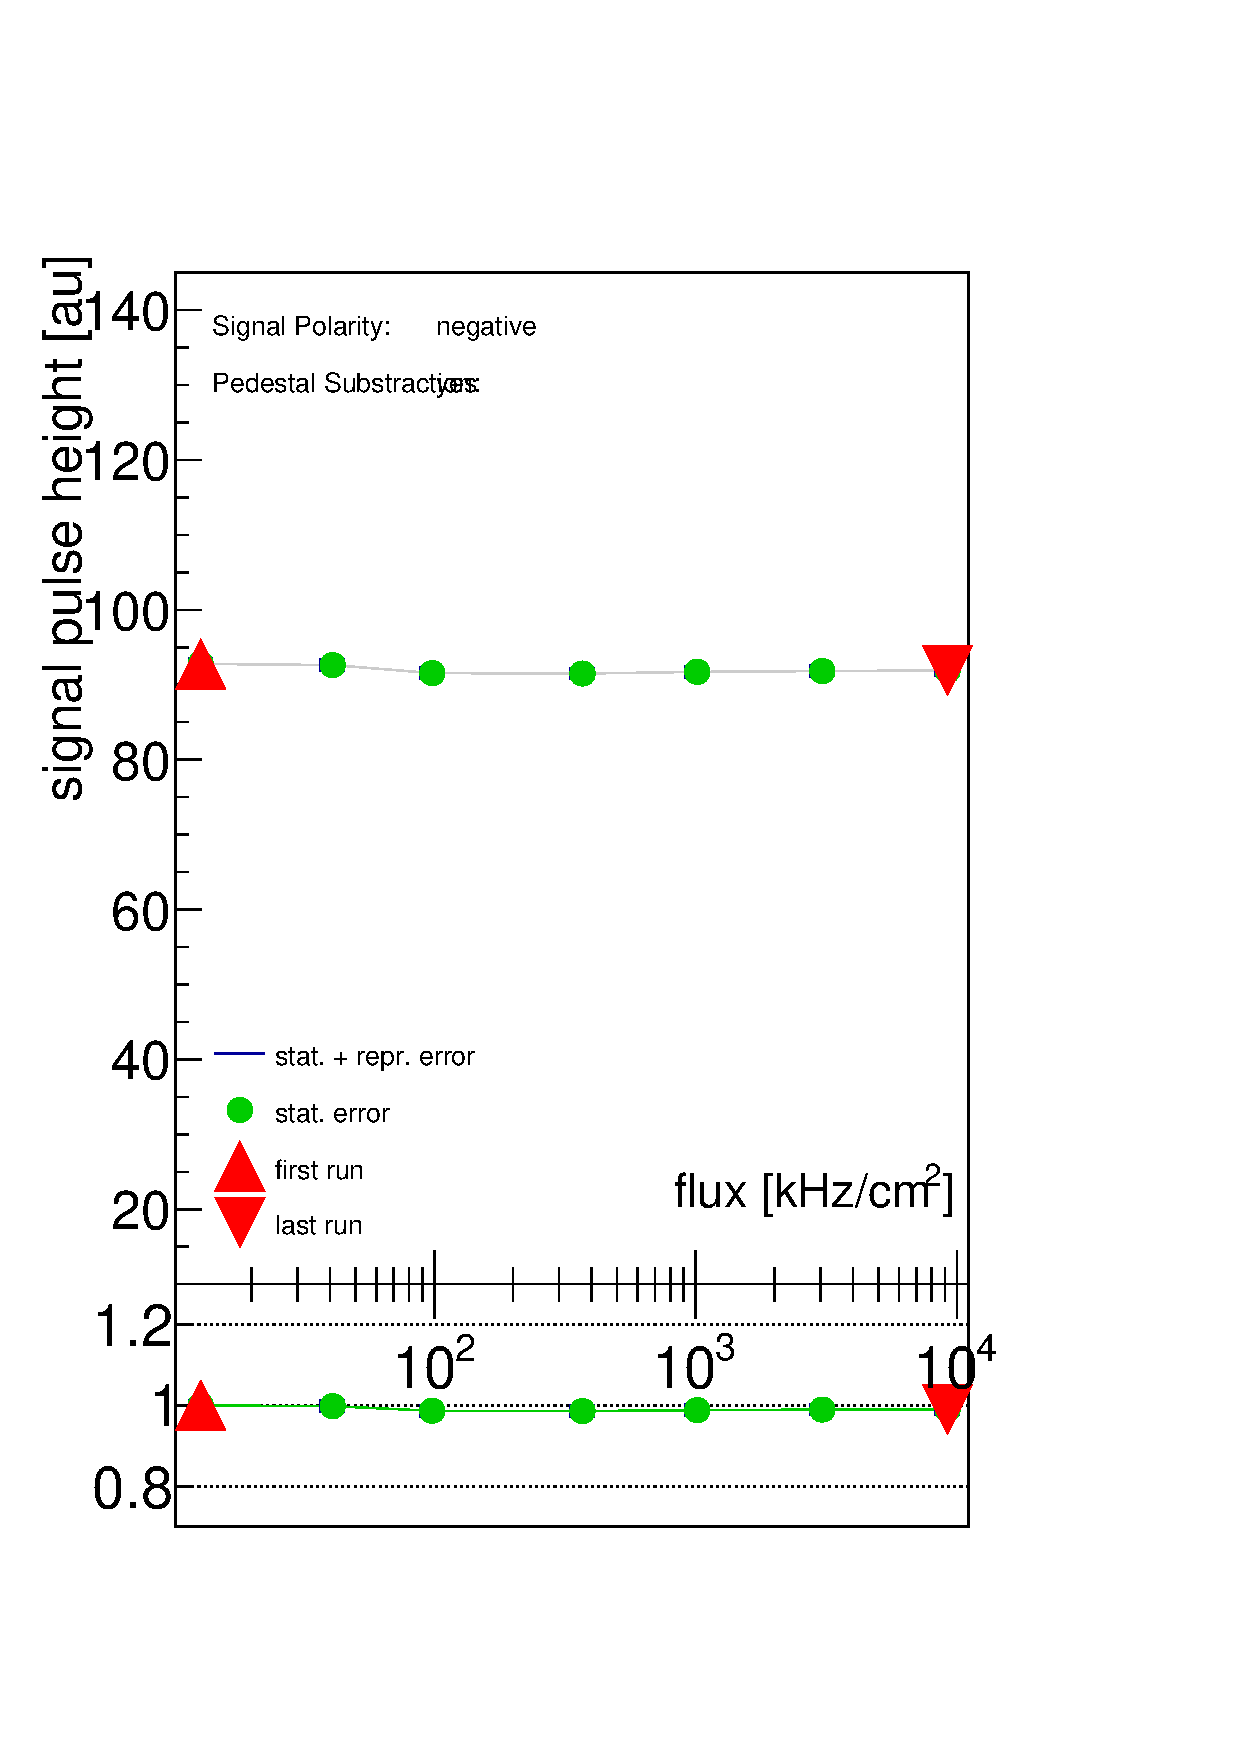
\includegraphics[width=3cm]{CPH1510_08_2.pdf}\\
		noise $\upsigma\approx$ \SI{4.9}{au}
	\end{minipage}
	\hspace*{2pt}
	\begin{minipage}{2.8cm}
		\centering
		August 2016 - \SI[exponent-product = \cdot]{1e15}{n/cm^{2}}
		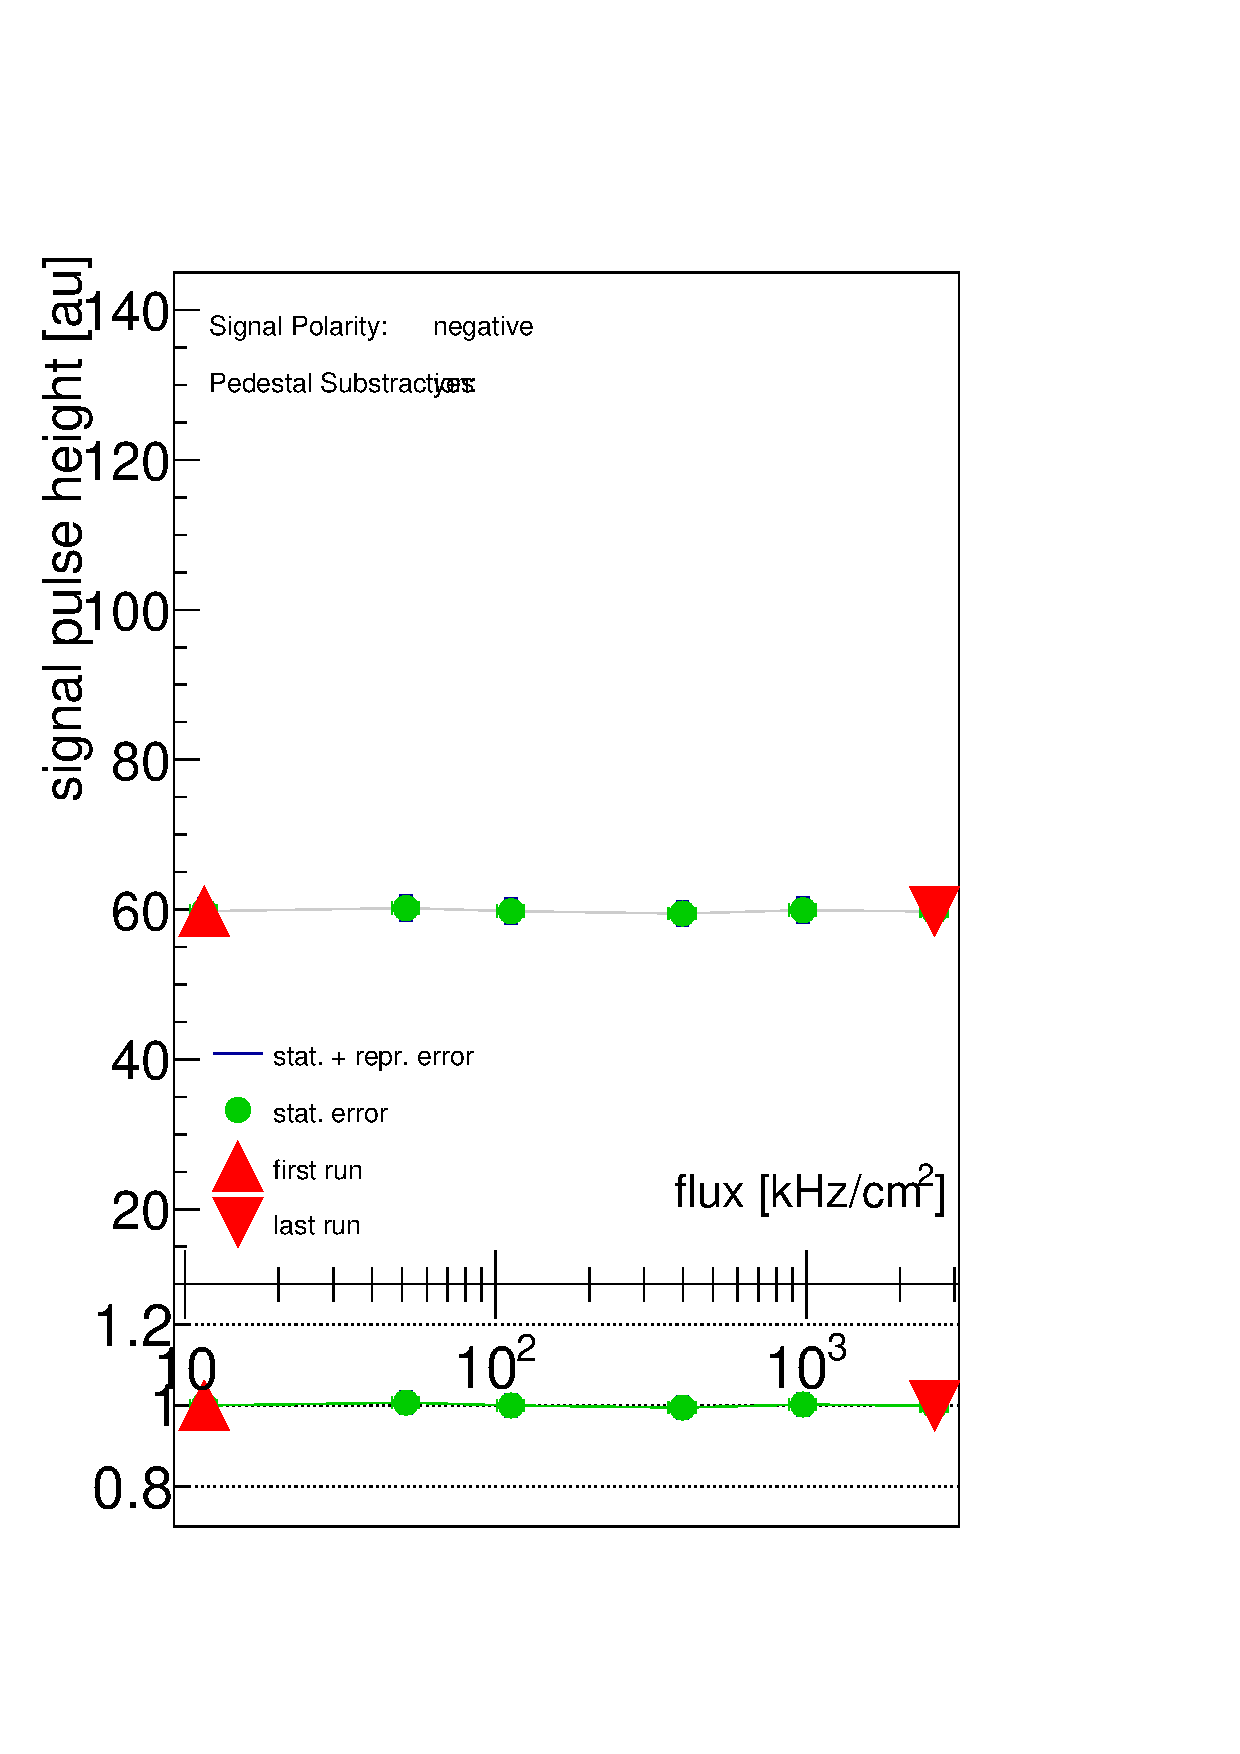
\includegraphics[width=3cm]{CPH1608_09_1.pdf}\\
		noise $\upsigma \approx$ \SI{4.9}{au}
	\end{minipage}
	\hspace*{2pt}
	\begin{minipage}{2.8cm}
		\centering
		October 2016 - \SI[exponent-product = \cdot]{2e15}{n/cm^{2}}
		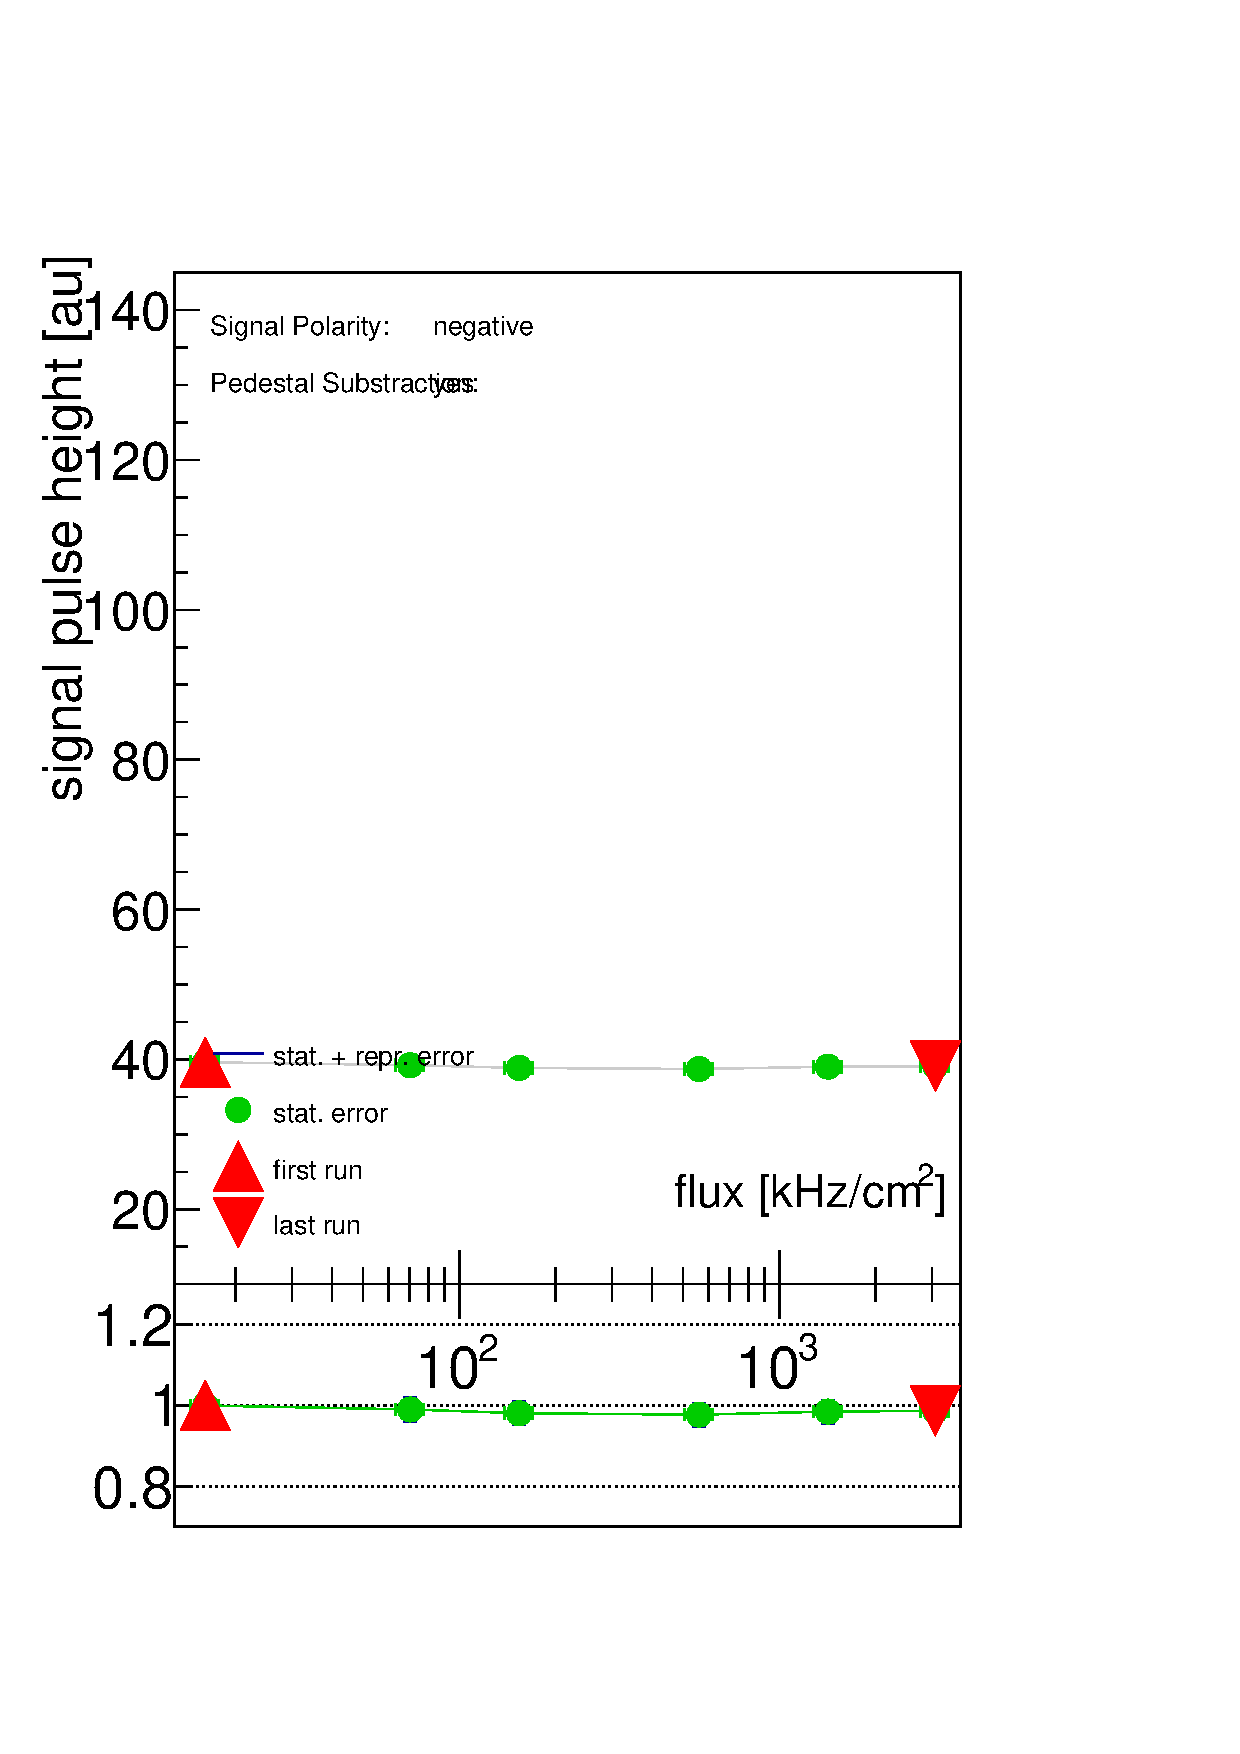
\includegraphics[width=3cm]{CPH1610_6_1.pdf}\\
		noise $\upsigma \approx$ \SI{4.9}{au}
	\end{minipage}\s
	\begin{itemize}
		\item pulse height very stable after irradiation
		\item noise stays the same
	\end{itemize}
\end{frame}
% ============================ FRAME 31 ==========================================>
\begin{frame}
	\frametitle{Pulse Height Distribution and Signal Maps}
	\vspace*{-7.5pt}
	\def \sp {0.62\textwidth}
	\begin{figure}
		\centering
		\begin{subfigure}{0.45\textwidth} 
			\centering 
			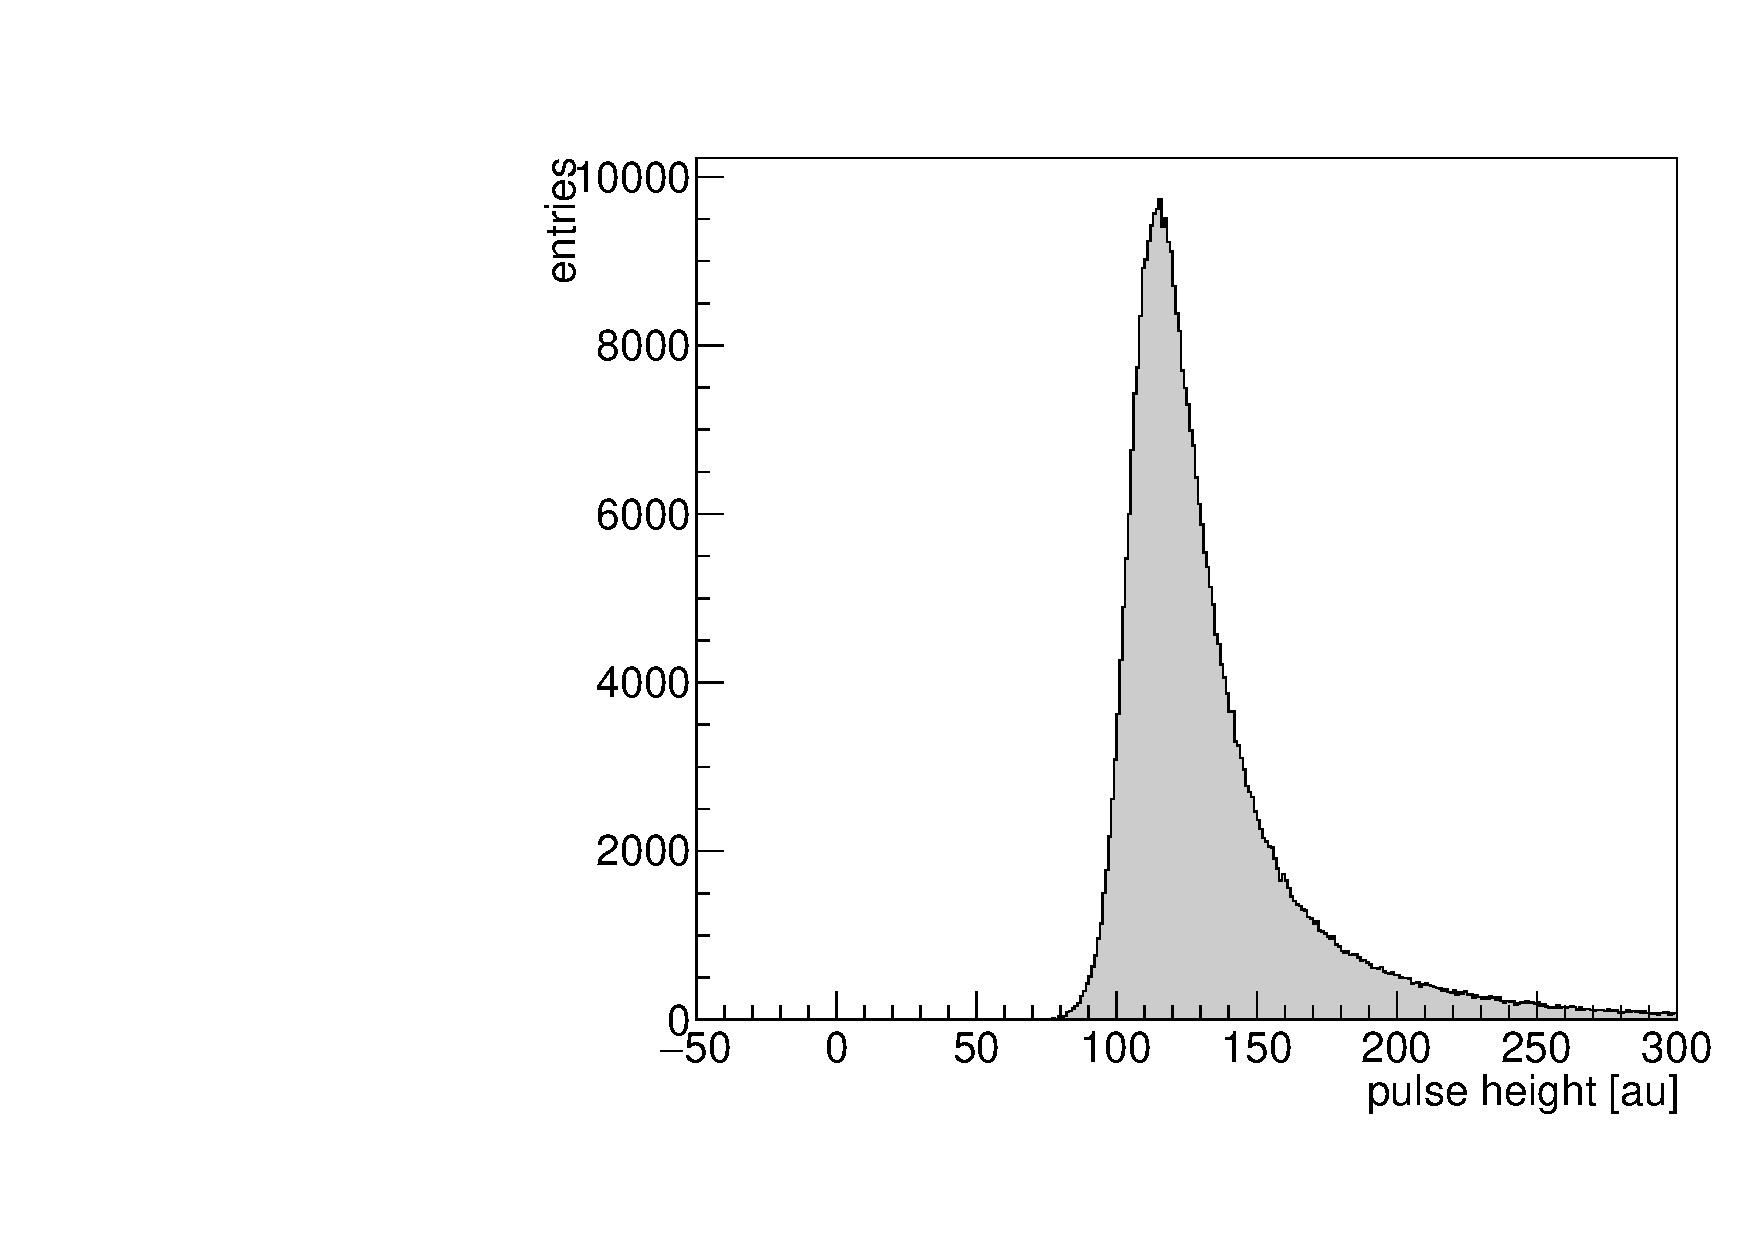
\includegraphics[angle=270, width=\sp]{sDisto}
		\end{subfigure}
		\begin{subfigure}{0.45\textwidth} 
			\centering 
			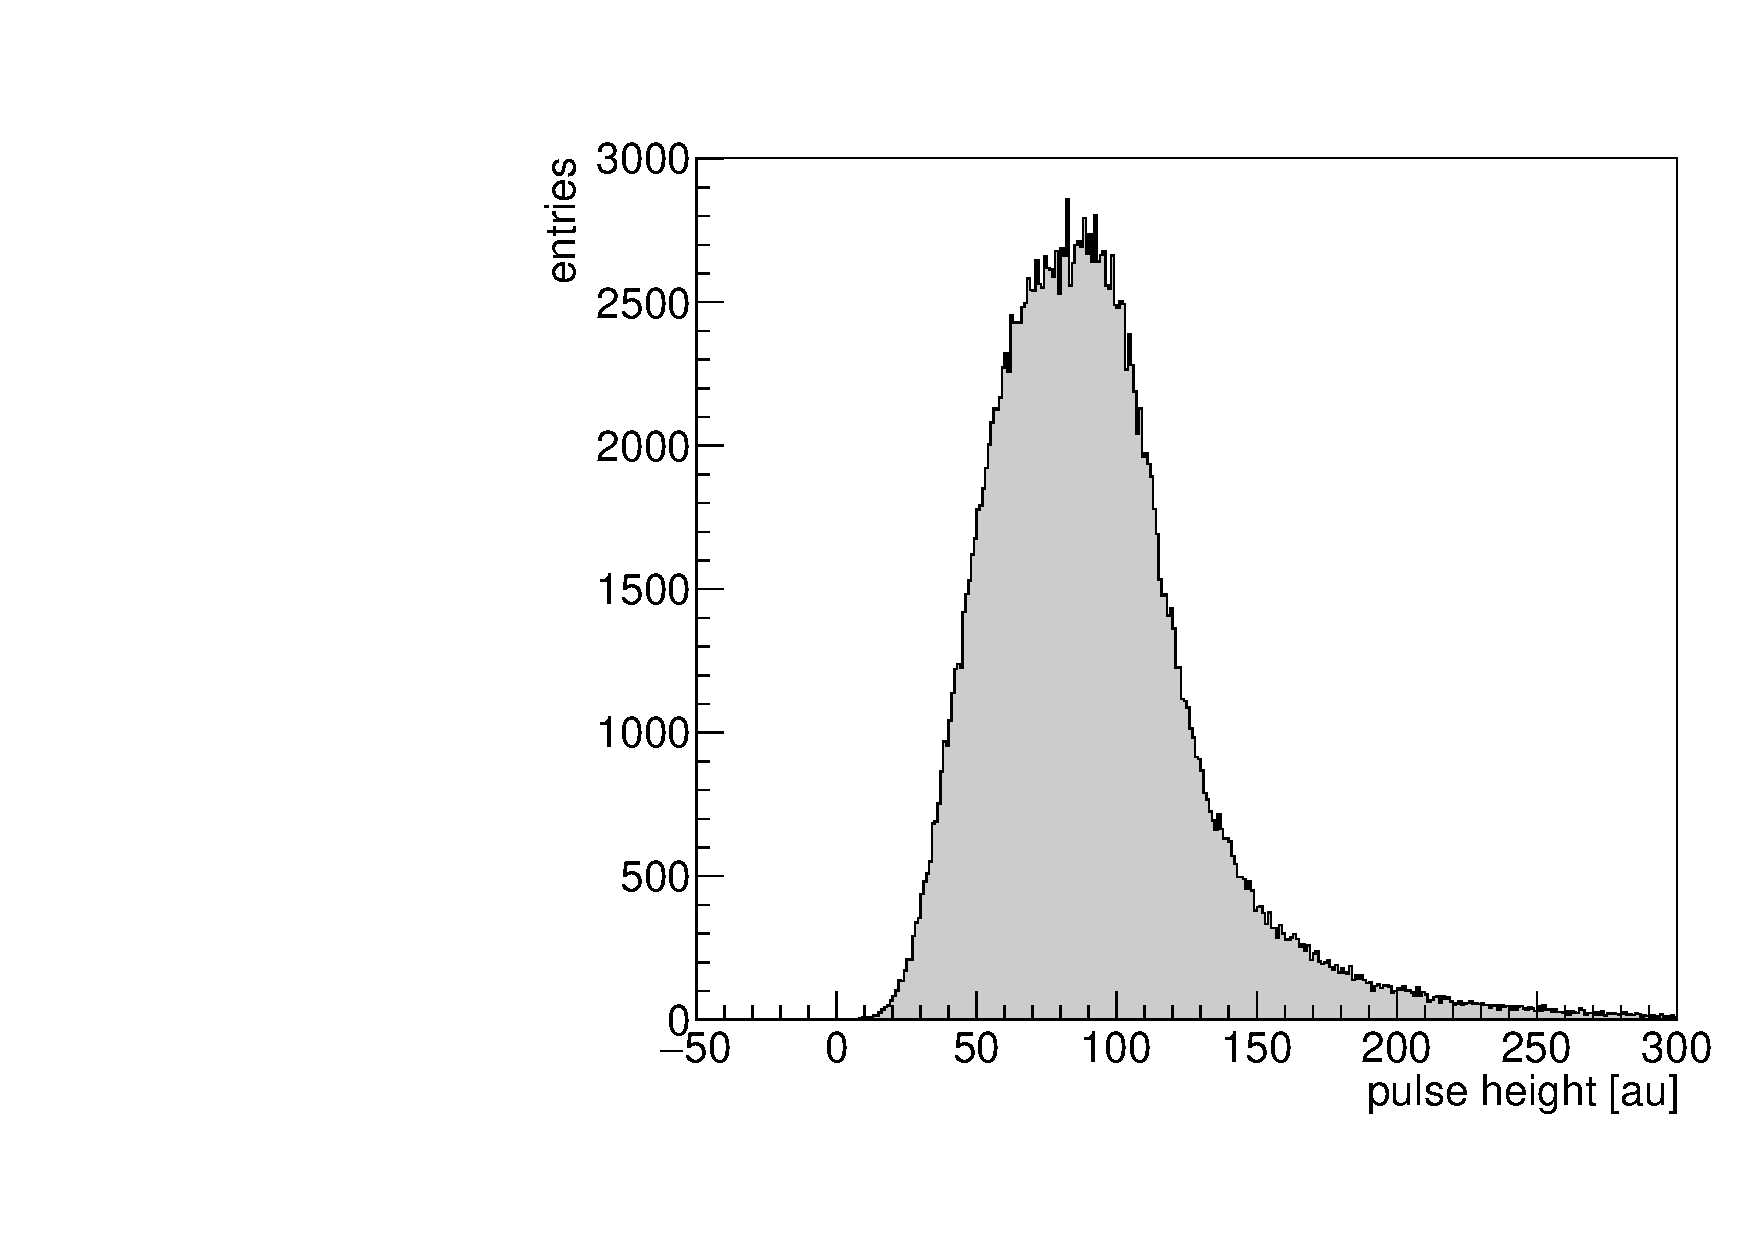
\includegraphics[angle=270, width=\sp]{pDisto}
		\end{subfigure}
	\end{figure}
	\vspace*{-15pt}
	\begin{figure}
	\centering
		\begin{subfigure}{0.45\textwidth} 
			\centering 
			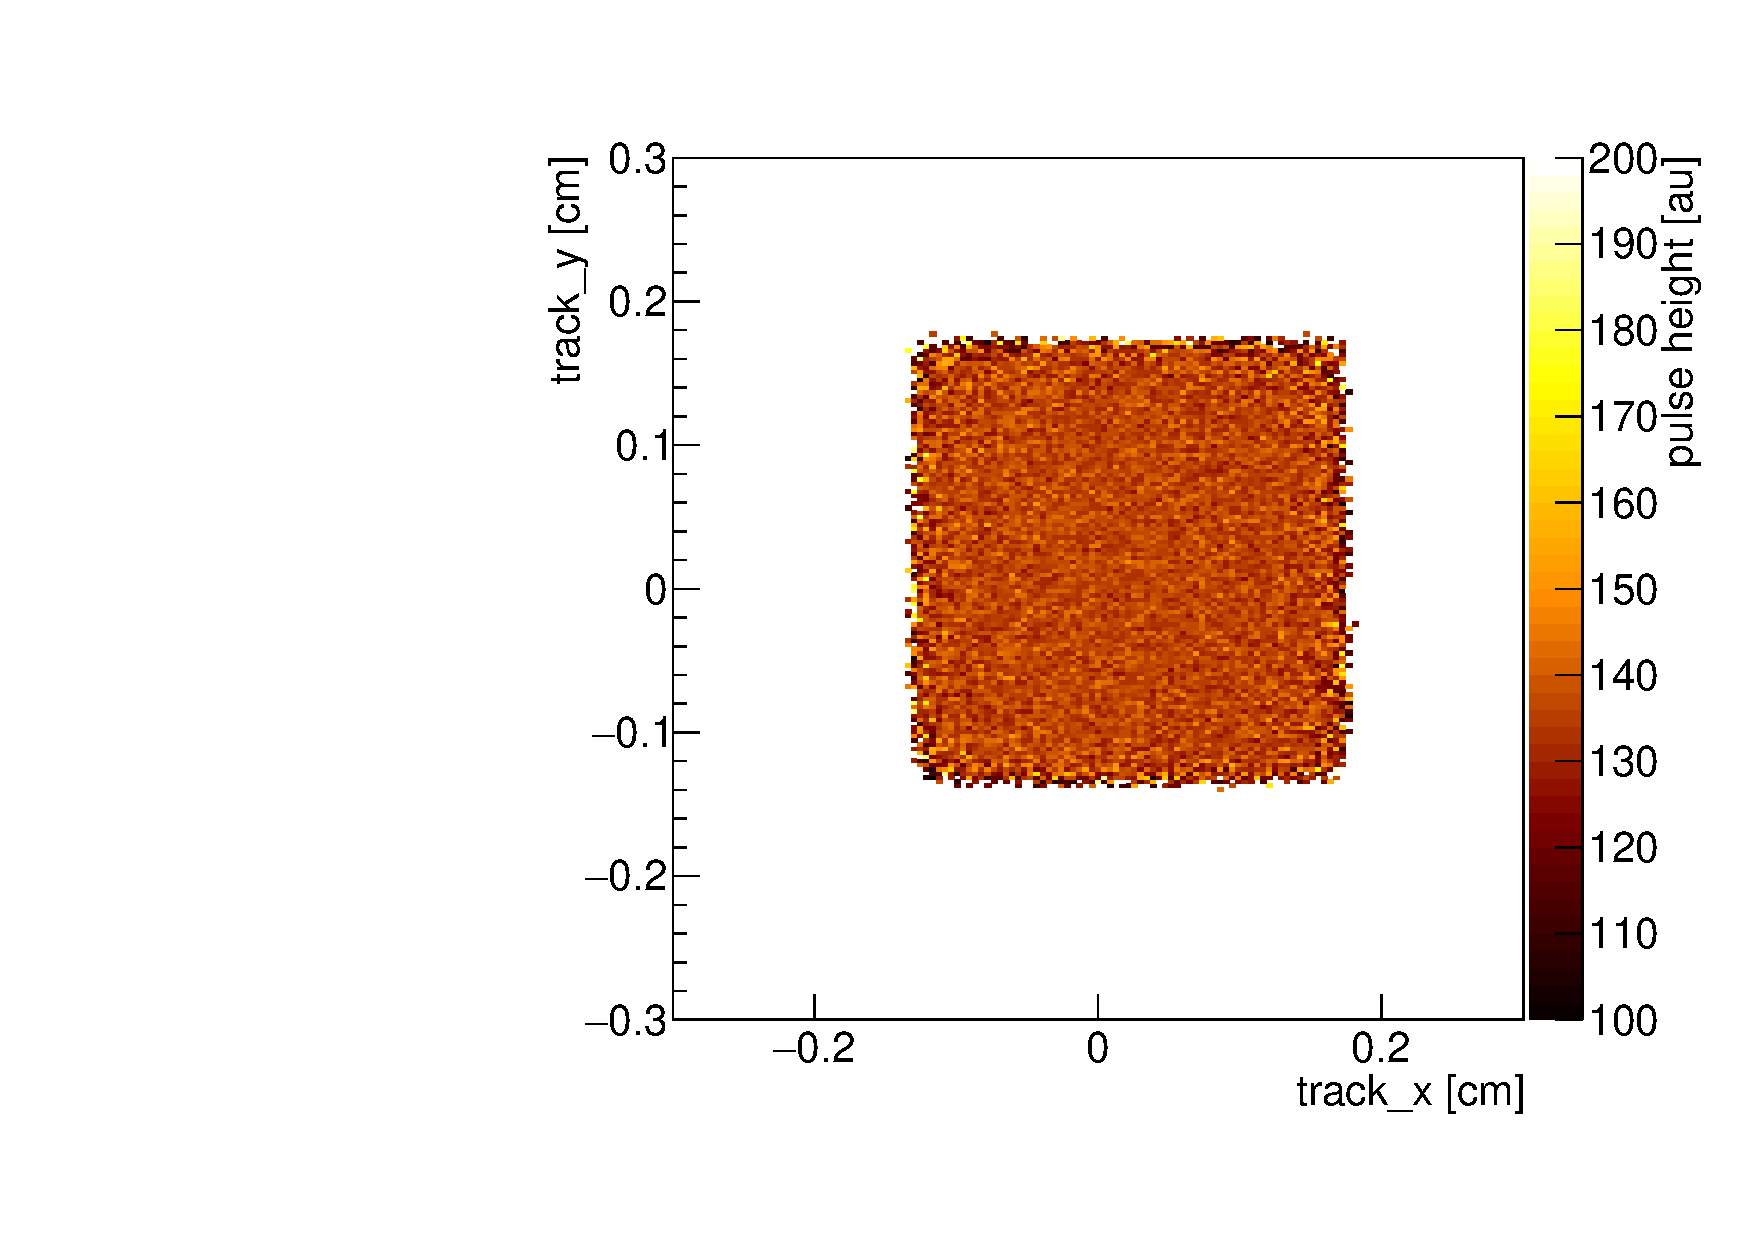
\includegraphics[angle=270, width=\sp]{sSigMap}
			\caption{single-crystalline}
		\end{subfigure}
		\begin{subfigure}{0.45\textwidth} 
			\centering 
			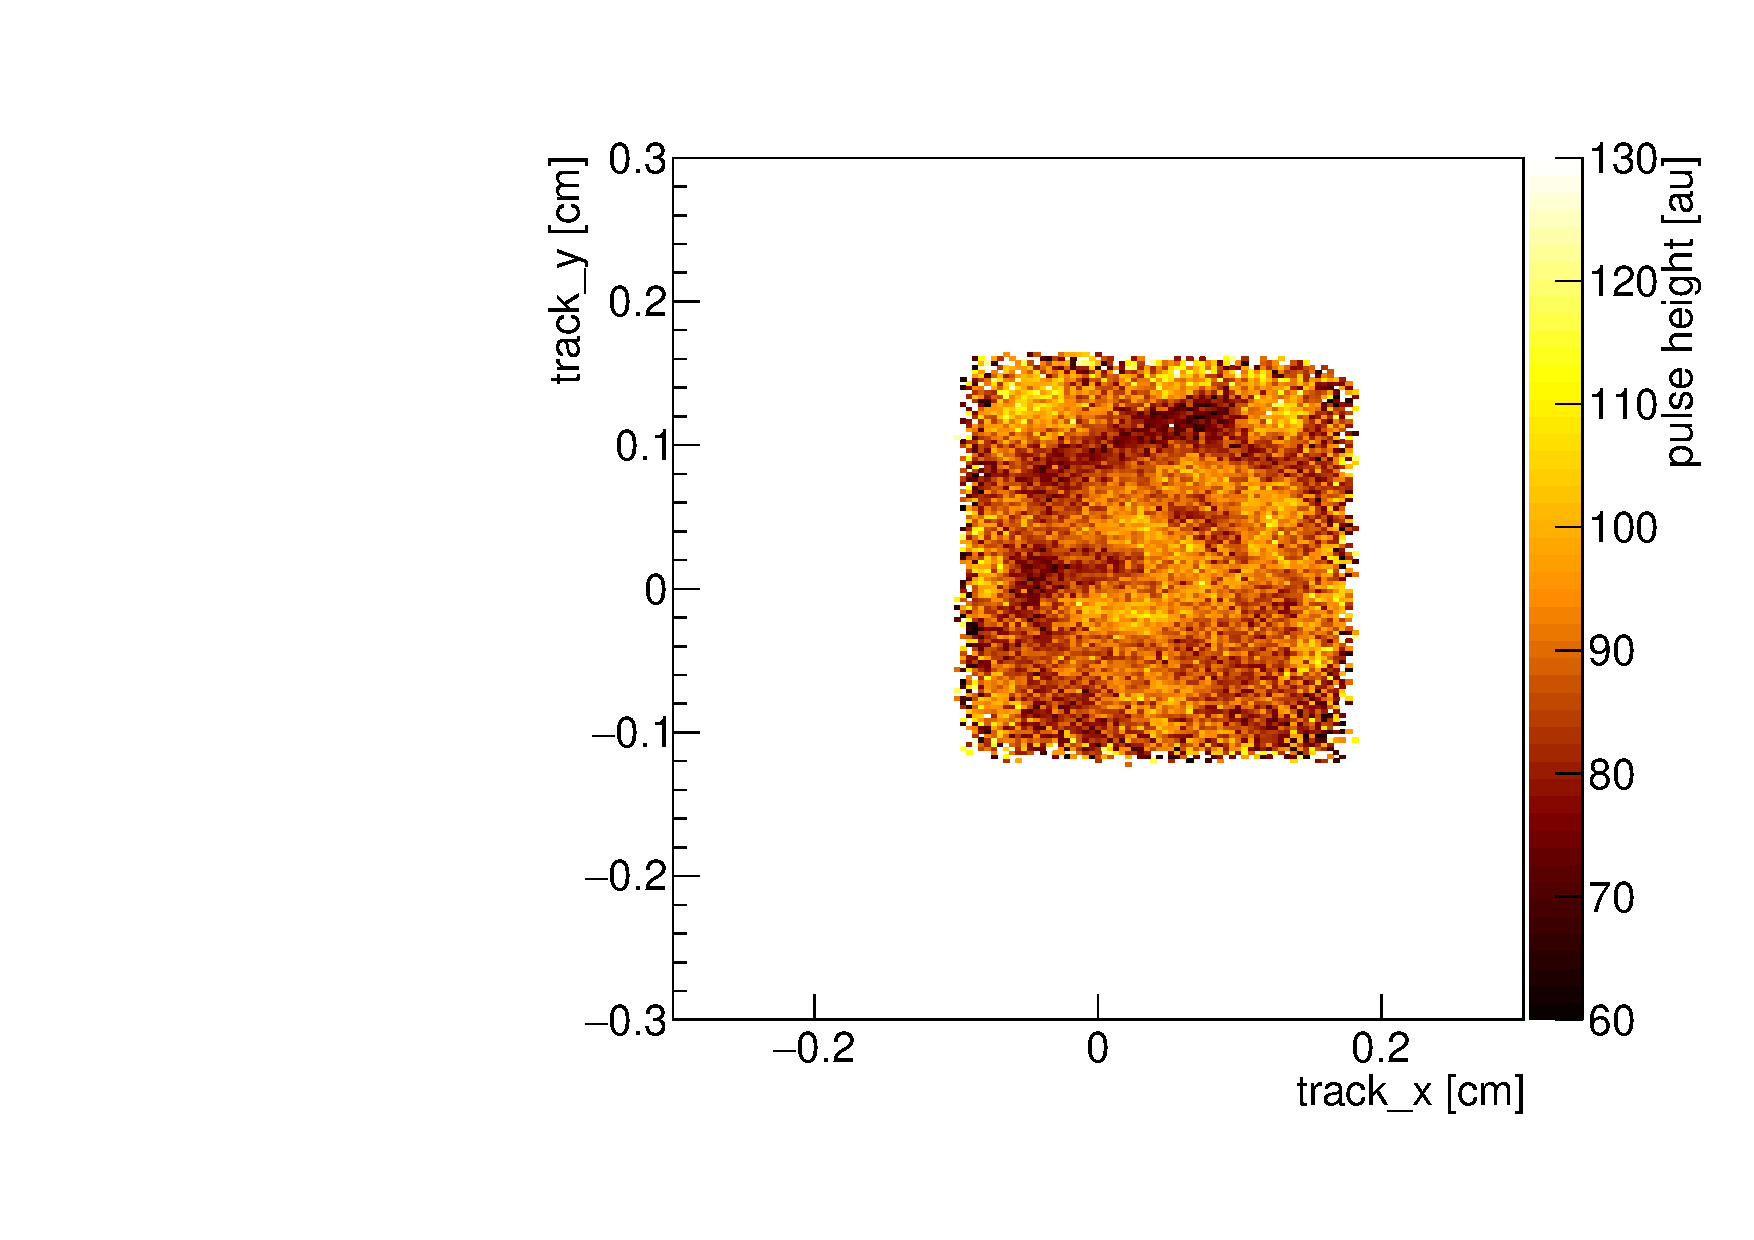
\includegraphics[angle=270, width=\sp]{pSigMap}
			\caption{poly-crystalline}
		\end{subfigure} 
	\end{figure}
\end{frame}
% ============================ new frame ==========================================>
\begin{frame}
	\centering
	\begin{minipage}{3.1cm}
		\centering
		August 2016 - \\unirradiated
		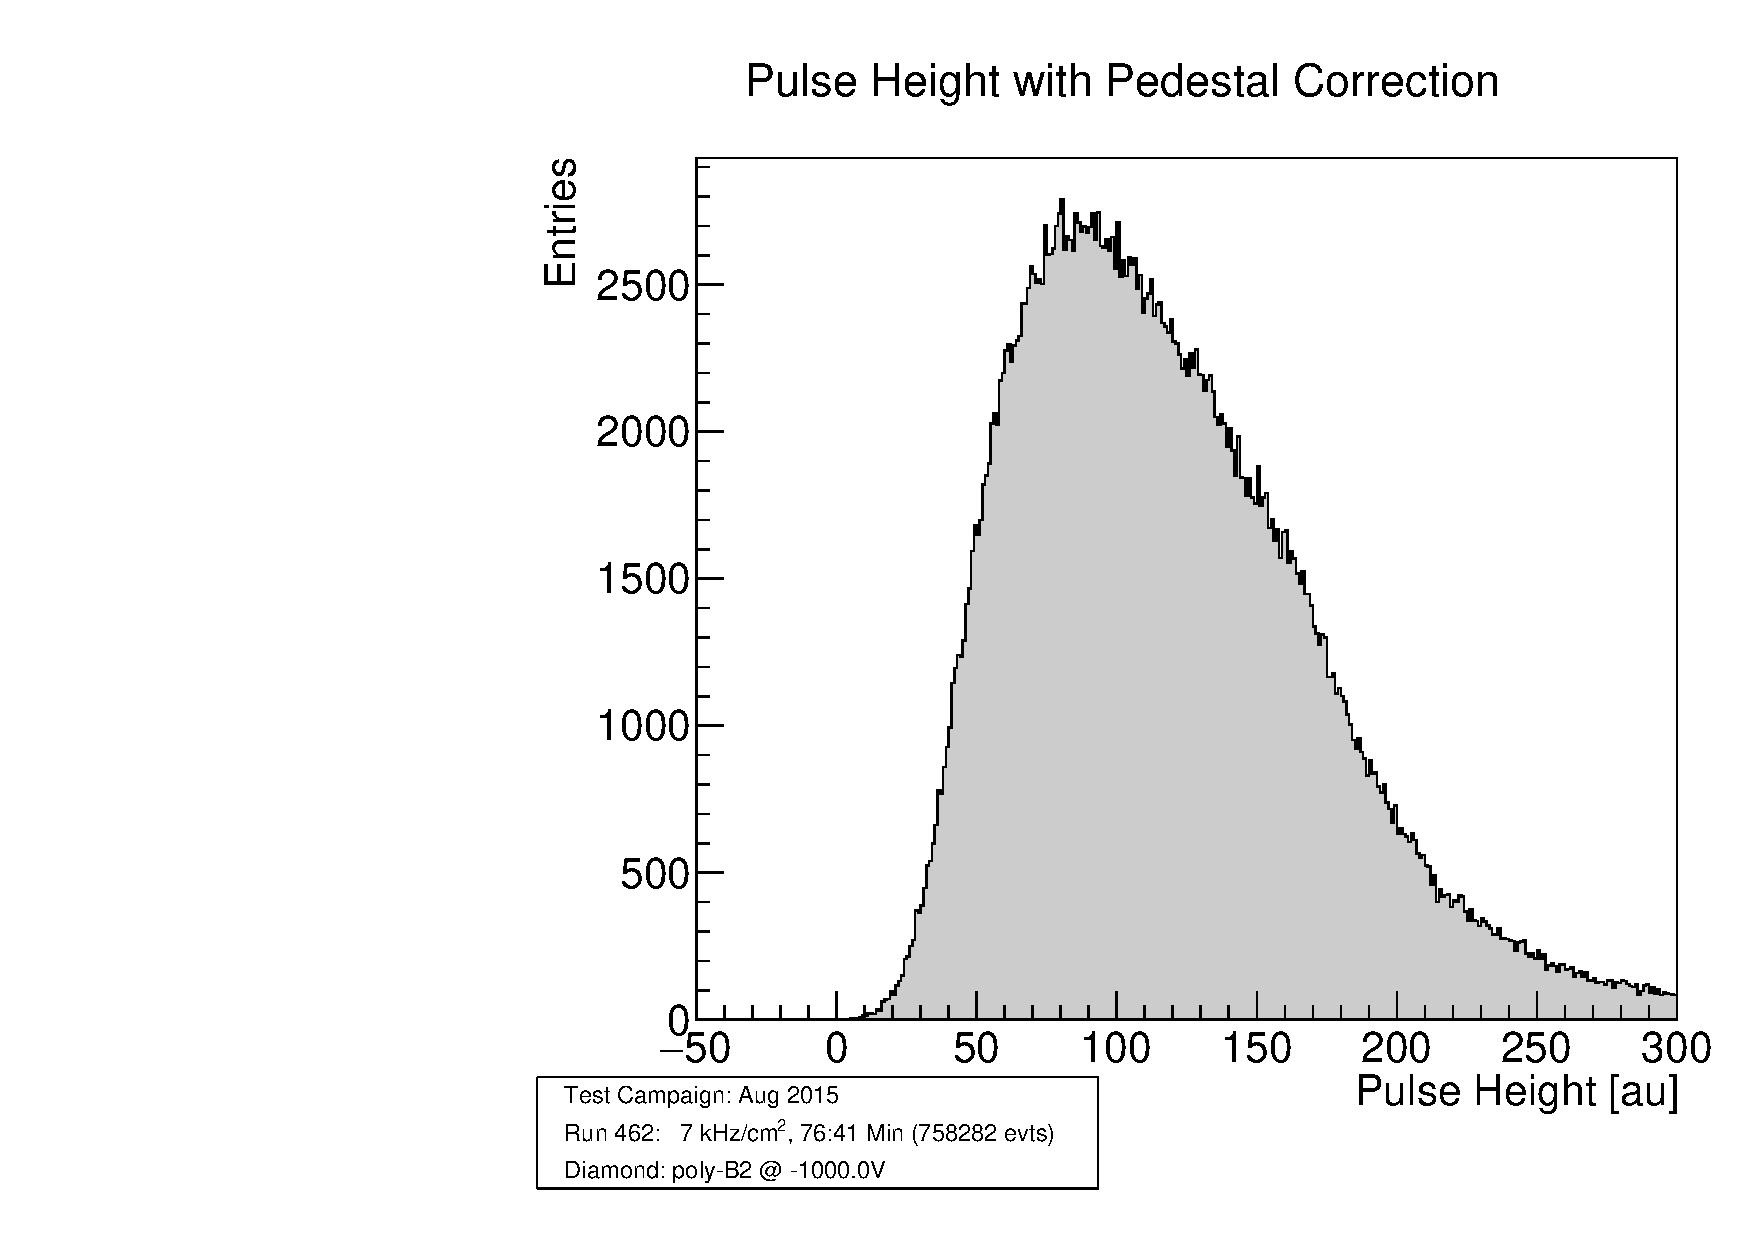
\includegraphics[angle=270, width=3.1cm]{SD462}\\
		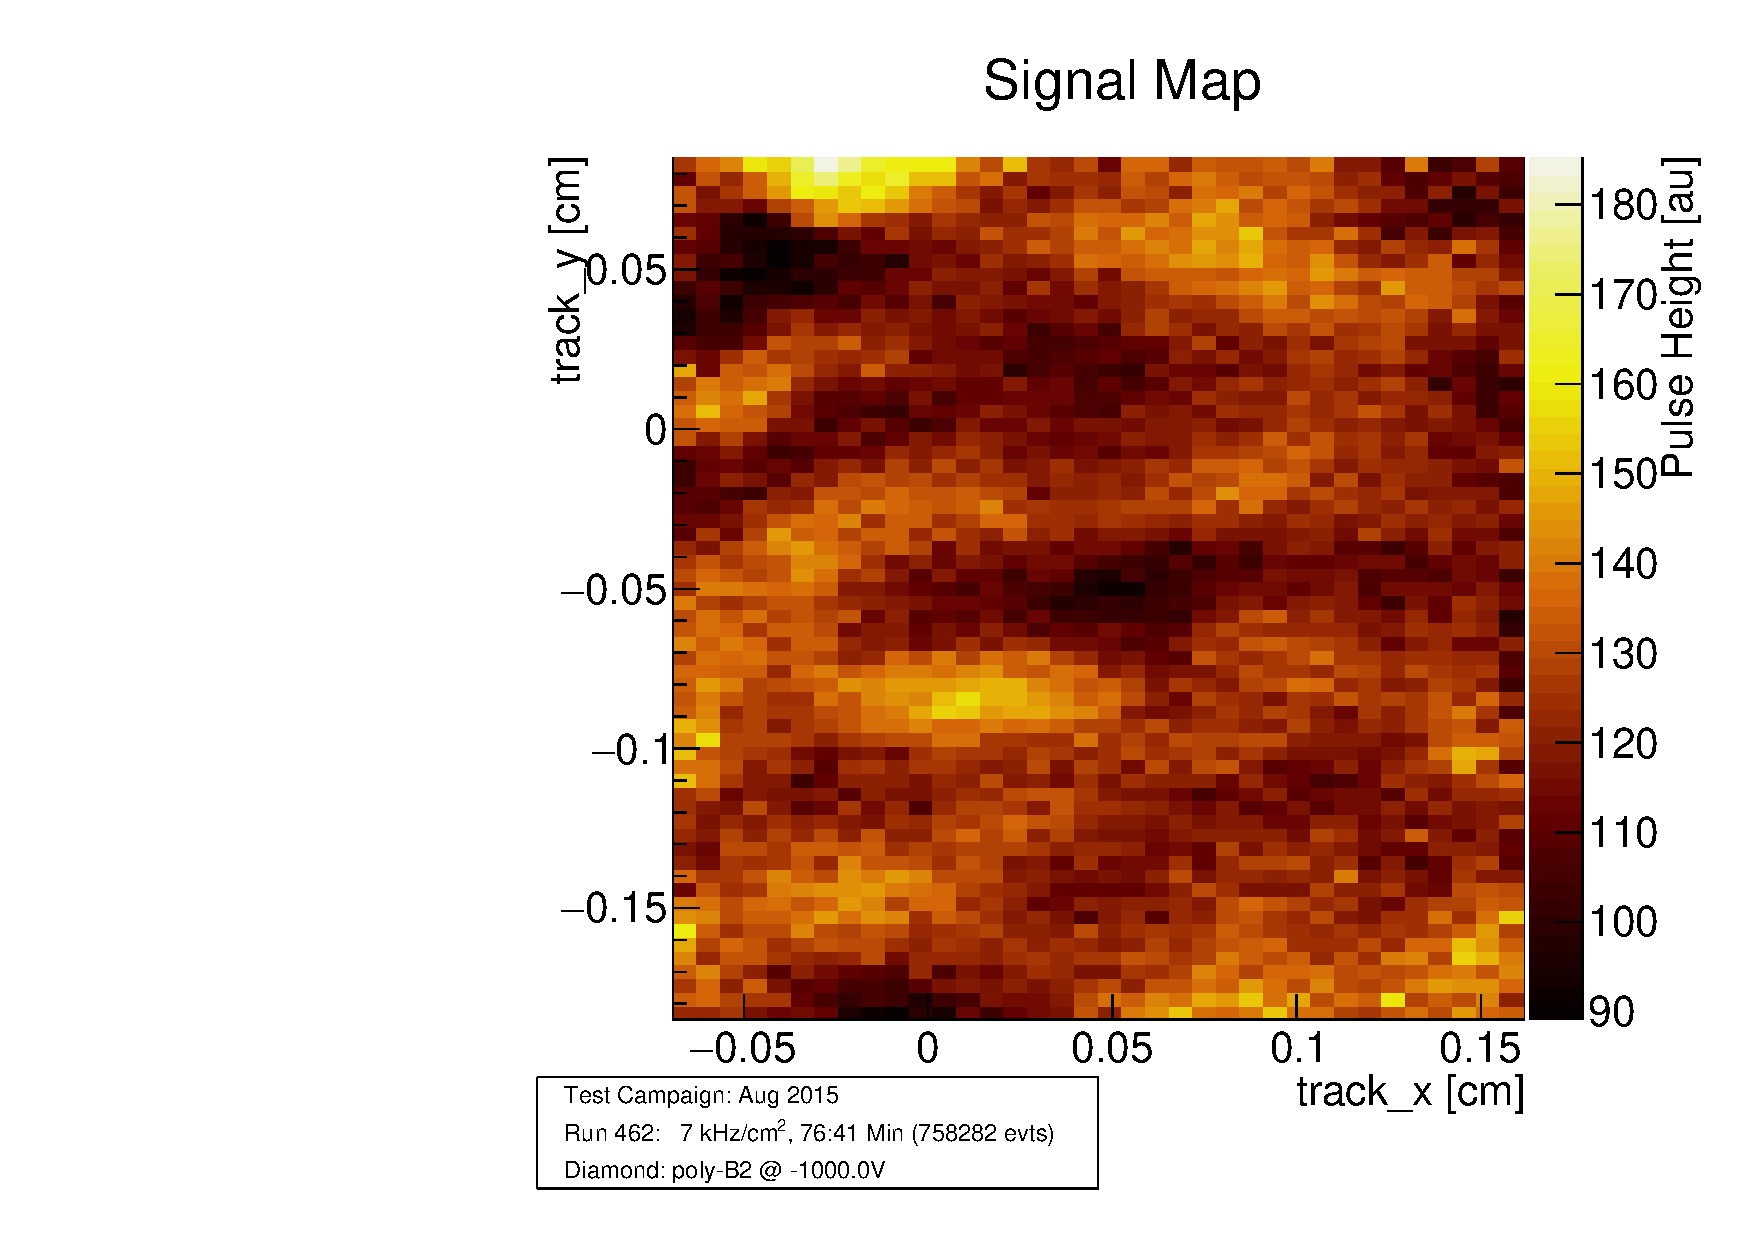
\includegraphics[angle=270, width=3.1cm]{SM462}
	\end{minipage}
	\hspace*{2pt}
	\begin{minipage}{3.1cm}
		\centering
		October 2015 - \SI[exponent-product = \cdot]{5e14}{n/cm^{2}}
		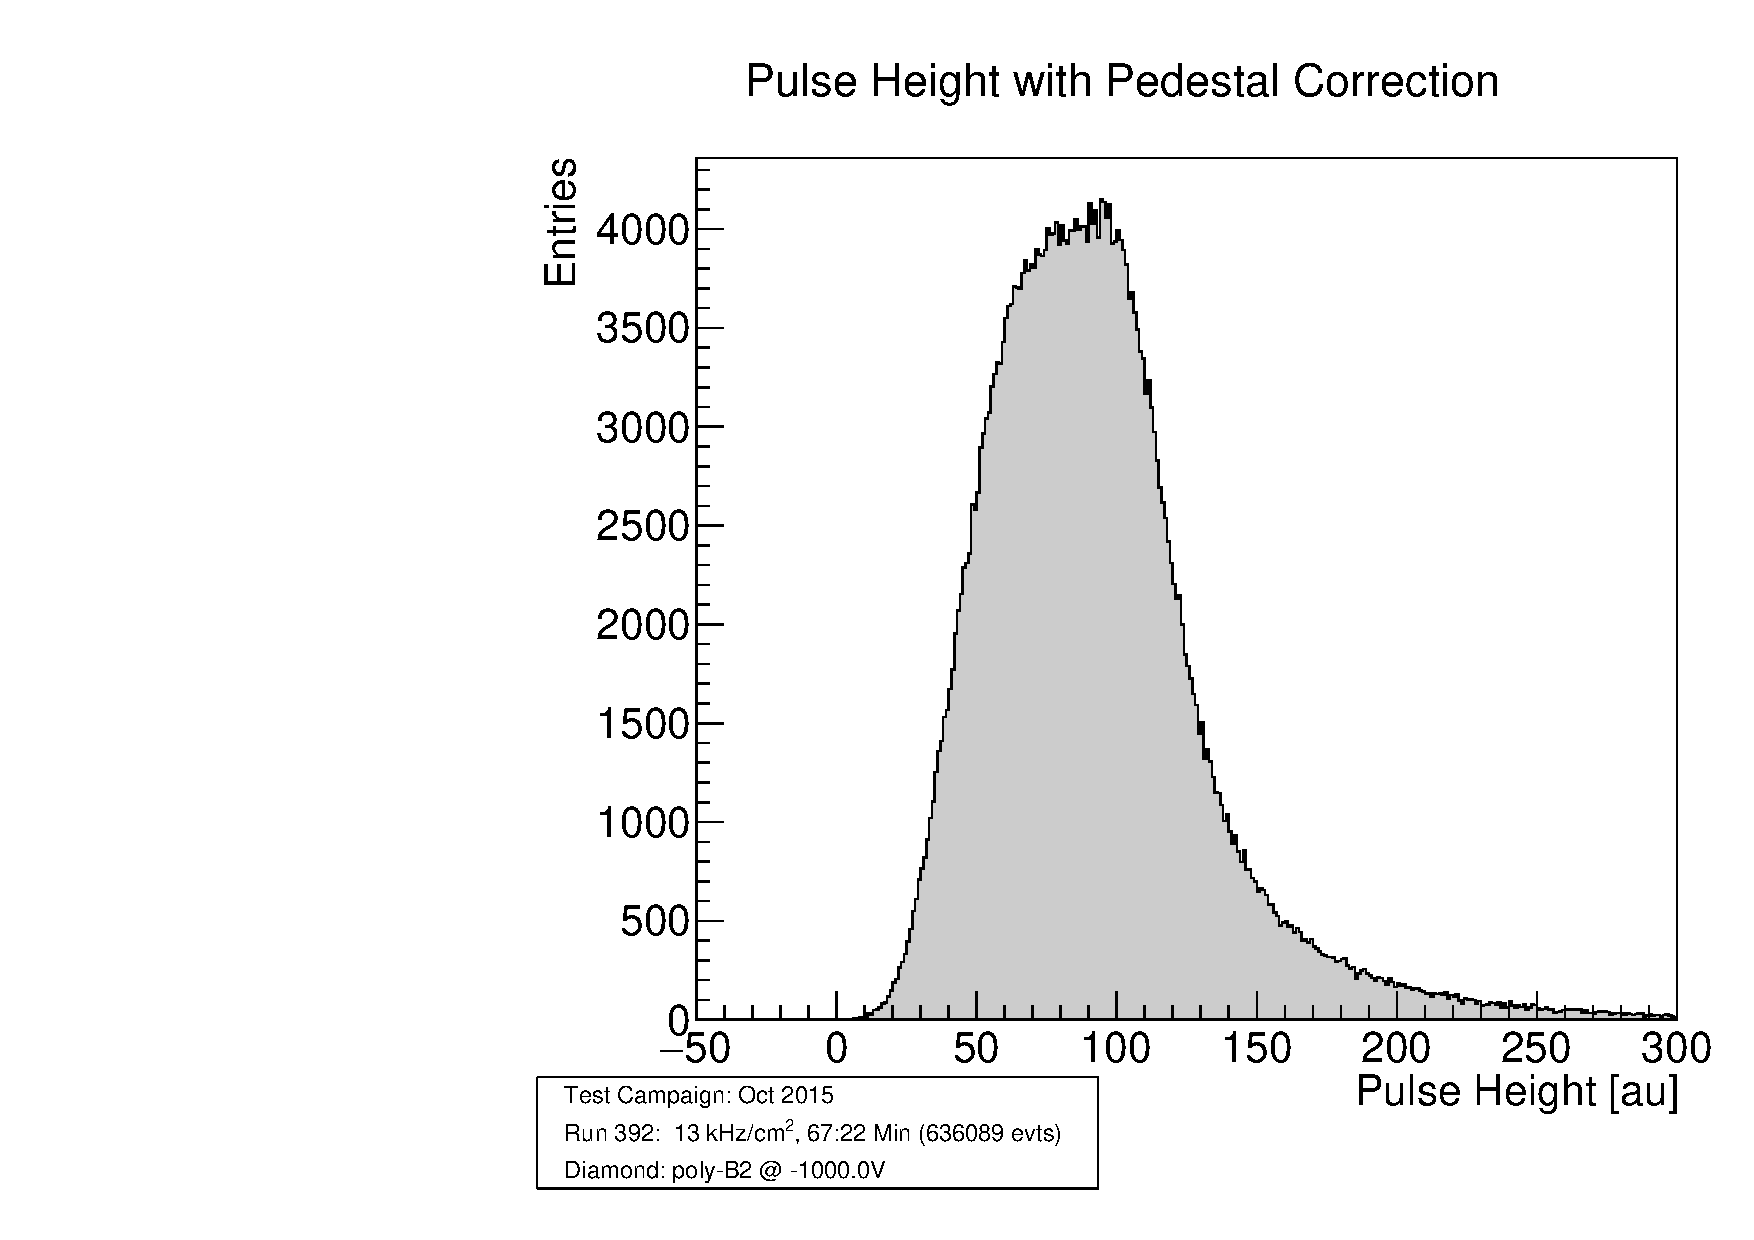
\includegraphics[angle=270, width=3.1cm]{SD392}\\
		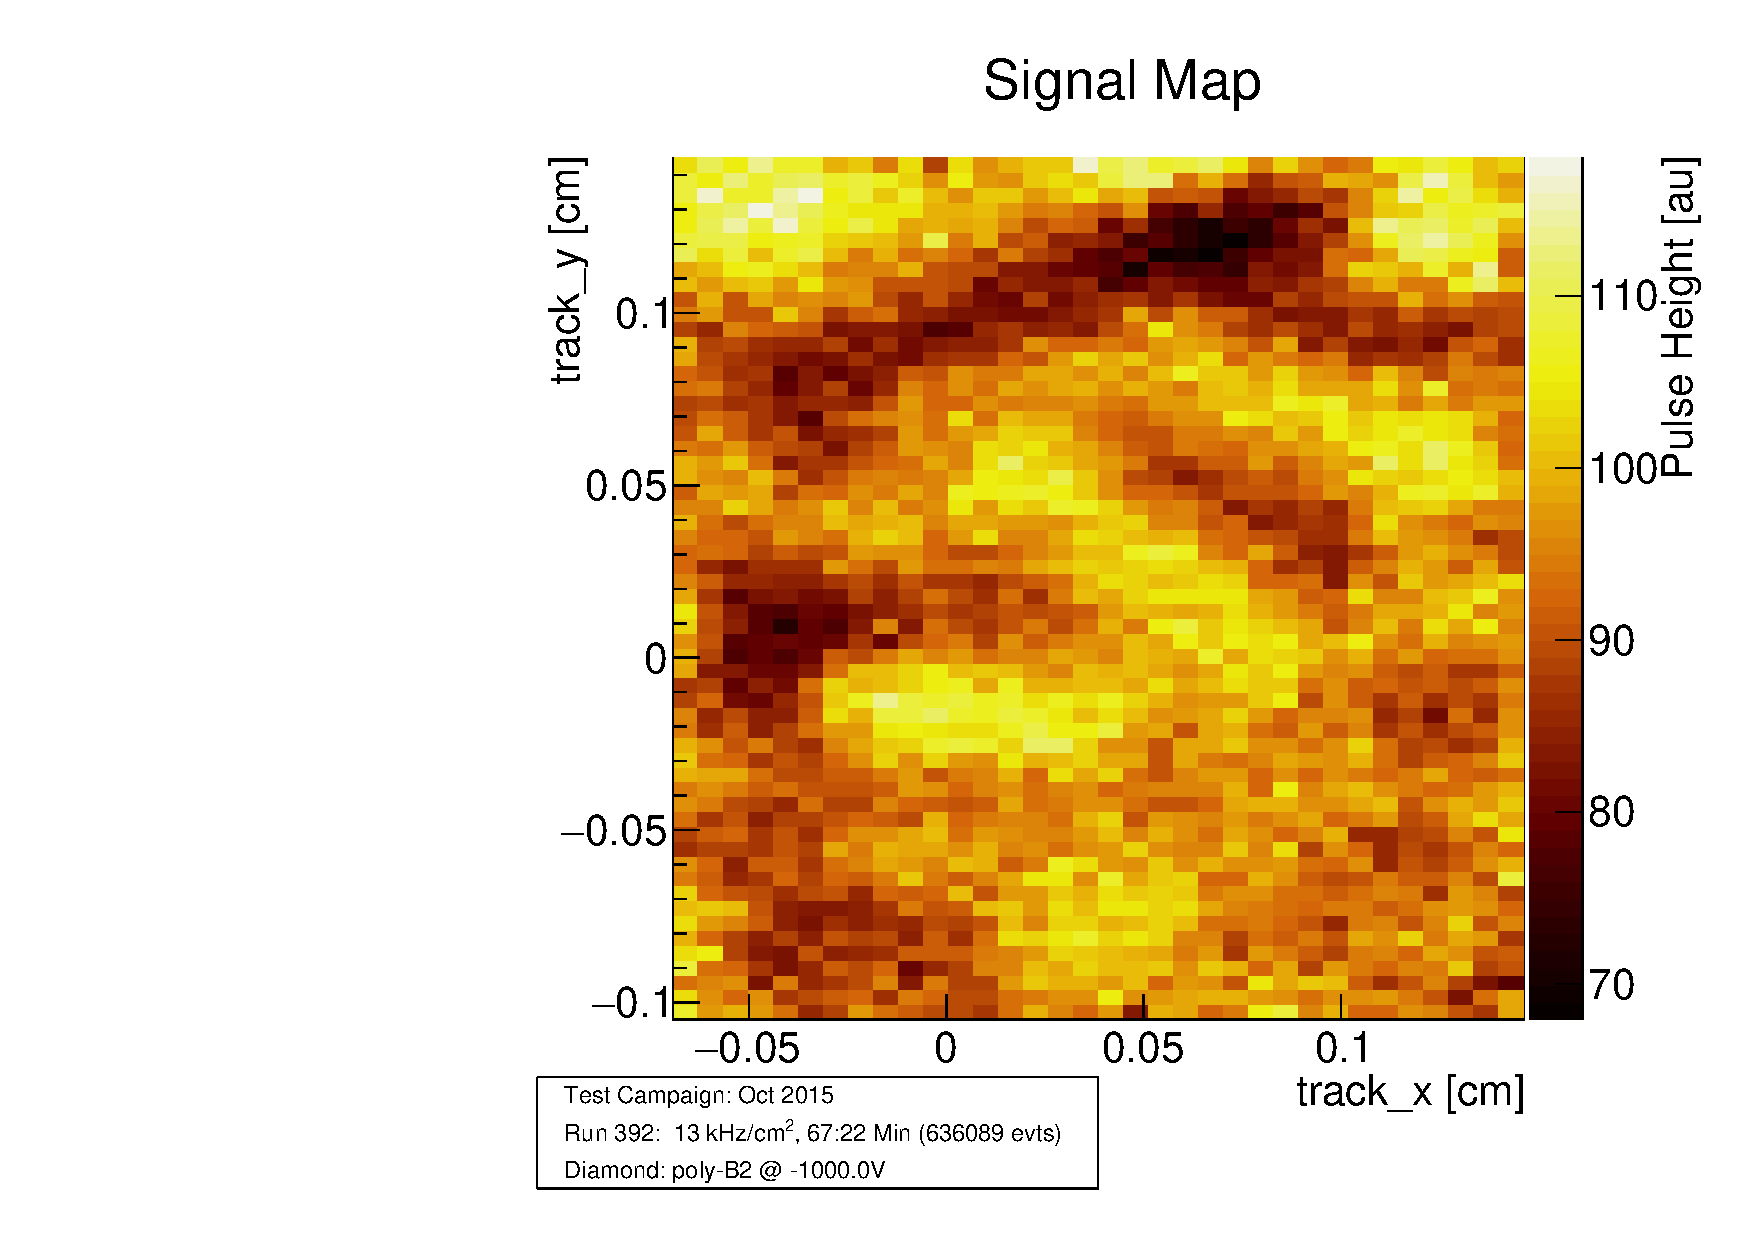
\includegraphics[angle=270, width=3.1cm]{SM392}
	\end{minipage}
	\hspace*{2pt}
	\begin{minipage}{3.1cm}
		\centering
		August 2016 - \SI[exponent-product = \cdot]{1e15}{n/cm^{2}}
		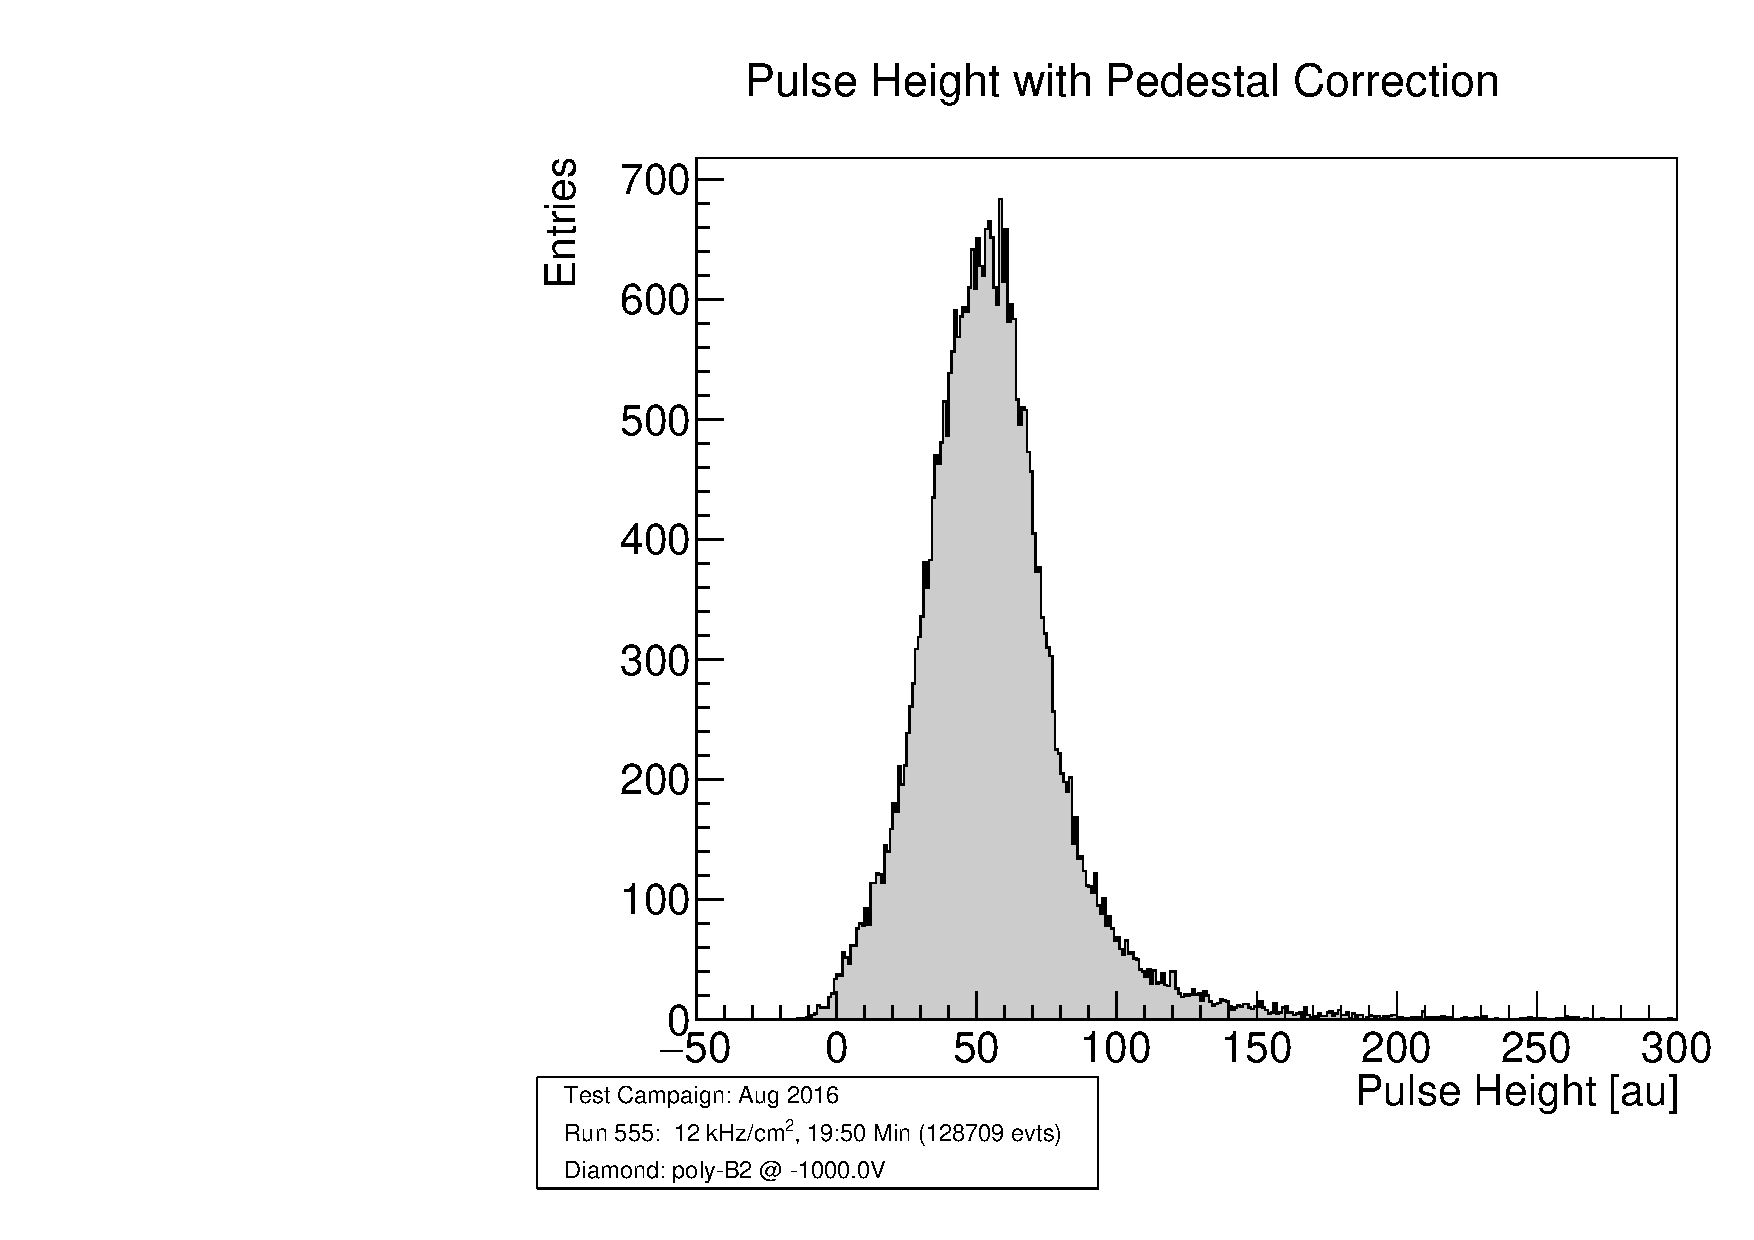
\includegraphics[angle=270, width=3.1cm]{SD555}\\
		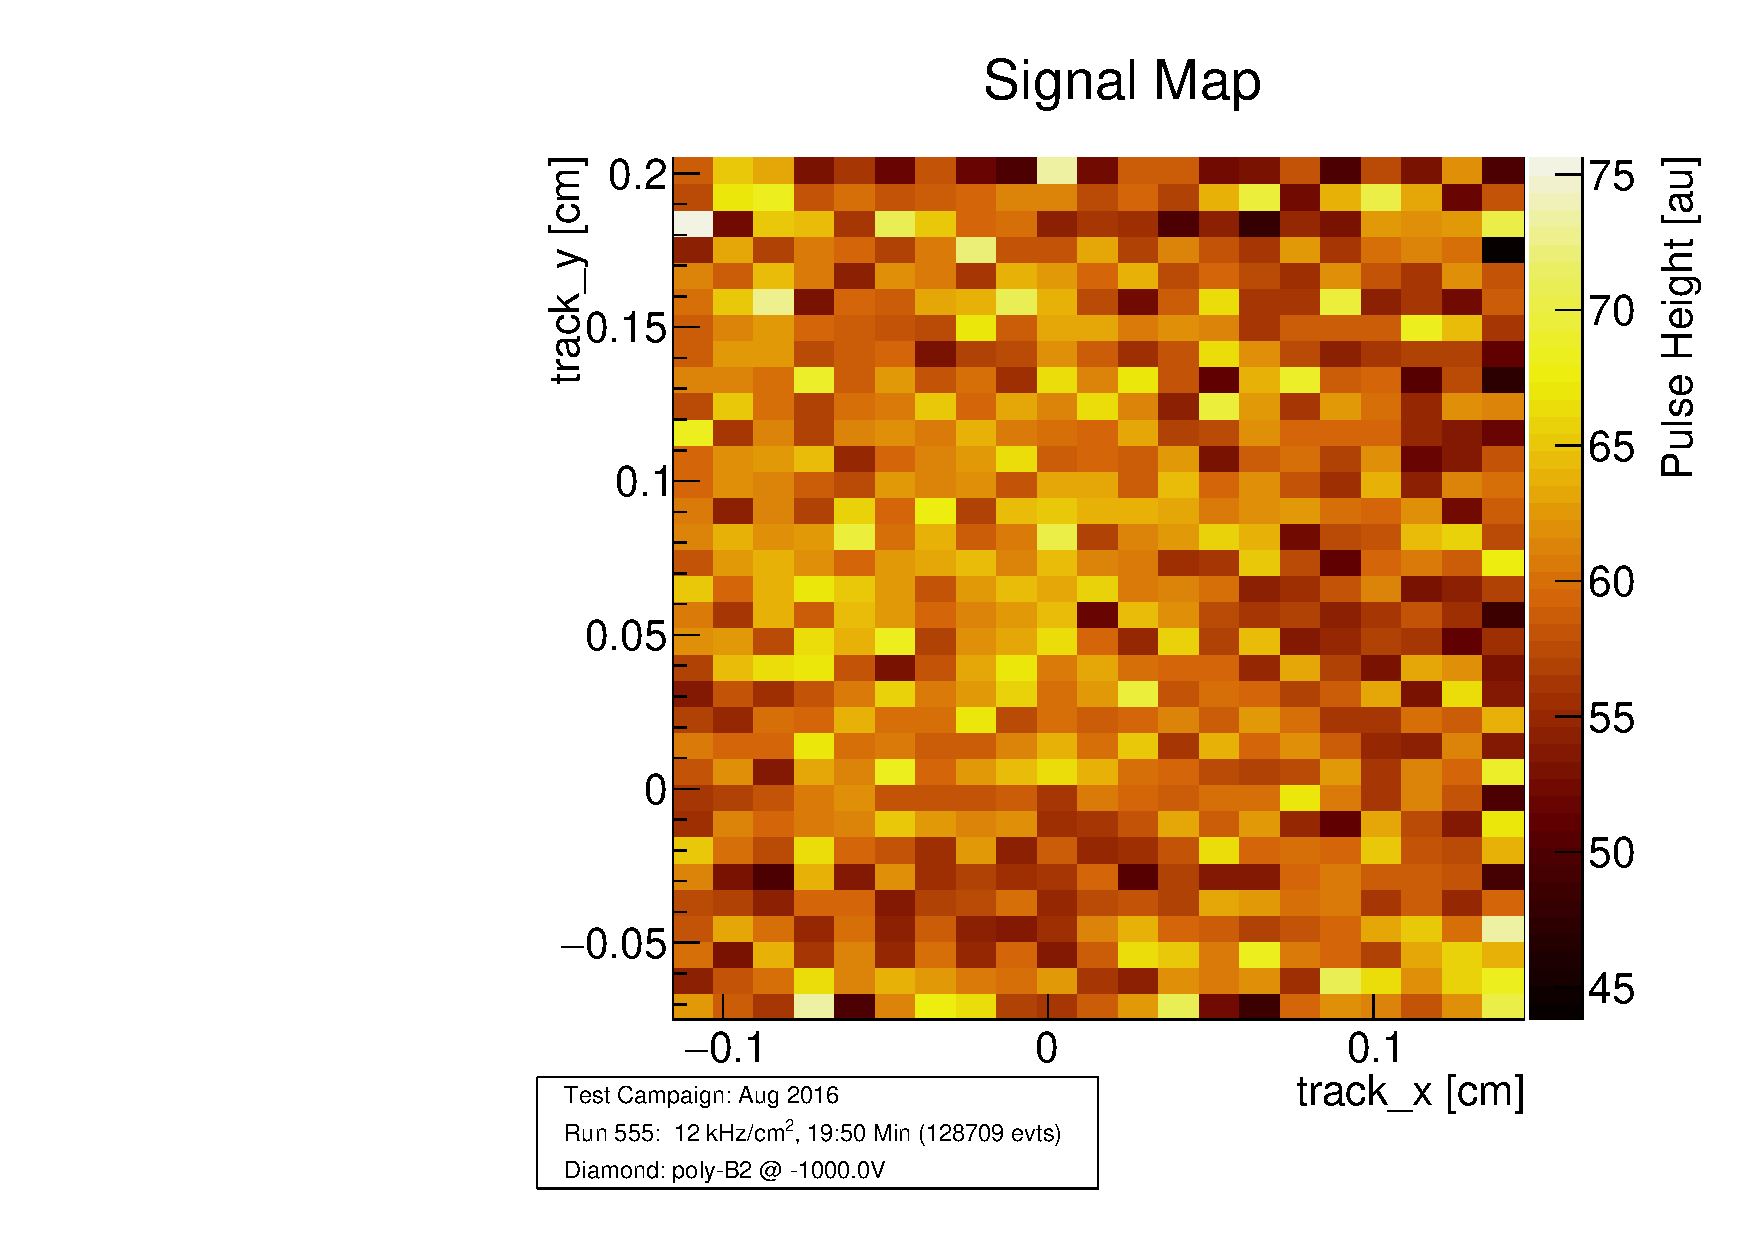
\includegraphics[angle=270, width=3.1cm]{SM555}
	\end{minipage}\s
\end{frame}
% ============================ new frame ==========================================>
% END
